\documentclass[11pt]{article}
\usepackage{graphics,graphicx}
%\usepackage[dvips]{graphics,graphicx}
\DeclareGraphicsExtensions{.ps,.jpg,.eps,.pdf,.png}
\usepackage{boxedminipage,amsmath,amsfonts}
\usepackage{url}
%\usepackage{secdot}
%\usepackage{natbib}
\usepackage{verbatim, moreverb}
\bibliographystyle{plain}



%%%%%
% some other macros
\newcommand{\figurepath}{./figures}
\newcommand{\bibpath}{/Users/kmartin/Documents/files/misc}
\newcommand{\figfiletype}{pdf}

%Brad Bell Macors

% Latex macros defined for all the CppAD documentation:
\newcommand{\T}{ {\rm T} }
\newcommand{\R}{ {\bf R} }
\newcommand{\C}{ {\bf C} }
\newcommand{\D}[2]{ \frac{\partial #1}{\partial #2} }
\newcommand{\DD}[3]{ \frac{\partial^2 #1}{\partial #2 \partial #3} }
\newcommand{\Dpow}[2]{ \frac{\partial^{#1}}{\partial  {#2}^{#1}} }
\newcommand{\dpow}[2]{ \frac{ {\rm d}^{#1}}{{\rm d}\, {#2}^{#1}} }

% Define the hangref environment used for the References list:
\newenvironment{hangref}
  {\begin{list}{}{\setlength{\itemsep}{4pt}
  \setlength{\parsep}{0pt}\setlength{\leftmargin}{+\parindent}
  \setlength{\itemindent}{-\parindent}}}{\end{list}}

% Set the page margins to 1 inch all around:
\marginparwidth 0pt\marginparsep 0pt \topskip 0pt\headsep
0pt\headheight 0pt \oddsidemargin 0pt\evensidemargin 0pt
\textwidth 6.5in \topmargin 0pt\textheight 9.0in
\newtheorem{theorem}{Theorem}


%%%%Added by Leo%%%%
\newcounter{Fig}
\renewcommand{\theFig}{\arabic{Fig}}
\newcommand{\Fig}[2]{\refstepcounter{Fig} \label{#1}
                     {\small\bf Figure \theFig.} {\small\sl #2 \par}}

\setcounter{topnumber}{3}
\renewcommand{\topfraction}{.9}
\setcounter{bottomnumber}{3}
\renewcommand{\bottomfraction}{.9}
\setcounter{totalnumber}{4}
\renewcommand{\textfraction}{.1}
\setlength{\floatsep}{.25in}
\setlength{\intextsep}{.25in}

\setlength{\fboxrule}{2\fboxrule} \setlength{\fboxsep}{3\fboxsep}

\newcommand{\Sa}{8pt}
\newcommand{\Sb}{0pt}

\renewcommand{\_}{{\char"5F}}
\renewcommand{\{}{{\char"7B}}
\renewcommand{\}}{{\char"7D}}
\renewcommand{\^}{{\char"0D}}

\let\accute= \'
\renewcommand{\'}{{\char"0D}}

\newcommand{\bfit}{\bfseries\itshape}

\newlength{\extopskip} \newlength{\exbottomskip}
\setlength{\exbottomskip}{1\baselineskip}
\addtolength{\exbottomskip}{-5.0pt}
\setlength{\extopskip}{1\exbottomskip}
\addtolength{\extopskip}{-1\parskip}

\newenvironment{Example}{\vspace{1\extopskip}\noindent\hspace*{2em}
                         \frenchspacing\small
                         \tt\begin{tabular}{@{}l@{}}}{
                         \end{tabular}\\[1\exbottomskip]}

\newcommand{\Titem}{\item[$\triangleright$]}
\newcommand{\Ditem}{\item[$\diamond$]}

\newenvironment{Itemize}{\begin{quote}\normalsize
   \baselineskip 20pt plus .3pt minus .1pt \begin{itemize}}
   {\end{itemize}\end{quote}}
   % Set path to folder containing figures
\newcommand{\FigureFolder}{figures}

\begin{document}

\title{Optimization Services 1.0 User's Manual }
\vskip 2in
\author{Robert Fourer, Jun Ma, Kipp Martin, Wayne Sheng}
\maketitle

\begin{abstract}
This is the User's Manual for the Optimization Services (OS) project.  The objective of  (OS) is to provide a general framework consisting of a set of standards for representing optimization instances, results, solver options, and communication between clients and solvers in a distributed environment using Web Services. This COIN-OR project provides C++ and Java source code for libraries and executable programs that implement OS standards.   The OS library includes a robust solver and modeling language interface (API) for linear, nonlinear and other types of optimization problems.   Also included is the C++ source code for a  command line executable {\tt OSSolverService}  for reading problem instances (OSiL format, nl format, MPS format) and calling a solver either locally or on a remote server.  Finally,  both Java source code and a Java war, are provided for users who wish to set up a solver service on a server running Apache Tomcat.   See the Optimization Services (OS) Home Site \url{www.optimizationservices.org} and the COIN-OR Trac page \url{projects.coin-or.org/OS} for more information.
\end{abstract}


\newpage
\tableofcontents
\listoffigures
\listoftables
\hyphenation{com-plex-Type}



%\noindent\hrulefill
\newpage

\section{The Optimization Services (OS) Project}

The objective of Optimization Services (OS) is to provide a general framework consisting of a set of standards for representing optimization instances, results, solver options, and communication between clients and solvers in a distributed environment using Web Services. This COIN-OR project provides source code for libraries and executable programs that implement OS standards.  See the COIN-OR Trac page \url{projects.coin-or.org/OS} or the Optimization Services (OS) Home Site \url{www.optimizationservices.org}   for more information. The OS project provides the following:

\begin{itemize}
\item[1.]  A set of XML based standards for representing optimization instances (OSiL), optimization results (OSrL), and optimization solver options (OSoL). There are other standards, but these are the main ones. The schemas for these standards are described in Section   \ref{section:schemadescriptions}.


\item[2.]  Open source libraries  that support and implement many of the standards.

\item[3.]  A robust solver and modeling language interface (API) for linear and nonlinear optimization problems.  Corresponding to the OSiL problem instance representation there is an in-memory object,  {\tt OSInstance}, along with a set of  {\tt get()},   {\tt set()}, and {\tt calculate()} methods for accessing and creating problem instances.
This is a very general API for linear, integer, and nonlinear programs. Extensions for other major types of optimization problems are also in the works. Any modeling language that can produce OSiL can easily communicate with any solver that uses the OSInstance API.   The {\tt OSInstance} object is described in more detail in Section \ref{section:osinstanceAPI}. The nonlinear part of the API is based on the COIN-OR project \url{projects.coin-or.org/CppAD} by Brad Bell but is written in a very general manner and could be used with other algorithmic differentiation packages. More detail on algorithmic differentiation is provided in Section \ref{section:ad}.


\item[4.]  A  command line executable {\tt OSSolverService}  for reading problem instances (OSiL format, AMPL  nl format,  MPS format) and calling a solver either locally or on a remote server.  This is described in Section \ref{section:ossolverservice}.


\item[5.] Utilities that convert AMPL nl files into the OSiL XML format and MPS files into the OSiL XML format.  This is described in Section \ref{section:osmodelinterfaces}.


\item[6.]  Standards that facilitate the communication between clients and optimization solvers using Web Services.  In  Section \ref{section:osagent} we describe the {\tt OSAgent} part of the OS library that is used to create Web Services
 SOAP packages with OSiL instances and contact a server for solution.

\item[7.]  An executable program {\tt amplClient} that is designed to work with the AMPL modeling language. The {\tt amplClient} appears as a ``solver'' to AMPL and, based on options given in AMPL, contacts solvers either remotely or locally to solve instances created in AMPL. This is described in Section \ref{section:amplclient}.

\item[8.]  Server software that works with Apache Tomcat and Apache Axis.
This software uses Web Services technology and acts as middleware between the client that creates the instance, and solver on the server that optimizes the instance and returns the result. This is illustrated in Section  \ref{section:tomcat}
\end{itemize}


\section{Quick Roadmap}\label{section:roadmap}

If you want to:

\begin{itemize}
\item Download  the OS source code -- see Section \ref{section:download}.


\item Build the OS project from the source code -- see Section \ref{section:build}.

\item Use the OS library to build model instances or use solver APIs -- see Sections  \ref{section:osmodelinterfaces},  \ref{section:ossolverinterfaces}, and \ref{section:osinstanceAPI}.

\item Use the OSSolverService to read files in nl, OSiL, or MPS format and call a solver locally or remotely -- see Section \ref{section:ossolverservice}.


\item Use AMPL to solve problems either locally or remotely with a COIN-OR solver, Cplex, GLPK, Knitro, or LINDO -- see Section \ref{section:amplclient}.


\item Build a remote solver service using Apache Tomcat -- see Section \ref{section:tomcat}.

\item Use MATLAB to generate problem instances in OSiL format and call a solver either remotely or locally -- see Section \ref{section:usingmatlab}.

\item Use the OS library for algorithmic differentiation (in conjunction with COIN-OR CppAD) -- see Section \ref{section:ad}.
\end{itemize}





\section{Downloading the OS Project}\label{section:download}

The OS project is an open-source project  with source code under the Common Public License (CPL). This project was created by Robert Fourer, Jun Ma, and Kipp Martin. The code has been written primarily by Jun Ma, Kipp Martin, Robert Fourer, and Huanyuan Sheng.  Jun Ma and Kipp Martin are the COIN project leaders for OS.    Below we describe different methods for obtaining the C++ source code or the binaries.




\subsection{Obtaining OS Source Code Using Subversion (SVN)}\label{section:svn}

The C++ source code can be obtained using the Subversion version control package.  Users with Unix operating systems will most likely have a command line svn client.  If an svn client is not present, see \url{http://subversion.tigris.org} to download an svn client.   For Windows users we recommend the  SVN client  TortoiseSVN.  See \url{tortoisesvn.tigris.org}.  The TortoiseSVN client is integrated within the Windows  Explorer.

For Users on a Unix system such as Linux, Solaris, Mac OS X, etc., the source code is obtained as follows. In a command window execute:

\begin{verbatim}
svn co https://projects.coin-or.org/svn/OS/releases/1.0.0 COIN-OS
\end{verbatim}


It is possible that on some systems you may get a message such as:
\begin{verbatim}
Error validating server certificate for 'https://projects.coin-or.org:443':
 - The certificate is not issued by a trusted authority. Use the
   fingerprint to validate the certificate manually!
Certificate information:
 - Hostname: projects.coin-or.org
 - Valid: from Jun 10 22:51:18 2007 GMT until Jun 15 21:00:28 2009 GMT
 - Issuer: 07969287, http://certificates.godaddy.com/repository, GoDaddy.com, In
c., Scottsdale, Arizona, US
 - Fingerprint: f7:26:0f:bb:e1:94:a5:23:7f:5c:cb:c3:9a:c4:74:51:e5:c7:4d:29
(R)eject, accept (t)emporarily or accept (p)ermanently?
\end{verbatim}

If so, select {\tt (p)} and you should not get this message again.

On Windows with TortoiseSVN, create a directory {\tt COIN-OS} in the desired location and right-click on this directory.   Select the menu item {\tt SVN Checkout ...} and in the textbox, {\tt URL of Repository}
give the URL for the version of the OS project you wish to checkout, e.g. https://projects.coin-or.org/svn/OS/stable/1.0.


Now build the project as described in  Section \ref{section:build}.

For the rest of this documentation, we assume that  {\tt COIN-OS} is the name of the root directory of the OS project and that the user has defined an environment variable {\tt OS} that is the path to {\tt COIN-OS}.  The {\tt COIN-OS} directory structure is illustrated in Figure \ref{figure:osprojectrootdir}. OS source code is mainly contained inside of the OS subdirectory. Other first level subdirectories are mostly external projects (COIN-OR or third party) that the OS project depend on.


\begin{figure}
\centering
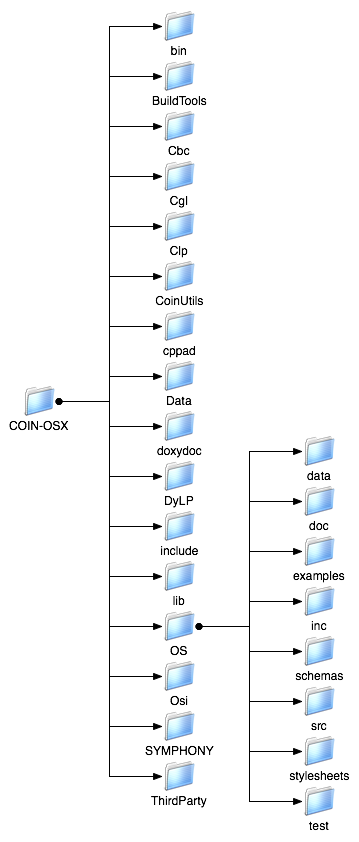
\includegraphics[scale=0.7]{\figurepath/OSProjectRootDirectory.png}
\caption{The OS project root directory.}
\label{figure:osprojectrootdir}
\end{figure}

For more information on downloading the OS project or other COIN-OR projects using SVN see \url{https://projects.coin-or.org/BuildTools/wiki/user-download#DownloadingtheSourceCode}.

The Java source code for the setting up a solver service with Apache Tomcat is checked out as follows:
\begin{verbatim}
svn co https://projects.coin-or.org/svn/branches/OSjava  OSJava
\end{verbatim}
For more detail on running a Tomcat solver service  see  Section \ref{section:tomcat}.








\subsection{Obtaining the OS Source Code From a Tarball or Zip File}\label{section:getTarBalls}

The OS source code can also be obtained from either a  tarball or zip file.  This may be preferred for users who are not managing other COIN-OR projects wish to only work with periodic release versions of the code.  In order to obtain the code from a Tarball or Zip file do the following.

\vskip 8pt

{\bf Step 1:} In a browser go the link \url{http://www.coin-or.org/Tarballs/OS/}.  Listed at this page are files in the format:

\begin{verbatim}
OS-release_number.tgz
OS-release_number.zip
\end{verbatim}

\vskip 8pt

{\bf Step 2:} Click on either the {\tt tgz} or {\tt zip} file and download to the desired directory.

\vskip 8pt

{\bf Step 3:} Upack the files. For {\tt tgz} do the following at the command line:
\begin{verbatim}
gunzip OS-release_number.tgz
tar -xvf OS-release_number.tar
\end{verbatim}

Windows users should be  able to double click on the file {\tt OS-release\_number.zip} and have the directory unpacked.

\vskip 8pt

{\bf Step 4:} Rename {\tt OS-release\_number} to {\tt COIN-OS}.


Now build the project as described in  Section \ref{section:build}.








\subsection{Obtaining the Binaries}\label{section:obtainingbinaries}

If the user does not wish to compile source code, the
OS library, OSSolverService executable, and Tomcat server software configuration are available at \url{http://www.coin-or.org/Binaries/OS} in binary format.  In the binary OS root there  are {\tt cpp} and {\tt java} directories for the compiled C++ and Java code.

In the {\tt cpp} directory you will find binaries for the OS library (see Section \ref{section:oslibrary}), along with the necessary COIN-OR supporting libraries,  and the {\tt OSSolverService} (see Section \ref{section:ossolverservice})  executable.   All the files are packaged together as a {\tt tgz} file for Unix distributions and {\tt zip} file for Windows.  The distribution follows the following naming convention:

\begin{verbatim}
OS-release_number-operating_system-chip-compiler-tgz (zip)
\end{verbatim}
For example, Release 1.0 on Linux is
\begin{verbatim}
OS-1.0-linux-ix86-gcc3.4.tgz
\end{verbatim}
and on Windows
\begin{verbatim}
OS-1.0-win32-msvc-v7.zip
\end{verbatim}
After unpacking the {\tt tgz} or {\tt zip} archives, the files in the resulting OS binary distribution are illustrated in Figure \ref{figure:osbindistribution}.   In the {\tt bin} directory is the executable file {\tt OSSolverService.} r any other related COIN-OR executables. The {\tt doc} directory contains this document, {\tt osUsersManual\_1.pdf}.
  In the {\tt include} directory are the header files that are required if the user wishes to write code to link to OS library or any other supporting COIN-OR library in the {\tt lib} directory.
\begin{figure}
\centering
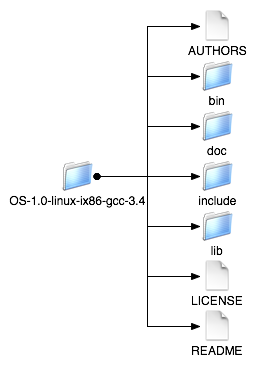
\includegraphics[scale=0.7]{\figurepath/osbinDistribution.png}
\caption{The OS  binary distribution.}
\label{figure:osbindistribution}
\end{figure}

In the {\tt java} directory  are the binary files required to build an Apache Tomcat-based Web service that will take SOAP envelopes with model instances in OSiL format and/or options in OSoL format, call the {\tt OSSolverService}, and return the optimization result in OSrL format.  This distribution is named
\begin{verbatim}
os-distribution-release_number.zip
\end{verbatim}
and the details and use of this distribution are described in Section \ref{section:tomcat}.



\section{Building and Testing the OS Project}\label{section:build}


Once the OS source code is obtained, the OS libraries, {\tt OSSolverService} executable, and test examples can be built.  We describe how to do this on Unix/Linux systems (see Section \ref{section:unixbuilds})  and on Windows (see Section \ref{section:windowsintall}).

\subsection{Building the OS Project on Unix/Linux Systems}\label{section:unixbuilds}

In order to build the OS project on Unix/Linux systems do the following.

\vskip 8pt


\noindent {\bf Step 1:}  Make and connect to the distribution root directory.

\begin{verbatim}
mkdir COIN-OS
cd COIN-OS
\end{verbatim}


\noindent {\bf Step 2:} Run the configure script that will generate the makefiles.  If you are running on a machine with a FORTRAN 95 compiler present (e.g. {\tt gfortran}) run the command

\begin{verbatim}
./configure
\end{verbatim}

\noindent otherwise for now use

\begin{verbatim}
./configure  COIN_SKIP_PROJECTS=Ipopt
\end{verbatim}
as COIN-OR's Ipopt project currently uses Fortran to compile some of its dependent libraries.

\vskip 8pt
\noindent {\bf Note:}

\begin{itemize}
\item If {\tt gfortran} is not present and you  wish to build the nonlinear solver {\tt Ipopt} see the instructions in Section \ref{section:ipopt}.

\item When using {\tt configure} you may wish to use the {\tt -C} option. This   instructs configure to use a cache file, {\tt config.cache}, to speed up configuration by remembering and reusing the results of tests already performed.

\item For more information and options on the {\tt ./configure} script see


\url{https://projects.coin-or.org/BuildTools/wiki/user-configure#PreparingtheCompilation}.


\end{itemize}



\noindent {\bf Step 3:}  Run the make files.

\begin{verbatim}
make
\end{verbatim}

\noindent {\bf Step 4:} Run the {\tt unitTest}.

\begin{verbatim}
make test
\end{verbatim}

Depending upon which third party software you have installed, the result of running the unitTest should look something like (we have included the third-party solvers LINDO and Knitro in the  test results below; they are not part of the default build):


{\small
\begin{verbatim}
HERE ARE THE UNIT TEST RESULTS:

Solved problem avion2.osil with Ipopt
Solved problem HS071.osil with Ipopt
Solved problem rosenbrockmod.osil with Ipopt
Solved problem parincQuadratic.osil with Ipopt
Solved problem parincLinear.osil with Ipopt
Solved problem callBack.osil with Ipopt
Solved problem callBackRowMajor.osil with Ipopt
Solved problem parincLinear.osil with Clp
Solved problem p0033.osil with Cbc
Solved problem rosenbrockmod.osil with Knitro
Solved problem callBackTest.osil with Knitro
Solved problem parincQuadratic.osil with Knitro
Solved problem HS071_NLP.osil with Knitro
Solved problem p0033.osil with SYMPHONY
Solved problem parincLinear.osil with DyLP
Solved problem volumeTest.osil with Vol
Solved problem p0033.osil with GLPK
Solved problem lindoapiaddins.osil with Lindo
Solved problem rosenbrockmod.osil with Lindo
Solved problem parincQuadratic.osil with Lindo
Solved problem wayneQuadratic.osil with Lindo
Test the MPS -> OSiL converter on parinc.mps usig Cbc
Test the AMPL nl -> OSiL converter on hs71.nl using LINDO
Test a problem written in b64 and then converted to OSInstance
Successful test of OSiL parser on problem parincLinear.osil
Successful test of OSrL parser on problem parincLinear.osrl
Successful test of prefix and postfix conversion routines on problem rosenbrockmod.osil
Successful test of all of the nonlinear operators on file testOperators.osil
Successful test of AD gradient and Hessian calculations on problem CppADTestLag.osil


CONGRATULATIONS! YOU PASSED THE UNIT TEST
\end{verbatim}
}

If you do not see
\begin{verbatim}
CONGRATULATIONS! YOU PASSED THE UNIT TEST
\end{verbatim}
then you have not passed the unitTest and hopefully some semi-inteligble error message was given.

\vskip 8pt

\noindent {\bf Step 5:}  Install the libraries and executables.  In addition you will have the following directories.

\begin{verbatim}
make install
\end{verbatim}

This will install all of the libraries in the {\tt lib} directory.  In particuar, the main OS library {\tt libOS} along with the libraries of the other COIN-OR project that download with the OS project will get installed in the {\tt lib} directory.  In addtion the {\tt make install} command will install four executable programs in the {\tt bin} directory.  One of these binaries is {\tt OSSolverService} which is main OS project executable. This is described in Section \ref{section:ossolverservice}. In addition {\tt clp}, {\tt cbc}, {\tt ipopt}, and {\tt symphony} get installed  in the {\tt bin} directory.  Necessary header files are installed in the {\tt include} directory.   In this case, {\tt bin}, {\tt lib}, and {\tt include} are all subdirectories of where {\tt ./configure} is run.   If the user wants these files installed elsewhere, then configure should specify the {\tt prefix} of these directories.  That is,


\begin{verbatim}
./configure  --prefix=prefixDirctory  COIN_SKIP_PROJECTS=Ipopt
\end{verbatim}

For example, running

\begin{verbatim}
./configure  --prefix=/usr/local  COIN_SKIP_PROJECTS=Ipopt
\end{verbatim}

\noindent and then running {\tt make} and {\tt make install} will put the relevant files in

\begin{verbatim}
/usr/local/bin
/usr/local/include
/usr/local/lilb
\end{verbatim}

\vskip 8pt

{\bf Run an Example!}  If {\tt make test} works, proceed to Section \ref{section:ossolverservice} to run the key executable, {\tt OSSolverService}.







\subsection{Building the OS Project on Windows}\label{section:windowsintall}

There are a number of options open to Windows users.   First, if you wish to work with source code we recommend downloading  the svn client,  TortoiseSVN.  See \url{tortoisesvn.tigris.org}.  With TortoiseSVN in the Windows Explorer connect to the directory (e.g. COIN-OS) where you wish to put the OS code. Right click on the directory and select {\tt SVN Checkout}.   In the textbox, {\tt URL of Repository} give the URL for the version of the OS project you wish to checkout, e.g. https://projects.coin-or.org/svn/OS/stable/1.0.

Also, if you plan to build any of the projects contained in {\tt ThirdParty} (e.g. ASL) we recommend using {\tt wget}.  The {\tt wget} executable is used by the scripts, {\tt get.ASL}, {\tt get.Blas}, etc. in the corresponding third party subdirectories and makes it easy to download the software.  A Windows version of {\tt wget} is available at

\begin{verbatim}
http://www.christopherlewis.com/WGet/WGetFiles.htm
\end{verbatim}



\subsubsection{Microsoft Visual Studio}

Microsoft Visual Studio solution files are provided for users of Windows and the Microsoft Visual Studio IDE.     It is assumed that the user has installed a copy of Microsoft Visual Studio.  Users interested in a Visual Studio build of the OS project can obtain Visual C++ 2008 Express Edition for free at \url{http://msdn2.microsoft.com/en-us/express/future/bb421473.aspx}.  This download will include the Microsoft {\tt cl}  C++ compiler along with necessary libraries.




There is a directory {\tt MSVisualStudio} in the {\tt COIN-OS/OS}  directory.  The {\tt MSVisualStudio} contains root directories organized by the version of Visual Studio.  We currently provide solution files  for Version 7 and Version 8.  There are project files for building the unitTest ({\tt OSTest.vcproj}),  the OSSolverService ({\tt OSSolverService.vcproj}), and the OS library {\tt libOS.vcproj}.   The Microsoft Visual Studio files are automatically downloaded with an SVN checkout. They are also contained in the tarballs.  See Section \ref{section:getTarBalls}.

\vskip 8pt


{\bf Important Note For  Users of Visual Studio Express:}  The part of the OS library responsible for communication with a remote server depends on some underlying Windows socket header files and libraries. If you are using the Visual Studio Express Edition, these files are not included in the download and it is necessary  to also download and install the Windows Platform SDK. Download the necessary files at
 \url{http://msdn2.microsoft.com/en-us/express/aa700755.aspx}

{\bf Important Note for Running Executables:}  There are two projects that build executable files. These are {\tt OSTest} and {\tt OSSolverService}. These executable files are located in the {\tt Debug} directory that is the Visual Studio project root. These must be moved to the appropriate directories.   The {\tt OSTest} executable should be moved to the {\tt COIN-OS/OS/test} directory and the {\tt OSSolverService} executable should be moved to either the {\tt COIN-OS/OS/src} directory or {\tt COIN-OS/OS/bin}.

\subsubsection{Cygwin}

{\tt Cygwin} provides a Unix emulation environment for Windows. It comes with numerous tools and libraries including the gcc compilers. See {\tt www.cygwin.com}.   Cygwin can be used the Gnu Compiler Collection (gcc) or with the Microsoft {\tt cl} compiler.


{\bf Using Cygwin with gcc:}  With Cygwin and the corresponding gcc compilers the OS project is  built exactly as described in Section \ref{section:svn}. If you have previously downloaded Cygwin with version gnome make version 3.81-1,  you must obtain a fixed 3.81 version from \url{http://www.cmake.org/files/cygwin/make.exe}. (See also  the Cygwin mailing list postings \url{http://cygwin.com/ml/cygwin/2006-09/msg00315.html} and \url{http://cygwin.com/ml/cygwin/2006-09/msg00153.html}).  See also the discussion at \url{https://projects.coin-or.org/BuildTools}.


\vskip 8pt

{\bf Using Cygwin with Microsoft cl:}   Users who are extremely adventuresome and have an abundance  of free time on their hands may wish to use Cygwin the Microsoft {\tt cl} compiler to build the OS project.   The following steps have led to a successful build.


\begin{itemize}
\item[Step 1:]  Download {\tt Cygwin}  from \url{http://www.cygwin.com/setup.exe} and install.




\item[Step 2:]   Download  Visual Studio Express C++ at  \url{http://msdn2.microsoft.com/en-us/express/aa975050.aspx}.


 \item[Step 3:]  The part of the OS library responsible for communication with a remote server depends on some underlying Windows socket header files and libraries. Therefore it is necessary to also download and install the Windows Platform SDK. Download the necessary files at

 \url{http://msdn2.microsoft.com/en-us/express/aa700755.aspx}

 and install.



\item[Step 4:]  Set the Cygwin search path configuration. This is important.
This step is necessary to insure that Cygwin   looks for compilers, linkers, etc in the correct order.  The right order of directories  is: MSVS command directories, Cygwin command directories, and finally Windows command directories.  This is illustrated below.

\begin{itemize}

 \item First, Cygwin should look in the Microsoft Visual Studio directories.  If a standard Visual Studio install is done, the following  should part of the Cygwin search path

\begin{verbatim}
.
:/cygdrive/c/Program Files/Microsoft Visual Studio 8/Common7/IDE
:/cygdrive/c/Program Files/Microsoft Visual Studio 8/VC/bin
:/cygdrive/c/Program Files/Microsoft Visual Studio 8/Common7/Tools
:/cygdrive/c/Program Files/Microsoft Visual Studio 8/SDK/v2.0/Bin
:/cygdrive/c/Program Files/Microsoft Visual Studio 8/VC/vcpackages
:/cygdrive/c/WINDOWS/Microsoft.NET/Framework/v2.0.50727
\end{verbatim}

\item Second, Cygwin should next search its  command directories.  The following is typical of a standard install.

\begin{verbatim}
/bin:/usr/local/bin:/usr/bin:/bin:/usr/X11R6/bin
\end{verbatim}

\item Third, Cygwin should search the Windows specific command directories.  The following is typical.

{\tiny
\begin{verbatim}
:/cygdrive/c/WINDOWS/system32:/cygdrive/c/WINDOWS
:/cygdrive/c/WINDOWS/System32/Wbem:/cygdrive/c/Program Files/ATI Technologies/ATI Control Panel
:/cygdrive/c/Program Files/Common Files/Roxio Shared/DLLShared/
:/cygdrive/c/Program Files/QuickTime/QTSystem/:/cygdrive/c/Program Files/Microsoft SQL Server/90/Tools/binn/
:/cygdrive/c/Program Files/Microsoft Platform SDKfor Windows Server 2003 R2/Bin/
:/cygdrive/c/Program Files/Microsoft Platform SDK for Windows Server 2003 R2/Bin/WinNT/
:/cygdrive/c/Program Files/SSH Communications Security/SSH Secure Shell
:/cygdrive/c/Program Files/Microsoft Platform SDK for Windows Server 2003 R2/Bin/
:/cygdrive/c/Program Files/Microsoft Platform SDK for Windows Server 2003 R2/Bin/WinNT/
:/cygdrive/d/SSH
\end{verbatim}
}


\end{itemize}
Open the Cygwin shell and check the value of {\tt \$PATH}. If directories don't appear in an order described above, then  {\tt \$PATH} value needs to be reset.

\item [Step 5:] This step is necessary only if you wish to build with the AMPL {\tt ASL} solver library.   Unfortunately, and we regret this, but at the time of this writing the working version of ASL for cygwin/cl build is its trunk version. This means that it is necessary to download the trunk version separately and replace the release version we have distributed with the trunk version.  The URL for the trunk version is

\begin{verbatim}
co https://projects.coin-or.org/svn/BuildTools/ThirdParty/ASL/trunk  ASL
\end{verbatim}





\item [Step 6:] Build the OS project (or any COIN-OR project). If you wish to avoid the FORTRAN related issues you should build without Ipopt. Issue the following command in the project root.
\begin{verbatim}
./configure COIN_SKIP_PROJECTS=Ipopt --enable-doscompile=msvc
\end{verbatim}

If you wish to build with Ipopt, then FORTRAN is required and Visual Studio does not ship with FORTRAN compiler. The following is a work-around.

\begin{itemize}

\item[Step a.]  Obtain one of the   Harwell Subroutine Library (HSL) routines {\tt ma27ad.f} or {\tt MA57ad.f}.  See \url{http://www.cse.scitech.ac.uk/nag/hsl/}.  Put the Harwell code in the directory {\tt ThirdParty/HSL}.




\item[Step b.]  Follow the instructions for downloading and installing {\tt f2c} compiler from Netlib.  The installation instructions for this are in the {\tt INSTALL} file in
\begin{verbatim}
../data/BuildTools/compile_f2c
\end{verbatim}



\item[Step c.]  Run configure

\begin{verbatim}
 ./configure  --enable-doscompile=msvc
 \end{verbatim}


\end{itemize}


\end{itemize}

\subsubsection{MinGW}



MinGW (Minimalist GNU for Windows) is set of runtime headers to be used with the GNU gcc compilers for Windows.  See \url{www.mingw.org}. As with Cygwin, the OS project is  built exactly as described in Section \ref{section:svn}.

\subsubsection{MSYS}



MSYS (Minimal SYSstem) provides an easy way to use the COIN-OS build system with compilers/linkers of your own choice, such as the Microsoft command line C++ cl compiler.  MSYS is an application that gives the user a Bourne shell that can run {\tt configure}  scripts and {\tt Makefiles}.  No compilers come with MSYS. In the Cygwin, MinGW, and MSYS hierarchy, it is at the bottom in terms of tools provided. However, it is very easy to use and build the OS project with MSYS.    In this discussion we assume that the user has downloaded the OS source code (most likely  with Tortise) and that the {\tt cl} compiler is present.  The project is built using the following steps.

\vskip 8pt

\noindent {\bf Note:}

\begin{itemize}

\item If you wish to use the third-party software with MSYS it is best to get {\tt wget}. See \ref{section:windowsintall}.

 \item Do not put any imbedded blanks in the path to the OS project.
 \end{itemize}



Execute the following steps to use the Microsoft C++ cl compiler with MSYS.


\begin{itemize}

\item[Step 1.] Download {\tt MSYS} at

\begin{center}
\url{http://sourceforge.net/project/showfiles.php?group_id=2435&package_id=24963}
\end{center}

and install.  Double clicking on the MSYS icon will open a Bourne shell window.

\item[Step 2.]  Download  Visual Studio Express C++ at

 \url{http://msdn2.microsoft.com/en-us/express/future/bb421473.aspx}

and install.

 \item[Step 3.]  The part of the OS library responsible for communication with a remote server depends on some underlying Windows socket header files and libraries. Therefore it is necessary to also download and install the Windows Platform SDK. Download the necessary files at

 \url{http://msdn2.microsoft.com/en-us/express/aa700755.aspx}

 and install.

\item[Step 4.]   Set the Visual Studio environment variables so that paths to the necessary libraries and header files  are recognized.  Assuming that a standard installation was done for the Visual Studio Express and the Windows Platform SDK set the variables as follows:

\begin{verbatim}
PATH=C:\Program Files\Microsoft Visual Studio 8\Common7\IDE;
C:\Program Files\Microsoft Visual Studio 8\VC\BIN;
C:\Program Files\Microsoft Visual Studio 8\Common7\Tools;
C:\Program Files\Microsoft Visual Studio 8\SDK\v2.0\bin;
C:\WINDOWS\Microsoft.NET\Framework\v2.0.50727;
C:\Program Files\Microsoft Visual Studio 8\VC\VCPackages


INCLUDE=C:\Program Files\Microsoft Visual Studio 8\VC\INCLUDE;
C:\Program Files\Microsoft Platform SDK for Windows Server 2003 R2\Include

LIB = C:\Program Files\Microsoft Visual Studio 8\VC\LIB;
C:\Program Files\Microsoft Visual Studio 8\SDK\v2.0\lib;
C:\Program Files\Microsoft Platform SDK for Windows Server 2003 R2\Lib
\end{verbatim}

The environment variables can be set using the {\tt System Properties} in the Windows {\tt Control Panel}.


\item[Step 5.]  In the MSYS command window connect to the root of the OS project and run  {\tt configure}  script  and then {\tt make} as described in Section \ref{section:unixbuilds}.

\end{itemize}






{\bf Run an Example!}  If {\tt make test} works, proceed to Section \ref{section:ossolverservice} to run the key executable, {\tt OSSolverService}.








\subsection{VPATH Installations}


It is possible to build the OS project in a directory that is different from the directory where the source code is present. This is called a {\tt VPATH}  compiliation.  A {\tt VPATH}  compilation  is very useful if you wish to build several versions (e.g. debug and non-debug version, or versions with various combinations of third-party software available) of the OS project from a single copy the source code.

For  example, assume you wish to build a debug version of the OS project in the directory {\tt vpath-debug} and that the environment variable {\tt OS} is the path to the root of the OS project distribution {\tt COIN-OS}.  Connect to the {\tt vpath-debug} directory run configure as follows (assuming we do want a debug version)

\begin{verbatim}
../COIN-OS/configure --enable-debug
\end{verbatim}

After you run configure, the OS project directory structure will be present in the {\tt vpath-debug} directory along with all of the necessary  {\tt Makefiles}.  Next inside the {\tt vpath-degug} execute

\begin{verbatim}
make
\end{verbatim}

and all of  the libraries created will be in their respective directories inside {\tt vpath-debug}  and not {\tt COIN-OS}.

\vskip 8pt
\noindent {\bf Note:} If you have run the {\tt configure} script inside the {\tt COIN-OS} directory, you cannot do a {\tt VPATH} build. Before doing a {\tt VPATH} build you need to run
\begin{verbatim}
make distclean
\end{verbatim}
in the {\tt COIN-OS} directory.


\subsection{Using Ipopt}\label{section:ipopt}


Ipopt is a COIN-OR project (\url{projects.coin-or.org/Ipopt}) and is included in the download with the OS project. However, unlike the other COIN-OR projects that download with OS, the Ipopt project requires third-party software that is based on FORTRAN and care must be taken if you wish to build OS with the  Ipopt solver.  You can  exclude Ipopt from the OS  build by adding the option

\begin{verbatim}
COIN_SKIP_PROJECTS=Ipopt
\end{verbatim}
to the {\tt configure} script.


If you do choose to build Ipopt, first get the necessary third-party software.  First connect into the {\tt ThirdParty} directory. Then execute the following commands:

\begin{verbatim}
$ cd /Blas
$ ./get.Blas
$ cd ../Lapack
$ ./get.Lapack
$ cd ../Mumps
$ ./get.Mumps
\end{verbatim}

Alternatively, you can connect into the project root {\tt COIN-OS} and execute the script {\tt get.AllThirdParty}.  This will also get the AMPL {\tt ASL} libraries.

What you do next depends upon whether or not a FORTRAN compiler is present, and if so, which version of FORTRAN.  There are three options.

\begin{itemize}

\item[Option 1.]   If you are building in Unix-like environment and have a FORTRAN 95 compiler available, you can simply run the {\tt configure} script and the FORTRAN compiler will be detected and the {\tt Ipopt} project will be built.

\item[Option 2.]   If you have a FORTRAN 77 compiler, you  must first obtain one of the   Harwell Subroutine Library (HSL) routines {\tt ma27ad.f} or {\tt MA57ad.f}.  See \url{http://www.cse.scitech.ac.uk/nag/hsl/}.  Put the Harwell code in the directory {\tt \../data/ThirdParty/HSL}.  Now run the {\tt configure} script as described in \ref{section:svn}.  See

\begin{verbatim}
 http://www.coin-or.org/Ipopt/documentation/node15.html
 \end{verbatim}

\item[Option 3.]  If you do not have a FORTRAN compiler and do not wish to obtain one, you can use the {\tt f2c} compiler from Netlib.  The installation instructions for this are in the {\tt INSTALL} file in
\begin{verbatim}
../data/BuildTools/compile_f2c
\end{verbatim}

\end{itemize}

\noindent Two important points:


\begin{itemize}
\item Option 3 also requires that  one of the  Harwell Subroutine Library (HSL) routines {\tt ma27ad.f} or  {\tt MA57ad.f} be present in the HSL directory.

\item If you run configure with the {\tt --enable-debug} option on Windows, then when building the {\tt vcf2c.lib}, use the command line

\begin{verbatim}
CFLAGS = -MTd -DUSE_CLOCK -DMSDOS -DNO_ONEXIT
\end{verbatim}

\end{itemize}





\subsection{Third-Party Software}

By third-party software we mean software not available for download at \url{www.coin-or.org}. The default OS project is configured out-of-the-box with the COIN-OR  projects {\tt Cbc}, {\tt Clp}, {\tt Cgl}, {\tt CoinUtils}, {\tt CppAD},  {\tt DyLP}, {\tt SYMPHONY}, and {\tt Vol}.  However, the project is also designed to work with other COIN-OR projects and several other open source and commercial software projects.

In many of the header files there are {\tt \#include} statements inside {\tt  \#ifdef}  statements. For example,
\begin{verbatim}
#ifdef COIN_HAS_LINDO
#include "LindoSolver.h"
#endif
#ifdef COIN_HAS_IPOPT
#include "IpoptSolver.h"
#endif
\end{verbatim}
In the {\tt inc} subdirectory of the {\tt OS}  directory, there is a header file, {\tt config\_os.h} that defines the values of the
\begin{verbatim}
COIN_HAS_XXXXX
\end{verbatim}
variables. If the project is configured with the simple {\tt ./configure} command given in Step 3 with no arguments, then in the {\tt config\_os.h} these variables associated with the third-party software will be undefined. For example.
\begin{verbatim}
/* Define to 1 if the Cplex package is used */
/* #undef COIN_HAS_CPX */
\end{verbatim}
unlike the configured COIN-OR projects that appear as
\begin{verbatim}
/* Define to 1 if the Clp package is used */
#define COIN_HAS_CLP 1
\end{verbatim}
In the following subsections we  describe how to incorporate various  third-party packages into the OS project and see to it that the
\begin{verbatim}
COIN_HAS_XXXXX
\end{verbatim}
variable is defined in  {\tt config\_os.h}.

\subsubsection{AMPL}

The OS library contains a class, {\tt OSnl2osil} (see Section (\ref{section:nl2osil}) ) and {\tt amplClient} (see Section (\ref{section:amplclient}) ) that require the use of the AMPL ASL library.  See \url{http://netlib.sandia.gov/ampl/}  and  \url{http://www.ampl.com}. Users with a Unix system should locate the {\tt ASL} folder that is part of the distribution. The {\tt ASL} folder is in the {\tt ThirdParty} folder which is in the project root folder. Locate and execute the {\tt get.ASL} script.  Do this prior to running the {\tt configure} script. The {\tt configure} script will build the correct ASL library.

Microsoft  Visual Studio users will have to build the ASL library separately and then link it with the OS lib in the OS project file.  The necessary source files are at
\begin{verbatim}
http://netlib.sandia.gov/cgi-bin/netlib/netlibfiles.tar?filename=netlib/ampl/solvers
\end{verbatim}
 After unpacking the distribution build the source code with the utility {\tt nmake} which should be part of the Visual Studio distribution. The appropriate command is
\begin{verbatim}
nmake -f makefile.vc
\end{verbatim}
If the OS project is properly configured  with the ASL library, {\tt config\_os.h} will contain the lines
\begin{verbatim}
/* If defined, the Ampl Solver Library is available. */
#define COIN_HAS_ASL 1
\end{verbatim}

At this point the reader may wish to view
\begin{verbatim}
https://projects.coin-or.org/BuildTools/wiki/user-configure#CommandLineArgumentsforconfigure
\end{verbatim}
for more information on command line arguments that are illustrated in the subsections below.


\subsubsection{Cplex}

Cplex is a linear, integer, and quadratic solver. See \url{http://www.ilog.com/products/cplex/}.  Cplex does not provide source code and you can only download the platform dependent binaries. After installing the binaries and include files in an appropriate directory, run configure to point to the include and library directory. An example is given below:

\begin{verbatim}
configure --with-cplex-lib="-L$(CPLEXDIR)/lib/$(SYSTEM)/$(LIBFORMAT)
 $(CPLEX_LIBS)" --with-cplex-incdir= $(CPLEXDIR)/include
\end{verbatim}

You may also need the following environment variables (if they are not already set). The following are values we used in a working implementation.
\begin{verbatim}
SYSTEM =i86_linux2_glibc2.3_gcc3.2
LIBFORMAT =static_pic_mt
CPLEXDIR =/usr/local/ilog/cplex81/include/ilcplex
CPLEXLIBPATH= -L$(CPLEXDIR)/lib/$(SYSTEM)/$(LIBFORMAT)
CPLEXINCDIR = $(CPLEXDIR)/include
CPLEX_LIBS=-lcplex -lilocplex -lm -lpthread
ILOG_HOME=/usr/local/ilog/cplex81/bin/i86_linux2_glibc2.3_gcc3.2
ILOG_LICENSE_FILE=/usr/local/ilog/ilm/access.ilm
PATH=***:/usr/local/ilog/cplex81/bin/i86_linux2_glibc2.3_gcc3.2:***
CLASSPATH=:/usr/local/ilog/cplex81/bin/i86_linux2_glibc2.3_gcc3.2:
\end{verbatim}

\subsubsection{GLPK}

{\tt GLPK} is a an open-source linear and integer-programming solver from the GNU organization. See \url{http://www.gnu.org/software/glpk/}.  In order to use GLPK with OS, either execute {\tt get.AllThirdParty} or connect to {\tt ThirdParty/Glpk} and execute {\tt get.ThirdParty}.










\subsubsection{Knitro}


Knitro is a nonlinear solver. See \url{http://www.ziena.com/}.  Ziena does not provide source code for Knitro.  You must download platform dependent binaries.   In order to use Knitro with the OS project, perform the following steps.

\begin{itemize}



\item[Step 1:]  Download {\tt knitro} to the desired directory.


\item[Step 2:] Copy the file {\tt nlpProblemDef.h} from the {\tt examples/C++} directory to the {\tt include} directory.

\item[Step 3:]  Edit the file {\tt nlpProblemDef.h} and delete the following lines:

\begin{verbatim}
NlpProblemDef::~NlpProblemDef (void)
{
    //---- DO NOTHING.
    return;
}
\end{verbatim}




\item[Step 4] Run configure with appropriate values for  {\tt --with-knitro-lib} and {--with-knitro-incdir}. For example:

\begin{verbatim}
./configure --with-knitro-lib="-L/home/kmartin/files/code/knitro/linux/lib -lknitro "
--with-knitro-incdir=/home/kmartin/files/code/knitro/linux/include
\end{verbatim}

\end{itemize}


\subsubsection{LINDO}

LINDO is a commercial linear, integer, and nonlinear solver. See \url{www.lindo.com}.  LINDO does not provide source code and you can only download the platform dependent binaries. After installing the binaries and include files in an appropriate directory, run configure to point to the include and library directory. An example is given below:

\begin{verbatim}
--with-lindo-lib="-L/home/kmartin/files/code/lindo/linux/lib -llindo -lmosek"
--with-lindo-incdir=/home/kmartin/files/code/lindo/linux/include
\end{verbatim}


\subsubsection{MATLAB}

Install MATLAB on the client machine and follow the instruction in Section
 \ref{section:usingmatlab}.

\subsubsection{Library Paths}

After running {\tt configure} as described above,  on Unix systems, it will be necessary to set the environment variables {\tt LD\_LIBRARY\_PATH} or {\tt DYLD\_LIBRARY\_PATH} (on Mac OS X) to point to the location of the installed third party libraries in the case that the libraries are dynamic and not static libraries.


\subsection{Bug Reporting}

Bug reporting is done through the project Trac page. This is at
\begin{verbatim}
http://projects.coin-or.org/OS
\end{verbatim}
To report a bug, you must be a registered user.  For  instructions on  how to register, go to
\begin{verbatim}
http://www.coin-or.org/usingTrac.html
\end{verbatim}
After registering, log in and then file a trouble ticket by going to
\begin{verbatim}
http://projects.coin-or.org/OS/newticket
\end{verbatim}


\subsection{Documentation}\label{section:documentation}

If you have Doxygen  (\url{www.doxygen.org}) available (the executable {\tt doxygen} should be in the {\tt path} command) then executing
\begin{verbatim}
make doxydoc
\end{verbatim}
in the project root directory will result in the Doxygen documentation being generated and stored in the {\tt doxydoc} folder in the project root.

In order to view the documentation, open a browser and open the file
\begin{verbatim}
projectroot/doxydoc/html/index.html
\end{verbatim}

Running Doxygen will generate documentation for only the  OS project.  Documentation will not be generated for the other COIN-OR projects in the project root. In the {\tt doxydoc}  folder is a configuration file {\tt doxygen.conf}.  This configuration file contains the {\tt EXCLUDE} parameter

\begin{verbatim}
EXCLUDE =  Cbc \
   Cgl \
   Clp \
   CoinUtils \
   cppad \
   SYMPHONY \
   Vol \
   DyLP \
   ThirdParty \
   Osi \
   include
\end{verbatim}

This file can be edited, and any project for which documentation is desired, can be deleted from the {\tt EXCLUDE} list.






\subsection{Platforms}

The build process described in Section \ref{section:svn} has been tested on Linux, Mac OS X, and on Windows using  MINGW/MSYS and CYGWIN. The  gcc/g++ and Microsoft  cl compiler have been tested. A number of solvers have also been tested with the OS library. For a list of tested solvers and platforms see Table \ref{table:testedplatforms}.  More detail on the platforms listed in Table  \ref{table:testedplatforms} is given in Table \ref{table:platformdescription}.


\begin{table}
\caption{Tested Platforms for Solvers}
\centering
\label{table:testedplatforms}
\vskip 8pt
 \begin{tabular}{l|c|c|c|c|c|c|}
 &Mac&Linux&Cyg-gcc&Msys-cl&MinGW-gcc&MSVS \\ \hline
AMPL-Client &x&x&&x&& \\ \hline
MATLAB &x&&&&& \\ \hline
Cbc &x&x&x&x&x&x \\ \hline
Clp &x&x&x&x&x&x \\ \hline
Cplex &&x&&&& \\ \hline
DyLP &x&x&x&x&x&x \\ \hline
Ipopt &x&x&x&x&& \\ \hline
Knitro &x&x&&&& \\ \hline
Lindo &x&x&&x&&x \\ \hline
SYMPHONY &x&x&x&x&x&x \\ \hline
Vol &x&x&x&x&x&x \\ \hline
\end{tabular}
\end{table}


 \begin{table}
\caption{Platform Description}
\centering
\label{table:platformdescription}
\vskip 8pt
 \begin{tabular}{l|c|c|c|}
 & {\bf Operating System} & {\bf Compiler} & {\bf  Hardware} \\ \hline
 Mac &Mac OS X 10.4.9&gcc 4.0.1&Power PC \\   \hline
  Mac &Mac OS X 10.4.10&gcc 4.0.1&Intel \\   \hline
 Linux &Red Hat 3.4.6-8&gcc 3.4.6& Dell Intel 32 bit chip\\ \hline
 Cyg-gcc &Windows 2003 Server&gcc 3.4.4& Dell Intel 32 bit chip \\ \hline
 Msys-cl &Windows XP&Visual Studio 2003 &Dell Intel 32 bit chip \\ \hline
 MinGW-gcc &Windows XP&gcc 3.4.2&Dell Intel 32 bit chip \\ \hline
 MSVS &Windows XP&Visual Studio 2003 &Dell Intel 32 bit chip \\ \hline
\end{tabular}
\end{table}


\section{The OS Project Components}\label{section:projectcomponents}

The directories in the  project root  are outlined in Figure  \ref{figure:osprojectrootdir}.

If you download the OS package, you get these additional COIN-OR projects. The links to the project home pages are provided below and give more information on these projects.
\begin{itemize}
\item {\tt BuildTools} - \url{projects.coin-or.org\BuildTools}
\item {\tt Cbc} - \url{projects.coin-or.org\Cbc}
\item {\tt Cgl} - \url{projects.coin-or.org\Cgl}
\item {\tt Clp}  - \url{projects.coin-or.org\Clp}
\item {\tt CoinUtils} - \url{projects.coin-or.org\CoinUtils}
\item {\tt CppAD} - \url{projects.coin-or.org\CppAD}
\item {\tt Dylp} - \url{projects.coin-or.org\Dylp}
\item {\tt Ipopt} - \url{projects.coin-or.org\Ipopt}
\item {\tt Osi} - \url{projects.coin-or.org\Osi}
\item {\tt SYMPHONY}   - \url{projects.coin-or.org\SYMPHONY}
\item {\tt Vol}   - \url{projects.coin-or.org\Vol}
\end{itemize}

The following directories are also in the project root.
\begin{itemize}
\item {\tt bin} - after executing {\tt make install} the bin directory will contain {\tt OSSolverService}, {\tt clp}, {\tt cbc},  {\tt cbc-generic} and {\tt symphony}.

\item {\tt Data} - this directory contains numerous test problems that are used by some of the COIN-OR project's unitTest.

\item {\tt doxydoc} - is a folder for documentation.

\item {\tt include} - is a directory for header files. If the user wishes to write code to link against any of the libraries in the {\tt lib} directory, it may be necessary to include these header files.

\item {\tt lib} - is a directory of libraries. After running {\tt make install} the OS library along with all other COIN-OR libraries are installed in {\tt lib}.

\item {\tt ThirdParty} - is a  directory for third party software. For example, if AMPL related software is used such as {\tt amplClient} is used, then certain AMPL libraries need to be present. This should go into the {\tt ASL} directory in {\tt ThirdParty.}
\end{itemize}


The directories in the OS directory are outlined in Figure \ref{figure:osdirectory}.


\begin{figure}
\centering
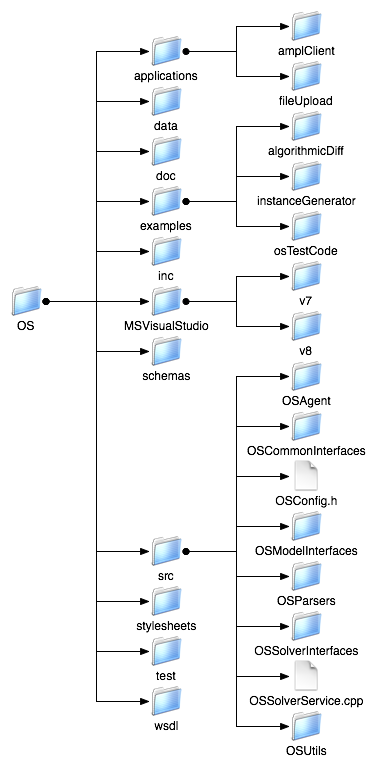
\includegraphics[scale=0.8]{\figurepath/OSDirectory.png}
\caption{The OS directory.}
\label{figure:osdirectory}
\end{figure}

The OS directories include the following:

\begin{itemize}

\item {\tt data} - is a directory that holds test problems. These test problems are used by the {\tt unitTest}. Many of these files are also used to illustrate how the {\tt OSSovlerService} works. See Section \ref{section:ossolverservice}.

\item {\tt doc} - is the directory with documentation, include this {\it OS User's Manual.}

\item {\tt examples} - is a directory with code examples that illustrate various aspects of the OS project.    These are described in Section \ref{section:examples}.

\item {\tt inc} - is the directory with the config\_os.h file which has information about which projects are included in the distribution.

\item {\tt m4} - is a directory that  contains macro scripts written in the m4 language for auto configuration.

\item {\tt MSVisualStudio} - is a directory that  contains solution files for the Microsoft Visual Studio IDE.  The subdirectories are organized by the version of Visual Studio. We currently provide a solution file for Version 7 and 8.

\item {\tt schemas} - is the directory that contains the W3C XSD (see \url{www.w3c.org}) schemas that are behind the OS standards. These are described in more detail in Section \ref{section:schemadescriptions}.

\item {\tt src} - is the directory with all of the source code for the OS Library and for the executable {\tt OSSolverService}. The OS Library components are described in Section \ref{section:oslibrary}.

\item {\tt stylesheets} - this directory contains the XSLT stylesheet that is used to transform the solution instance in OSrL format into HTML so that it can be displayed in a browser.

\item {\tt test} - this directory contains the {\tt unitTest}.


\item  {\tt wsdl} - is a directory of WSDL (Web Services Discovery Language) files. These are used to specify the inputs and outputs for the methods and other invocation details provided by a Web service. The most relevant file for the current version of the OS project is {\tt OShL.wsdl}.  This describes the set of inputs and outputs for the methods implemented in the {\tt OSSolverService}. See Section \ref{section:ossolverservice}.

\end{itemize}


\section{OS Protocols}\label{section:schemadescriptions}



The objective of  (OS) is to provide a set of standards for representing optimization instances, results, solver options, and communication between clients and solvers in a distributed environment using Web Services.  These standards are specified by W3C XSD schemas. The schemas for the OS project are contained in the {\tt schemas} folder under the {\tt OS} root. There are numerous schemas in this directory that are part of the OS standard. For a full description of all the schemas see  Ma \cite{junma2005}.  We briefly discuss the standards most relevant to the current version of the OS project.

\begin{itemize}


\item[] {\bf OSiL (Optimization Services instance Language):} an
XML-based language for representing instances of large-scale
optimization problems including linear programs, mixed-integer programs,
quadratic programs, and very general nonlinear programs.

     OSiL,  stores optimization problem instances as
XML files.  Consider the following problem instance that is a
modification of an example of Rosenbrock \cite{rosenbrock1960}:
%
\begin{alignat}{2}
& \mbox{Minimize} & \quad (1 - x_{0})^{2} + 100(x_{1} - x_{0}^{2})^{2} + 9x_{1} \label{eq:roobj}\\
& \mbox{s.t.} & \quad x_{0} + 10.5 x_{0}^{2} + 11.7 x_{1}^{2} + 3x_{0}x_{1}  &\le 25  \label{eq:ro1}\\
& & \ln(x_{0} x_{1}) + 7.5 x_{0} + 5.25 x_{1} &\ge 10 \label{eq:ro2}\\
& & x_{0}, x_{1} &\ge 0 \label{eq:ro3}
\end{alignat}


There are two continuous variables, $x_{0}$ and $x_{1}$, in this instance, each with a lower bound of 0. Figure~\ref{figure:variableselement} shows how we represent this information in an XML-based OSiL file.  Like all XML files, this is a text file that contains both {\it markup} and {\it data}. In this case there are two types of markup, {\it elements} (or {\it tags}\/) and {\it attributes} that describe the elements. Specifically, there are a {\tt <variables>} element and two {\tt <var>} elements. Each {\tt <var>}
element has attributes {\tt lb}, {\tt name}, and {\tt type} that
describe properties of a decision variable: its lower bound, ``name'', and
domain type.


\begin{figure}[b]
\centering
   \small {\obeyspaces\let =\
\fbox{\tt\begin{tabular}{@{}l@{}}
<variables numberOfVariables="2">\\[\Sb]
    <var lb="0" name="x0" type="C"/>\\[\Sb]
    <var lb="0" name="x1" type="C"/>\\[\Sb]
</variables>\\[\Sb]
\end{tabular} }} \medskip
\caption{The {\tt <variables>} element for the example (1)--(4).}\label{figure:variableselement}
\end{figure}


     To be useful for communication between solvers and modeling
languages, OSiL instance files must conform to a standard.
An XML-based representation standard is imposed
through the use of a {\em W3C XML Schema.} The W3C, or World Wide
Web Consortium (\url{www.w3.org}), promotes standards for
the evolution of the web and for interoperability between web
products.  XML Schema (\url{www.w3.org/XML/Schema}) is one
such standard.  A schema specifies the elements and attributes that
define a specific XML vocabulary. The W3C XML Schema is thus a schema
for schemas; it specifies the elements and attributes for a schema
that in turn specifies elements and attributes for an XML
vocabulary such as OSiL. An XML file that conforms to a
schema is called {\it valid} for that schema.

     By analogy to object-oriented programming, a schema is akin to a header file in C++ that defines the members and methods in a class.  Just as a class in C++ very explicitly describes member and method names and properties, a
schema explicitly describes element and attribute names and properties.

{\small
\begin{figure}[b]
   \small {\obeyspaces\let =\
\makebox[0in][t]{\fbox{\tt\begin{tabular}{@{}l@{}}
<xs:complexType name="Variables">\\[\Sb]
    <xs:sequence>\\[\Sb]
        <xs:element name="var" type="Variable" maxOccurs="unbounded"/>\\[\Sb]
    </xs:sequence>\\[\Sb]
    <xs:attribute name="numberOfVariables"\\[\Sb]
            type="xs:positiveInteger" use="required"/>\\[\Sb]
</xs:complexType>\\[\Sb]
\end{tabular} }}} \medskip
\caption{The {\tt  Variables} complexType  in the OSiL
schema.}\label{figure:osilvariables}
\end{figure}
}%end small


{\small
\begin{figure}[b]
   \small {\obeyspaces\let =\
\makebox[0in][t]{\fbox{\tt\begin{tabular}{@{}l@{}}
<xs:complexType name="Variable">\\[\Sb]
    <xs:attribute name="name" type="xs:string" use="optional"/>\\[\Sb]
    <xs:attribute name="init" type="xs:string" use="optional"/>\\[\Sb]
    <xs:attribute name="type" use="optional" default="C">\\[\Sb]
        <xs:simpleType>\\[\Sb]
            <xs:restriction base="xs:string">\\[\Sb]
                <xs:enumeration value="C"/>\\[\Sb]
                <xs:enumeration value="B"/>\\[\Sb]
                <xs:enumeration value="I"/>\\[\Sb]
                <xs:enumeration value="S"/>\\[\Sb]
            </xs:restriction>\\[\Sb]
        </xs:simpleType>\\[\Sb]
    </xs:attribute>\\[\Sb]
    <xs:attribute name="lb" type="xs:double" use="optional" default="0"/>\\[\Sb]
    <xs:attribute name="ub" type="xs:double" use="optional" default="INF"/>\\[\Sb]
</xs:complexType>\\[\Sb]
\end{tabular} }}} \medskip
\caption{The {\tt  Variable} complexType in the OSiL
schema.}\label{figure:osilvar}
\end{figure}
} %end small



Figure ~\ref{figure:osilvariables} is a piece of our schema for OSiL. In W3C XML Schema jargon, it defines a {\it complexType,}  whose purpose is to specify elements and attributes that are allowed to appear in a valid XML instance file such as the one excerpted in Figure~\ref{figure:variableselement}. In particular, Figure~\ref{figure:osilvariables} defines the complexType named {\tt Variables}, which
comprises an element named {\tt <var>} and an attribute named {\tt
numberOfVariables}. The {\tt numberOfVariables} attribute is of a
standard type {\tt positiveInteger}, whereas the {\tt <var>} element is
a user-defined complexType named {\tt Variable}. Thus the complexType {\tt
Variables} contains a sequence of {\tt <var>} elements that
are of complexType {\tt Variable}. OSiL's schema must also provide a
specification for the {\tt Variable} complexType, which is shown in
Figure \ref{figure:osilvar}.

In OSiL the linear part of the problem is stored in the  {\tt
<linearConstraintCoefficients>} element, which stores the coefficient
matrix using three arrays as proposed in the earlier LPFML schema
\cite{fourer2005a}.  There is a child element of {\tt
<linearConstraintCoefficients>} to represent each array: {\tt <value>} for an array of nonzero coefficients, {\tt <rowIdx>} or {\tt <colIdx>} for a corresponding array of row indices or column indices, and {\tt <start>} for an array that indicates where each row or column begins in the previous two arrays.


\begin{figure}[ht]
\centering
   \small {\obeyspaces\let =\
\fbox{\tt\begin{tabular}{@{}l@{}}
<linearConstraintCoefficients numberOfValues="3">\\[\Sb]
    <start>\\[\Sb]
        <el>0</el><el>2</el><el>3</el>\\[\Sb]
    </start>\\[\Sb]
    <rowIdx>\\[\Sb]
        <el>0</el><el>1</el><el>1</el>\\[\Sb]
    </rowIdx>\\[\Sb]
    <value>\\[\Sb]
        <el>1.</el><el>7.5</el><el>5.25</el>\\[\Sb]
    </value>\\[\Sb]
</linearConstraintCoefficients>\\[\Sb]
\end{tabular} }} \medskip\\[\Sb]
\caption{The {\tt <linearConstraintCoefficients>} element for constraints
(\ref{eq:ro1}) and (\ref{eq:ro2}).}\label{figure:rolistMatrix}
\end{figure}

The quadratic part of the problem is represented as follows.

\begin{figure}[ht]
\centering
   \small {\obeyspaces\let =\
\fbox{\tt\begin{tabular}{@{}l@{}}
<quadraticCoefficients numberOfQuadraticTerms="3">\\[\Sb]
     <qTerm idx="0" idxOne="0" idxTwo="0" coef="10.5"/>\\[\Sb]
     <qTerm idx="0" idxOne="1" idxTwo="1" coef="11.7"/>\\[\Sb]
     <qTerm idx="0" idxOne="0" idxTwo="1" coef="3."/>\\[\Sb]
</quadraticCoefficients>\\[\Sb]
\end{tabular} }} \medskip
\caption{The {\tt <quadraticCoefficients>} element for constraint (\ref{eq:ro1}).}
\label{figure:qterms}
\end{figure}

The nonlinear part of the problem is given in Figure \ref{figure:roobjnlnode}.



{\small
\begin{figure}[t]
\centering
   \small {\obeyspaces\let =\
\fbox{\tt\begin{tabular}{@{}l@{}}
<nl idx="-1">\\[\Sb]
     <plus>\\[\Sb]
          <power>\\[\Sb]
               <minus>\\[\Sb]
                    <number value="1.0"/>\\[\Sb]
                    <variable coef="1.0" idx="0"/>\\[\Sb]
               </minus>\\[\Sb]
               <number value="2.0"/>\\[\Sb]
          </power>\\[\Sb]
          <times>\\[\Sb]
               <power>\\[\Sb]
                    <minus>\\[\Sb]
                         <variable coef="1.0" idx="0"/>\\[\Sb]
                         <power>\\[\Sb]
                              <variable coef="1.0" idx="1"/>\\[\Sb]
                              <number value="2.0"/>\\[\Sb]
                         </power>\\[\Sb]
                    </minus>\\[\Sb]
                    <number value="2.0"/>\\[\Sb]
               </power>\\[\Sb]
               <number value="100"/>\\[\Sb]
          </times>\\[\Sb]
     </plus>\\[\Sb]
</nl>\\[\Sb]
\end{tabular} }} \medskip\\[\Sb]
\caption{The {\tt <nl>} element for the nonlinear part of the objective (\ref{eq:roobj}).}\label{figure:roobjnlnode}
\end{figure}
}



 The complete OSiL representation is given in the Appendix.

\item[] {\bf OSrL (Optimization Services result Language):}  an
XML-based language for representing the solution of large-scale
optimization problems including linear programs, mixed-integer programs,
quadratic programs, and very general nonlinear programs.  As example solution (for the problem given in
 (\ref{eq:roobj})--(\ref{eq:ro3}) ) in OSrL format is given below.

\begin{verbatim}
<?xml version="1.0" encoding="UTF-8"?>
<?xml-stylesheet type = "text/xsl"
    href = "/Users/kmartin/Documents/files/code/cpp/OScpp/COIN-OSX/OS/stylesheets/OSrL.xslt"?>
<osrl xmlns="os.optimizationservices.org"
xmlns:xsi="http://www.w3.org/2001/XMLSchema-instance"
xsi:schemaLocation="os.optimizationservices.org
http://www.optimizationservices.org/schemas/OSrL.xsd">
    <resultHeader>
        <generalStatus type="success"/>
        <serviceName>Solved using a LINDO service</serviceName>
        <instanceName>Modified Rosenbrock</instanceName>
    </resultHeader>
    <resultData>
        <optimization numberOfSolutions="1" numberOfVariables="2" numberOfConstraints="2"
            numberOfObjectives="1">
            <solution objectiveIdx="-1">
                <status type="optimal"/>
                <variables>
                    <values>
                        <var idx="0">0.87243</var>
                        <var idx="1">0.741417</var>
                    </values>
                    <other name="reduced costs" description="the variable reduced costs">
                        <var idx="0">-4.06909e-08</var>
                        <var idx="1">0</var>
                    </other>
                </variables>
                <objectives>
                    <values>
                        <obj idx="-1">6.7279</obj>
                    </values>
                </objectives>
                <constraints>
                    <dualValues>
                        <con idx="0">0</con>
                        <con idx="1">0.766294</con>
                    </dualValues>
                </constraints>
            </solution>
        </optimization>

\end{verbatim}




\item[] {\bf OSoL (Optimization Services option Language):}  an
XML-based language for representing options that get passed to an optimization solver or a hosted optimization solver Web service. It contains both standard options for generic services and extendable option tags for solver-specific directives.

\item[] {\bf OSnL (Optimization Services nonlinear Language):}  The OSnL schema is imported by the OSiL schema and is used to represent the nonlinear part of an optimization instane. This is explained in greater detail in Section \ref{section:osexpressiontreeclass}. Also refer to Figue \ref{figure:roobjnlnode} for an illustration of elements from the OSnL standard.



\item[]   {\bf OSpL (Optimization Services process Language):} is a standard for dynamic process information that is kept by the Optimization Services registry.
It is the result of a {\tt knock} operation. See the example given in Section \ref{section:knock}.

\end{itemize}




\section{The OS Library Components}\label{section:oslibrary}

\subsection{OSAgent}\label{section:osagent}

The {\tt OSAgent}  part of the library is used to facilitate communication with remote solvers. It is not used if the solver is invoked locally (i.e. on the same machine).   There are two key classes in the {\tt OSAgent} component of the OS library. The two classes are {\tt OSSolverAgent} and {\tt WSUtil}.

The {\tt OSSolverAgent} class is used  contact a remote solver service.  For example, assume that {\tt sOSiL} is a string with a problem instance and {\tt sOSoL} is a string with solver options. Then the following code will call a solver service and invoke the {\tt the solve} method.
\begin{verbatim}
OSSolverAgent *osagent;
string serviceLocation = http://gsbkip.chicagogsb.edu/os/OSSolverService.jws
osagent = new OSSolverAgent(  serviceLocation );
string sOSrL = osagent->solve(sOSiL, sOSoL);
\end{verbatim}
Other methods in the {\tt OSSolverAgent} class are {\tt send}, {\tt retrieve}, {\tt getJobID}, {\tt knock}, and {\tt kill}.  The use of these methods is described in Section \ref{section:servicemethods}.



The methods in the {\tt OSSolverAgent} class call methods in the {\tt WSUtil} class that perform such tasks and creating and parsing SOAP messages and making low level socket calls to the server running the solver service. The average user will not use methods in the {\tt WSUtil} class, but they are available to anyone wanting to make socket calls or create SOAP messages.

There is also a method, {\tt fileUpload} in the OSAgentClass that is used to upload files from the hard drive of a client to the server. It is very fast and does not involve SOAP or Web Services. The {\tt fileUpload}  method is illustrated and described in the example code {\tt fileUpload.cpp} described in Section \ref{section:fileupload}.

\subsection{OSCommonInterfaces}

The classes in the OSCommonInterfaces component of the OS library are  used  to read and write files and strings in the OSiL and OSrL protocols. See Section \ref{section:schemadescriptions} for more detail on OSiL, OSrL, and other OS protocols. For a complete listing of all of the files in {\tt OSCommonInterfaces} see the Doxygen documentation in the {\tt doxydoc} folder (see Section \ref{section:schemadescriptions}).  Below we highlight some key classes.





\subsubsection{The OSInstance Class}\label{section:osinstanceclass}

The OSInstance class is the in-memory representation of an optimization instance and is a key class for users of the OS project. This class has an API defined by a collection of {\tt get()} methods for extracting various components (such as bounds and coefficients) from a problem instance, a collection of {\tt set()} methods for modifying or generating an optimization instance, and a collection of {\tt calculate()} methods for function, gradient, and Hessian evaluations.  See Section \ref{section:osinstanceAPI}.  We now describe how to create an {\tt OSInstance} object and the close relationship between the OSiL schema and the {\tt OSInstance} class.

\subsubsection{Creating an {\tt OSInstance} Object}

The OSCommonInterfaces component contains an {\tt OSiLReader}  class for reading an instance in an OSiL string and creating an in-memory {\tt OSInstance} object.  Assume that {\tt sOSiL} is a string with an instance in OSiL format. Creating an {\tt OSInstance} object is illustrated in Figure \ref{figure:creatingosinstanceobject}.

\begin{figure}[ht]
\centering
\begin{verbatim}
OSiLReader *osilreader = NULL;
OSInstance *osinstance = NULL;
osilreader = new OSiLReader();
osinstance = osilreader->readOSiL( sOSiL);
\end{verbatim}
\caption{Creating an {\tt OSInstance} Object} \label{figure:creatingosinstanceobject}
\end{figure}

\subsubsection{Mapping Rules}

The {\tt OSInstance} class has two member classes, {\tt InstanceHeader} and {\tt InstanceData}.  These correspond to the OSiL schema's complexTypes {\tt instanceHeader} and {\tt instanceData}, and to the XML elements {\tt <instanceHeader>} and {\tt <instanceData>}.

    Moving down one level, Figure~\ref{figure:instancedata} shows that the {\tt InstanceData} class has in turn the member classes {\tt Variables}, {\tt Objectives}, {\tt Constraints}, {\tt LinearConstraintCoefficients}, {\tt QuadraticCoefficients}, and {\tt NonlinearExpressions}, corresponding to the respective elements in the OSiL schema with the same name.


\begin{figure}[ht]
\centering
   \small {\obeyspaces\let =\
\fbox{\tt\begin{tabular}{@{}l@{}}
class OSInstance\{\\[\Sb]
public:\\[\Sb]
     OSInstance(); \\[\Sb]
     InstanceHeader *instanceHeader;\\[\Sb]
     InstanceData *instanceData;	\\[\Sb]
\}; //class OSInstance\\[\Sb]
\end{tabular} }} \bigskip
\caption{The {\tt OSInstance} class} \label{figure:osinstance}
\end{figure}


\begin{figure}[ht]
\centering
   \small {\obeyspaces\let =\
\fbox{\tt\begin{tabular}{@{}l@{}}
class InstanceData\{\\[\Sb]
public:\\[\Sb]
     InstanceData();\\[\Sb]
     Variables *variables;\\[\Sb]
     Objectives *objectives;\\[\Sb]
     Constraints *constraints;\\[\Sb]
     LinearConstraintCoefficients *linearConstraintCoefficients;\\[\Sb]
     QuadraticCoefficients *quadraticCoefficients;\\[\Sb]
     NonlinearExpressions *nonlinearExpressions;\\[\Sb]
\}; // class InstanceData
\end{tabular} }} \bigskip
\caption{The {\tt InstanceData} class} \label{figure:instancedata}
\end{figure}


\begin{figure}[hb]
%\includegraphics[scale=0.8]{../../figures/paradigm1.eps}
\centering
   \scriptsize {\obeyspaces\let =\
\fbox{\tt\begin{tabular}{@{}l@{}}
\textsf{\textbf{Schema complexType  \hspace{3.74in}  In-memory class}}\\[\Sa]
<xs:complexType name="Variables">  <---------------------------------------------->  class Variables\{\\[\Sb]
                                                                                     public:\\[\Sb]
  <xs:sequence>                                                                        Variables();\\[\Sb]
    <xs:element name="var" type="Variable" maxOccurs="unbounded"/>  <------------->    Variable *var;\\[\Sb]
  </xs:sequence>\\[\Sb]
  <xs:attribute name="number" type="xs:positiveInteger"  use="required"/>  <------>    int number;\\[\Sb]
</xs:complexType>                                                                    \}; // class Variables\\[\Sb]
 \\[\Sb]
 \\[\Sb]
<xs:complexType name="Variable">  <----------------------------------------------->  class Variable\{\\[\Sb]
                                                                                     public:\\[\Sb]
                                                                                       Variable();\\[\Sb]
  <xs:attribute name="name" type="xs:string" use="optional"/>  <------------------>    string name;\\[\Sb]
  <xs:attribute name="init" type="xs:double" use="optional"/>  <------------------>    double init;\\[\Sb]
  <xs:attribute name="initString" type="xs:string" use="optional"/>  <------------>    string initString;\\[\Sb]
  <xs:attribute name="type" use="optional" default="C">  <------------------------>    char type;\\[\Sb]
    <xs:simpleType>\\[\Sb]
      <xs:restriction base="xs:string">\\[\Sb]
        <xs:enumeration value="C"/>\\[\Sb]
        <xs:enumeration value="B"/>\\[\Sb]
        <xs:enumeration value="I"/>\\[\Sb]
        <xs:enumeration value="S"/>\\[\Sb]
      </xs:restriction>\\[\Sb]
    </xs:simpleType>\\[\Sb]
  </xs:attribute>\\[\Sb]
  <xs:attribute name="lb" type="xs:double" use="optional" default="0"/>  <-------->    double lb;\\[\Sb]
  <xs:attribute name="ub" type="xs:double" use="optional" default="INF"/>  <------>    double ub;\\[\Sb]
</xs:complexType>                                                                    \}; // class Variable\\[\Sb]
 \\[\Sb]
 \\[\Sb]
\textsf{\textbf{OSiL elements          \hspace{2.07in}  In-memory objects}}\\[\Sa]
<variables number="2">                                  OSInstance osinstance;\\[\Sb]
   <var lb="0" name="x0" type="C"/>                     osinstance.instanceData.variables.number=2;\\[\Sb]
   <var lb="0" name="x1" type="C"/>                     osinstance.instanceData.variables.var=new Var[2];\\[\Sb]
</variables>                                            osinstance.instanceData.variables.var[0].lb=0;\\[\Sb]
                                                        osinstance.instanceData.variables.var[0].name=x0;\\[\Sb]
                                                        osinstance.instanceData.variables.var[0].type=C;\\[\Sb]
                                                        osinstance.instanceData.variables.var[1].lb=0;\\[\Sb]
                                                        osinstance.instanceData.variables.var[1].name=x1;\\[\Sb]
                                                        osinstance.instanceData.variables.var[1].type=C;
\end{tabular} }} \medskip\\[\Sb]
\caption{The {\tt <variables>} element as an {\tt OSInstance} object} \label{figure:osinstancevariables}
\end{figure}


     Figure \ref{figure:osinstancevariables} uses the {\tt Variables} class to provide a closer look at the correspondence between schema and class. On the right, the {\tt Variables} class contains a {\tt number} data member and a sequence of {\tt var} objects of class {\tt Variable}. The {\tt Variable} class has {\tt lb} (double), {\tt ub} (double), {\tt name} (string), {\tt init} (double), and {\tt type} (char) data members. On the left the corresponding XML complexTypes are shown, with arrows indicating the correspondences. The following rules describe the mapping between the OSiL schema and the {\tt OSInstance} class.
%
\begin{itemize}

\Titem  Each complexType in an OSiL schema corresponds to a class in {\tt OSInstance.} Thus the OSiL schema's complexType {\tt Variable} corresponds to {\tt OSInstance}'s class {\tt Variable}.  Elements in an actual XML file then correspond to objects in {\tt OSInstance}; for example, the {\tt <var>} element that is of type {\tt Variable} in an OSiL file corresponds to a {\tt var} object in class {\tt Variable} of {\tt OSInstance}.

\Titem An attribute or element used in the definition of a {\tt complexType} is a member of the corresponding {\tt OSInstance} class, and the type of the attribute or element matches the type of the member.  In Figure~\ref{figure:osinstancevariables}, for example, {\tt lb} is an attribute of the OSiL {\tt complexType} named {\tt Variable}, and {\tt lb} is a member of the {\tt OSInstance} class {\tt Variable}; both have type {\tt double}.  Similarly, {\tt var} is an element in the definition of the OSiL {\tt complexType} named {\tt Variables}, and {\tt var} is a member of the {\tt OSInstance} class {\tt Variables}; the {\tt var} element has type {\tt Variable} and the {\tt var} member is a {\tt Variable} object.

\Titem A schema sequence corresponds to an array. For example, in Figure~\ref{figure:osinstancevariables} the complexType {\tt Variables} has a sequence of {\tt <var>} elements that are of type {\tt Variable}, and the corresponding {\tt Variables} class has a member that is an array of type {\tt Variable}.

\end{itemize}
%
General nonlinear terms are stored in the data structure as {\tt OSExpressionTree} objects, which are the subject of the next section.

     The {\tt OSInstance} class has a set of {\tt get()} , {\tt set()}, and {\tt calculate()} methods that act as an API for the optimization instance and described in Section \ref{section:osinstanceAPI}.




\subsubsection{The OSExpressionTree OSnLNode Classes}\label{section:osexpressiontreeclass}

The {\tt OSExpressionTree} class provides the in-memory representation of the nonlinear terms.  Our design goal is  to allow for efficient parsing of OSiL instances, while providing an API that meets the needs of diverse solvers.  Conceptually, any nonlinear expression in the objective or constraints is represented by a tree.  The expression tree for the nonlinear part of the objective function (\ref{eq:roobj}), for example, has the form illustrated in Figure~\ref{figure:expressiontree}.  The choice of a data structure to store such a tree --- along with the associated methods of an API --- is a key aspect in the design of the {\tt OSInstance} class.

\begin{figure}[ht]
\centering
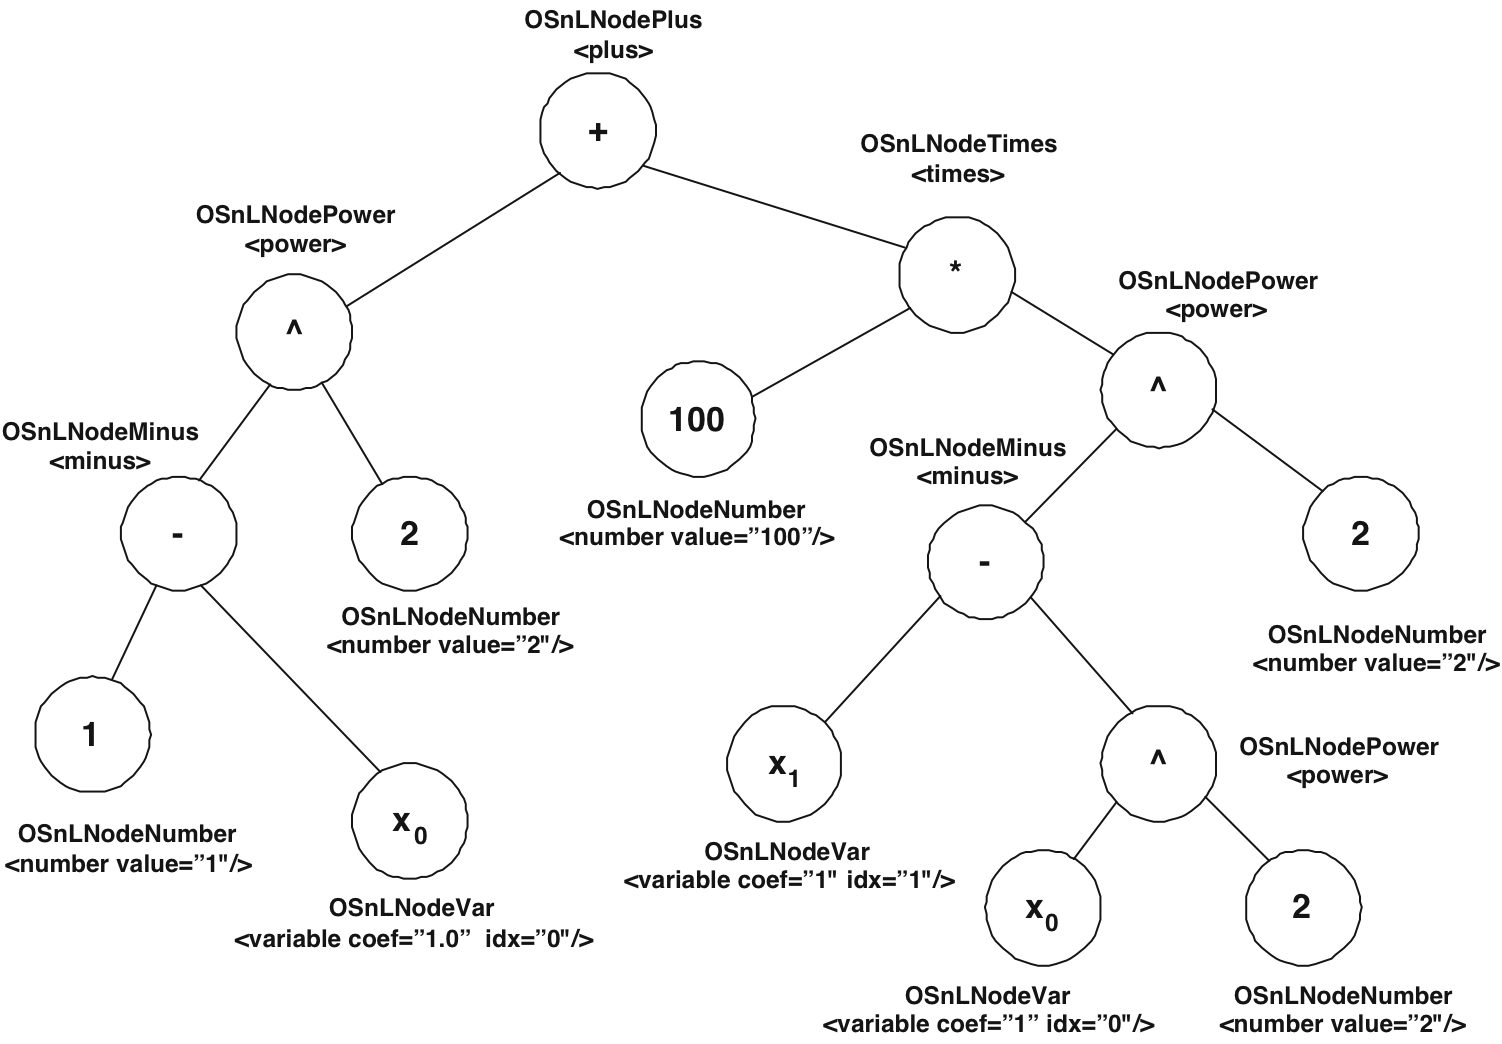
\includegraphics[%
  scale=0.38]{\figurepath/expressiontree.png}
\caption{Conceptual expression tree for the nonlinear part of the objective (\ref{eq:roobj}).} \label{figure:expressiontree}
\end{figure}


A base abstract class {\tt OSnLNode} is defined and  all of an OSiL file's
operator and operand elements used in defining a
nonlinear expression are extensions of the base element type {\tt OSnLNode}. There is an element type {\tt OSnLNodePlus}, for example, that
extends {\tt OSnLNode}; then in an OSiL instance
file, there are {\tt <plus>} elements that are of type {\tt
OSnLNodePlus}.   Each {\tt OSExpressionTree} object contains a pointer to an {\tt OSnLNode} object that is the root of the corresponding expression tree.  To every element that extends the {\tt OSnLNode} type in an OSiL instance file, there corresponds a class that derives from the {\tt OSnLNode} class in an {\tt OSInstance} data structure.  Thus we can construct an expression tree of homogenous nodes, and methods that operate on the expression tree to calculate function values, derivatives, postfix notation, and the like do not require switches or complicated logic.


\begin{figure}[ht]
\centering
   \small {\obeyspaces\let =\
\fbox{\tt\begin{tabular}{@{}l@{}}
   double OSnLNodePlus::calculateFunction(double *x)\{\\[\Sb]
      m\_dFunctionValue = \\[\Sb]
         m\_mChildren[0]->calculateFunction(x) +\\[\Sb]
         m\_mChildren[1]->calculateFunction(x);\\[\Sb]
      return m\_dFunctionValue;\\[\Sb]
   \} //calculateFunction\\[\Sb]
\end{tabular} }} \medskip
\caption{The function calculation method for the ``plus'' node class with polymorphism}
   \vspace{-8pt} \label{figure:calcfunction}
\end{figure}


    The {\tt OSInstance} class has a variety of {\tt calculate()} methods, based on two pure virtual functions in the {\tt OSInstance} class.  The first of these, {\tt calculateFunction()}, takes an array of {\tt double} values corresponding to decision variables, and evaluates the expression tree for those values.  Every class
that extends {\tt OSnLNode} must implement this method.  As an example, the {\tt calculateFunction} method for the {\tt OSnLNodePlus} class is shown in Figure \ref{figure:calcfunction}.  Because the OSiL instance file must be validated against its schema, and in the schema each {\tt <OSnLNodePlus>} element is specified to have exactly two child elements, this {\tt calculateFunction} method can assume that there are
exactly two children of the node that it is operating on.  The use of polymorphism and recursion makes adding new operator elements easy; it is simply a matter of adding a new class and implementing the {\tt
calculateFunction()} method for it.



Although in the OSnL schema, there are 200+ nonlinear operators, only the following {\tt  OSnLNode} classes are currently supported in our implementation.

\begin{itemize}
\item OSnLNodeVariable
\item OSnLNodeTimes
\item OSnLNodePlus
\item OSnLNodeSum
\item OSnLNodeMinus
\item OSnLNodeNegate
\item OSnLNodeDivide
\item OSnLNodePower
\item OSnLNodeProduct
\item OSnLNodeLn
\item OSnLNodeSqrt
\item OSnLNodeSquare
\item OSnLNodeSin
\item OSnLNodeCos
\item OSnLNodeExp
\item OSnLNodeif
\item OSnLNodeAbs
\item OSnLNodeMax
\item OSnLNodeMin
\item OSnLNodeE
\item OSnLNodePI
\item OSnLNodeAllDiff
\end{itemize}



\subsection{OSModelInterfaces}\label{section:osmodelinterfaces}

This part of the OS library is designed to help integrate the OS standards with other standards and modeling systems.

\subsubsection{Converting MPS Files}

The MPS standard is still a popular format for representing linear and integer programming problems.  In {\tt OSModelInterfaces,} there is a class {\tt OSmps2osil} that can be used to convert files in MPS format into the OSiL standard. It is used as follows.

\begin{verbatim}
OSmps2osil *mps2osil = NULL;
DefaultSolver *solver  = NULL;
solver = new CoinSolver();
solver->sSolverName = "cbc";
mps2osil = new OSmps2osil(  mpsFileName);
mps2osil->createOSInstance() ;
solver->osinstance = mps2osil->osinstance;
solver->solve();
\end{verbatim}

The {\tt OSmps2osil} class constructor takes a string which should be the file name of the instance in MPS format. The constructor then uses the CoinUtils library to read and parse the MPS file.  The class method {\tt createOSInstance} then builds  an in-memory {\tt osintance} object  that can be used by a solver.


\subsubsection{Converting AMPL nl Files}\label{section:nl2osil}

AMPL is a popular modeling language that saves  model instances in the AMPL nl format.  The {\tt OSModelInterfaces} library provides a class, {\tt OSnl2osil} for reading in an nl file and creating a corresponding in-memory osinstance object. It is used as follows.

\begin{verbatim}
OSnl2osil *nl2osil = NULL;
DefaultSolver *solver  = NULL;
solver = new LindoSolver();
nl2osil = new OSnl2osil( nlFileName);
nl2osil->createOSInstance() ;
solver->osinstance = nl2osil->osinstance;	
solver->solve();
\end{verbatim}


The {\tt OSnl2osil} class works much like the {\tt OSmps2osil} class. The {\tt OSnl2osil} class constructor takes a string which should be the file name of the instance in nl format. The constructor then uses the AMPL ASL library routines to read and parse the nl file. The class method {\tt createOSInstance} then builds  an in-memory {\tt osintance} object  that can be used by a solver.

In Section  \ref{section:amplclient}  we describe the {\tt amplClient} executable that acts a ``solver'' for AMPL. The {\tt amplClient} uses the {\tt OSnl2osil} class to convert the instance in nl format to OSiL format before calling a solver either locally or remotely.

\subsubsection{Using MATLAB}\label{section:usingmatlab}

Linear, integer, and quadratic problems can be formulated in MATLAB and then optimized either locally or over the network using the OS Library. The {\tt OSMatlab} class functions much like {\tt OSnl2osil} and {\tt OSmps2osil} and takes MATLAB arrays and creates and OSiL instance.  This class is part of the OS library. In order to use the OS library with MATLAB the user should do the following.  In order to use the {\tt OSMatlab} class it is necessary to  compile {\tt matlabSolver.cpp}  into  a MATLAB Executable file.  The {\tt matlabSolver.cpp} file is in the {\tt OSModelInterfaces} directory even though it is not part of the OS library. The following steps should be followed.

\begin{itemize}


\item[{\bf Step  1:}] In the project root run {\tt make install.}

\item[{\bf Step  2:}]   Either leave {\tt matlabSolver.cpp} in the  the {\tt OSModelInterfaces} or copy it to another desired directory.

\item[{\bf Step 3:}] Edit the MATLAB  {\bf mexopts.sh} (UNIX) or {\tt mexopts.bat}  so that the {\tt CXXFLAGS} option includes the header files in the {\tt cppad} directory and the {\tt include} directory in the project root. For example, it  should look like:
\begin{verbatim}
CXXFLAGS='-fno-common -no-cpp-precomp -fexceptions
    -I/Users/kmartin/Documents/files/code/cpp/OScpp/COIN-OSX/
    -I/Users/kmartin/Documents/files/code/cpp/OScpp/COIN-OSX/include'
\end{verbatim}

Next edit the {\tt CXXLIBS} flag so that the OS and supporting libraries are included. For example, it should look like:

\begin{verbatim}
CXXLIBS="$MLIBS -lstdc++
    -L/Users/kmartin/Documents/files/code/ipopt/macosx/Ipopt-3.2.2/lib
    -L/Users/kmartin/Documents/files/code/cpp/OScpp/COIN-OSX/lib
    -lOS  -lIpopt -lOsiCbc -lOsiClp -lCbc -lCgl -lOsi -lClp -lCoinUtils  -lm"
\end{verbatim}

For a UNIX system the {\tt mexopts.sh} file will usually be found in a directory with the release name in {\tt  $\sim$/.matlab}. For example,
{\tt $\sim$/.matlab/R14SP3}.


On a Windows system, the {\tt  mexopts.bat} file will usually be in a directory with the release name in {\tt C:$\backslash$Documents and Settings$\backslash$Username$\backslash$Application Data$\backslash$Mathworks$\backslash$MATLAB}


\item[{\bf Step 4:}]  Build the MATLAB executable file. Start MATLAB and in the MATLAB command window connect to the directory containing the file {\tt matlabSolver.cpp}.  Execute the command:

\begin{verbatim}
mex -v matlabSolver.cpp
\end{verbatim}

On a MAC OS X the resulting executable will be named {\tt matlabSolver.mexmac}. On the Windows system the file we named {\tt matlabSolver.mexw32}.

\item[{\bf Step 5:}]  Set the MATLAB path to include the directory with the {\tt matlabSolver} executable. Also, put  the $m-file$ {\tt callMatlabSolver.m} in a directory which is on a MATLAB path.  The  {\tt callMatlabSolver.m} m-file is in the OSModelInterfaces directory.

\end{itemize}


To use the {\tt matlabSolver} it is necessary to put the coefficients  from a linear, integer, or quadratic problem into MATLAB arrays.

\begin{alignat}{2}
& \mbox{Minimize} & \quad
10 x_{1} + 9 x_{2}\label{eq:parinobj}\\
& \mbox{Subject to} & \quad .7x_{1} + x_{2}  &\le 630  \label{eq:parinccon1}\\
& & .5x_{1} + (5/6) x_{2} &\le 600 \label{eq:parinccon2}\\
& &  x_{1} + (2/3) x_{2} &\le 708 \label{eq:parinccon3}\\
& & .1x_{1} + .25 x_{2} &\le 135 \label{eq:parinccon4}\\
& & x_{1}, x_{2} &\ge 0 \label{eq:parincnonneg}
\end{alignat}

The MATLAB representation of this problem in MATLAB arrays is
\begin{verbatim}
% the number of constraints
numCon = 4;
% the number of variables
numVar = 2;
% variable types
VarType='CC';
% constraint types
A = [.7  1; .5  5/6; 1   2/3  ; .1   .25];
BU = [630 600  708  135];
BL = [];
OBJ = [10  9];
VL = [-inf -inf];
VU = [];
ObjType = 1;
% leave Q empty if there are no quadratic terms
Q = [];
prob_name = 'ParInc Example'
password = 'chicagoesmuyFRIO';
%
%
%the solver
solverName = 'lindo';
%the remote service service address
%if left empty we solve locally
serviceAddress='http://gsbkip.chicagogsb.edu/os/OSSolverService.jws';
% now solve
callMatlabSolver( numVar, numCon, A, BL, BU, OBJ, VL, VU, ObjType, ...
    VarType, Q, prob_name, password, solverName, serviceAddress)
\end{verbatim}
This example m-file is in the {\tt data} directory and is file {\tt parincLinear.m}. Note that in addition to the problem formulation we can specify which solver to use through the {\tt solverName} variable.  If solution with a remote solver is desired this can be specified with the {\tt serviceAddress} variable.  If the {\tt serviceAddress} is left empty, i.e.
\begin{verbatim}
serviceAddress='';
\end{verbatim}
then a local solver is used. In this case  it is crucial that the appropriate solver is linked in with the {\tt matlabSolver} executable using the {\tt CXXLIBS} option.


The data directory  also contains the m-file  {\tt template.m} which contains extensive comments about how to formulate the problems in MATLAB.  A second example which is a quadratic problem is given in the Appendix. The appropriate m-file is {\tt markowitz.m}.



\subsection{OSParsers}

The OSParsers component of the OS library contains reentrant parsers that  read OSiL and OSrL strings and build, respectively, in-memory OSInstance and OSResult  objects.


The OSiL parser is invoked through an {\tt OSiLReader} object as illustrated below. Assume {\tt osil} is a string with the problem instance.
\begin{verbatim}
OSiLReader *osilreader = NULL;
OSInstance *osinstance = NULL;
osilreader = new OSiLReader();
osinstance = osilreader->readOSiL( &osil);
\end{verbatim}
The {\tt  readOSiL} method  has a single argument which is a pointer to a string. The {\tt  readOSiL} method then calls an underlying method {\tt yygetOSInstance} that parses the OSiL string. The major components of the OSiL schema are recognized by the parser.
\begin{verbatim}
<instanceHeader>
<variables>
<objectives>
<constraints>
<linearConstraintCoefficients>
<quadraticCoefficients>
<nonlinearExpressions>
\end{verbatim}
There are other components in the OSiL schema, but they are not yet implemented. In most large-scale applications the {\tt <variables>,} {\tt <objectives>}, {\tt <constraints>}, and {\tt }  will comprise the bulk of the instance memory.  Because of this, we have ``hard-coded'' the OSiL parser to read these specific elements very efficiently. The parsing of the {\tt <quadraticCoefficients>} and {\tt <nonlinearExpressions>} is done using code generated by {\tt flex} and {\tt bison}. In the {\tt OSParsers}  the file  {\tt paresosil.l} is used by {\tt flex} to generate {\tt parseosil.cpp} and the file {\tt parseosil.y} is used by {\tt bison} to generate {\tt parseosil.tab.cpp}.  In {\tt parseosil.l} we use the {\tt reentrant} option and in {\tt parseosil.y} we use the {\tt pure-parser} option to generate reentrant parsers. The {\tt parseosil.y} file  contains both our  ``hard-coded'' parser and the grammar rules for the  {\tt <quadraticCoefficients>} and {\tt <nonlinearExpressions>} sections.   We are currently using GNU Bison version 3.2 and {\tt flex} 2.5.33.

The typical OS user will have no need to edit either {\tt parseosil.l} or {\tt parseosil.y} and therefore will not have to worry about running either {\tt flex} or {\tt bison} to generate the parsers. The generated parser code from {\tt flex} and {\tt bison} is distributed with the project and works on all of the platforms listed in Table \ref{table:testedplatforms}.  If the user does edit either {\tt parseosil.l} or {\tt parseosil.y} then {\tt parseosil.cpp} and {\tt parseosil.tab.cpp} need to be regenerated with {\tt flex} and {\tt bison}. If these programs are present, in the OS directory  execute
\begin{verbatim}
make  run_parsers
\end{verbatim}

The files {\tt parseosrl.l} and {\tt parseosrl.y} are used by {\tt flex} and {\tt bison} to  generate the code {\tt parseosrl.cpp} and {\tt parseosrl.tab.cpp} for parsing strings in OSrL format. The comments made above about the OSiL parser apply to the OSrL parser. The OSrL parser, like the OSiL parser, is invoked using an {\tt OSrL} reading object. This is illustrated below ({\tt osrl} is a string in OSrL format).
\begin{verbatim}
OSrLReader *osrlreader = NULL;
osrlreader = new OSrLReader();
OSResult *osresult = NULL;
osresult = osrlreader->readOSrL( osrl);
\end{verbatim}

There is also a lexer {\tt parseosss.l} for tokenizing the command line for the OSSolverService executable described in Section \ref{section:ossolverservice}.

We hope to have a parser for OSoL  in a future version of the project.


\subsection{OSSolverInterfaces}\label{section:ossolverinterfaces}


The {\tt OSSolverInterfaces} library is designed to facilitate linking the OS library with various solver APIs. We first describe how to take a problem instance in OSiL format and connect to a solver that has a COIN-OR OSI interface.  See the OSI project \url{www.projects.coin-or.org/Osi}.   We then describe hooking to the COIN-OR nonlinear code {\tt Ipopt.} See \url{www.projects.coin-or.org/Ipopt}.  Finally we describe hooking to two commercial solvers KNITRO and LINDO.

The OS library has been tested with the following solvers using the Osi Interface.

\begin{itemize}
\item Cbc
\item Clp
\item Cplex
\item DyLP
\item Glpk
\item SYMPHONY
\item Vol
\end{itemize}

In the {\tt OSSolverInterfaces} library there is an abstract class {\tt DefaultSolver} that has the following key members:

\begin{verbatim}
std::string osil;
std::string osol;
std::string osrl;
OSInstance *osinstance;
OSResult  *osresult;
\end{verbatim}
and the pure virtual function
\begin{verbatim}
virtual void solve() = 0 ;	
\end{verbatim}
In order to use a solver through the COIN-OR {\tt Osi} interface it is necessary to an object in the {\tt CoinSolver} class which inherits from the {\tt DefaultSolver} class and implements the appropriate {\tt solve()} function.  We illustrate with the Clp solver.

\begin{verbatim}
DefaultSolver *solver  = NULL;
solver = new CoinSolver();
solver->m_sSolverName = "clp";
\end{verbatim}

Assume that the data file containing the problem has been read into the string {\tt osil} and the solver options are in the string {\tt osol}. Then the {\tt Clp} solver is invoked as follows.

\begin{verbatim}
solver->osil = osil;
solver->osol = osol;
solver->solve();
\end{verbatim}

Finally, get the solution in {\tt OSrL} format as follows

\begin{verbatim}
cout << solver->osrl << endl;
\end{verbatim}

Even though LINDO and KNITRO are commercial solvers and do not have a COIN-OR {\tt Osi} interface these solvers are used in exactly the same manner as a COIN-OR solver. For example, to invoke the LINDO solver we do the following.

\begin{verbatim}
solver = new LindoSolver();	
\end{verbatim}

Similarly for KNITRO and Ipopt. In the case of the KNITRO, the {\tt KnitroSolver} class inherits from both {\tt DefaultSolver} class and the KNITRO {\tt NlpProblemDef} class. See \url{http://www.ziena.com/docs/knitroman.pdf} for more information on the KNITRO solver C++ implementation and the {\tt NlpProblemDef} class. Similarly, for Ipopt the {\tt IpoptSolver} class inherits from both the  {\tt DefaultSolver} class and the Ipopt {\tt TNLP} class.  See \url{https://projects.coin-or.org/Ipopt/browser/stable/3.2/Ipopt/doc/documentation.pdf?format=raw} for more information on the Ipopt solver C++ implementation and the {\tt TNLP} calss.

In the examples above the problem instance was assumed to be read from a file into the string {\tt osil} and then into the class member {\tt solver->osil.} However, everything can be done entirely in memory. For example, it is possible to use the {\tt OSInstance} class to create an in-memory problem representation and give this representation directly to a solver class that inherits from {\tt DefaultSolver}. The class member to use is {\tt osinstance.} This is illustrated in the example given in Section \ref{subsection:exampleOSInstanceGeneration}.


\subsection{OSUtils}

The OSUtils component of the OS library contains utility codes. For example, the {\tt FileUtil} class contains useful methods for reading files into {\tt string} or {\tt char*} and writing files from {\tt string} and {\tt char*}.  The {\tt OSDataStructures} class holds other classes for things such as sparse vectors, sparse Jacobians, and sparse Hessians. The {\tt MathUtil} class contains a method for converting between sparse matrices in row and column major form.


\section{The  OSInstance API}\label{section:osinstanceAPI}

The OSInstance API can be used to:

\begin{itemize}

\item  get information about model parameters, or convert the {\tt OSExrpressionTree} into a prefix or postfix representation through a set of {\tt get} methods,

\item modify, or even create an instance from scratch, using a set of {\tt set} methods,

\item provide information to solvers that require function evaluations, Jacobian and Hessian sparsity patters,  function gradient evaluations, and Hessian evaluations.

\end{itemize}



\subsection{Get Methods}

The {\tt get()} methods are used by other classes to access data in an existing {\tt OSInstance} object or get an expression tree representation of an instance in postfix or prefix format.   Assume {\tt osinstance} is an object in the {\tt OSInstance} class created as illustrated in Figure \ref{figure:creatingosinstanceobject}. Then, for example,
\begin{verbatim}
osinstance->getVariableNumber();
\end{verbatim}
will return an integer which is the number of variables in the problem,
\begin{verbatim}
osintance->getVariableTypes();
\end{verbatim}
will return a {\tt char} pointer to the variable types ({\tt C} for continuous, {\tt B} for binary, and {\tt I} for general integer),
\begin{verbatim}
getVariableLowerBounds();
\end{verbatim}
will  return a {\tt double} pointer to the lower bound on each variable. There are similar {\tt get} methods for the constraints. There are numerous {\tt get} methods for the data in the {\tt <linearConstraintCoefficients>}  element, the {\tt <quadraticCoefficients>} element, and the {\tt <nonlinearExpressions>} element.

When an {\tt osinstance} object is created, it is stored as in expression tree in an {\tt OSExpressionTree} object. However, some solver APIs (e.g. LINDO) may take the data in a different format such as postfix and prefix. There are methods to return the data in either postfix or prefix format.

First define a {\tt vector} of pointers to {\tt OSnLNode} objects.
\begin{verbatim}
std::vector<OSnLNode*> postfixVec;
\end{verbatim}
then get the expression tree for the objective function (index = -1) as a postfix vector of nodes.
\begin{verbatim}
postfixVec = osinstance->getNonlinearExpressionTreeInPostfix( -1);
\end{verbatim}
If, for example, the {\tt osinstance} object was the in-memory representation of   the instance illustrated in  Section \ref{section:rosenbrockXML} then the code
\begin{verbatim}
for (i = 0 ; i < n; i++){
	cout << postfixVec[i]->snodeName << endl;	
}
\end{verbatim}
will produce
\begin{verbatim}
number
variable
minus
number
power
number
variable
variable
number
power
minus
number
power
times
plus
\end{verbatim}
The method, {\tt processNonlinearExpressions()} in the {\tt LindoSolver} class in the {\tt OSSolverInterfaces} library component illustrates using a postfix vector of {\tt OSnLNode} objects to build a Lindo model instance.


\subsection{Set Methods}

The {\tt set} methods can be used to build an in-memory {\tt OSInstance}
 object. A code example of how to do this is in Section \ref{subsection:exampleOSInstanceGeneration}.

\subsection{Calculate Methods}

The calculate methods are described in Section \ref{section:ad}.

\section{The OS Algorithmic Differentiation Implementation}\label{section:ad}

The OS library provides a set of {\tt calculate} methods for calculating  function values, gradients, and Hessians.     The {\tt calculate} methods are part of the {\tt OSInstance} class and are designed to work with solver APIs.



\subsection{Algorithmic Differentiation:  Brief Review}\label{section:adtheory}

First and second derivative calculations are made using {\it  algorithmic differentiation}.  Here we provide a brief review of algorithmic differentiation.  For an excellent reference on algorithmic differentiation see Griewank \cite{griewank2000}.  The OS package uses the COIN-OR package CppAD which  is also an excellent resource with extensive  documentation and information about algorithmic differentiation. See the documentation written by  Brad Bell \cite{bell2007}.    The development here is from the CppAD documentation.  Consider the function $f:X \rightarrow Y$ from $ \mathbb{R}^{n}$ to $ \mathbb{R}^{m}.$

Express the input vector as scalar function of $t$ by
\begin{eqnarray}
X(t) = x^{(0)} +  x^{(1)} t +  x^{(2)} t^{2}
\end{eqnarray}
where $ x^{(0)},$ $x^{(1)},$ and $x^{(2)}$ are vectors in $ \mathbb{R}^{n}.$ Then
\begin{eqnarray*}
X(0) &=& x^{(0)} \\
X^{\prime}(0) &=& x^{(1)} \\
X^{\prime \prime }(0) &=& 2 x^{(2)}
\end{eqnarray*}
In general the $x^{(k)}$ corresponds to the $k'th$ order Taylor coefficient, i.e.
\begin{eqnarray}
x^{(k)} = \frac{1}{k!}X^{(k)}(0), \quad k = 0, 1, 2  \label{eq:xTaylorCoeff}
\end{eqnarray}
Then $Y(t) = f(X(t))$ is a function from $ \mathbb{R}^{1}$ to $ \mathbb{R}^{m}$ and it is expressed in terms of its Taylor series expansion as
\begin{eqnarray}
Y(t)  = y^{(0)} +  y^{(1)} t +  y^{(2)} t^{2} + o(t^{3})
\end{eqnarray}
where
\begin{eqnarray}
y^{(k)} = \frac{1}{k!} Y^{(k)}(0), \quad k = 0, 1, 2  \label{eq:yTaylorCoeff}
\end{eqnarray}



It is shown by Bell (\url{http://www.coin-or.org/CppAD/}) that:
\begin{eqnarray}
y^{(0)} = f(x^{(0)}) \label{eq:forward0Result}
\end{eqnarray}
Let $e^{(i)}$ denote the $i'th$ unit vector.  If $x^{(1)} = e^{(i)}$ then $y^{(1)}$ is equal to the $i'th$ column of the Jacobian matrix of $f(x)$ evaluated at $x^{(0)}.$ That is
\begin{eqnarray}
y^{(1)} = \D{f}{x_{i}}(x^{(0)}).  \label{eq:forward1Result}
\end{eqnarray}

If $x^{(1)} = e^{(i)}$ and $x^{(2)} = 0$ then for function $f_{k}(x),$
\begin{eqnarray}
y^{(2)}_{k} =  \frac{1}{2} \DD{f_{k}(x^{(0)})}{x_{i}}{x_{i}}  \label{eq:forward2Resulta}
\end{eqnarray}

If $x^{(1)} = e^{(i)} + e^{(j)}$ and $x^{(2)} = 0$ then for function $f_{k}(x),$
\begin{eqnarray}
y^{(2)}_{k} =  \frac{1}{2} \left( \DD{f_{k}(x^{(0)})}{x_{i}}{x_{i}}  +   \DD{f_{k}(x^{(0)})}{x_{i}}{x_{j}} +  \DD{f_{k}(x^{(0)})}{x_{j}}{x_{i}} +  \DD{f_{k}(x^{(0)})}{x_{j}}{x_{j}}  \right) \label{eq:forward2Resultb}
\end{eqnarray}
or, expressed in terms of the mixed partials,
\begin{eqnarray}
  \DD{f_{k}(x^{(0)})}{x_{i}}{x_{j}}  = y_{k}^{(2)}  -  \frac{1}{2} \left( \DD{f_{k}(x^{(0)})}{x_{i}}{x_{i}}  +  \DD{f_{k}(x^{(0)})}{x_{j}}{x_{j}}  \right) \label{eq:forward2Resultc}
\end{eqnarray}





\subsection{Using OSInstance Methods: Low Level Calls}

  The code snippets used in this section  are from the example code {\tt algorithmicDiffTest.cpp} in the {\tt algorithmicDiffTest} folder in the {\tt examples} folder.  The  code is based on the following example.

\begin{alignat}{2}
& \mbox{Minimize} & \quad  x_{0}^{2} + 9x_{1} \label{eq:adobj}\\
& \mbox{s.t.} & 33 - 105 + 1.37 x_{1} + 2x_{3} + 5 x_{1} &\le 10  \label{eq:adeq0}\\
& & \ln(x_{0} x_{3}) + 7x_{2} &\ge 10 \label{eq:adeq1} \\
& & x_{0}, x_{1}, x_{2}, x_{3} &\ge 0 \label{eq:adeq2}
\end{alignat}

The OSiL representation of the instance  (\ref{eq:adobj})-(\ref{eq:adeq2}) is given in Appendix \ref{section:adexample}.  This example is designed to illustrate several features of OSiL. Note that in equation (\ref{eq:adeq0}) the constant 33 appears in the {\tt <con>} element corresponding to this constraint and the constant 105 appears as a {\tt <number>} OSnL node in the {\tt <nonlinearExpressions>} section.  There are no nonlinear terms in the instance that involve variable $x_{1}.$  The $5 x_{1}$ term in equation (\ref{eq:adeq0}) is expressed in the {\tt <linearConstraintCoefficients>} section.  However,  the $1.37 x_{1}$ term in equation (\ref{eq:adeq0}) is expressed in the {\tt <nonlinearExpressions>} section.  Hence, in the OSInstance API, variable $x_{1}$ is treated as a nonlinear variable for purposes of algorithmic differentiation. Variable $x_{2}$ never appears in the  {\tt <nonlinearExpressions>} section and is therefore treated as a linear variable and not used  in any algorithmic differentiation calculations.

Ignoring the nonnegativity constraints, instance (\ref{eq:adobj})-(\ref{eq:adeq2})  defines the following function $f:X \rightarrow Y$ from $ \mathbb{R}^{4}$ to $ \mathbb{R}^{3}.$

\begin{eqnarray}
f(x) =
\left[
\begin{array}{r}
f_{1}(x) \\
f_{2}(x) \\
f_{3}(x)
\end{array}
\right]
=
\left[
\begin{array}{r}
x_{0}^{2} + 9x_{1}  \\
33 - 105 + 1.37 x_{1} + 2x_{3} + 5 x_{1} \\
\ln(x_{0} x_{3}) + 7x_{2}
\end{array}
\right] \label{eq:definef}
\end{eqnarray}


The OSiL representation for the instance  in  (\ref{eq:adobj})-(\ref{eq:adeq2})  is read into an in-memory OSInstance object as follows (we assume that {\tt osil} is a {\tt string} with the OSiL instance)
\begin{verbatim}
osilreader = new OSiLReader();
osinstance = osilreader->readOSiL( &osil);
\end{verbatim}
There is a method in the {\tt OSInstance} class, {\tt initForAlgDiff()} that is used to initialize the nonlinear data structures.  A call to this method
\begin{verbatim}
osinstance->initForAlgDiff( );
\end{verbatim}
will generate a map of the indices of the nonlinear variables. This is critical because the algorithmic differentiation only operates on variables that appear in the {\tt <nonlinearExpressions>} section.  An example of this map follows.
\begin{verbatim}
std::map<int, int> varIndexMap;
std::map<int, int>::iterator posVarIndexMap;
varIndexMap = osinstance->getAllNonlinearVariablesIndexMap( );
for(posVarIndexMap = varIndexMap.begin(); posVarIndexMap
	!= varIndexMap.end(); ++posVarIndexMap){
	std::cout <<  "Variable Index = "   << posVarIndexMap->first  << std::endl ;
}
\end{verbatim}
The variable indices listed are 0, 1, and 3. Variable 2 does not appear in the {\tt <nonlinearExpressions>} section and is not included in {\tt varIndexMap}.

Once the nonlinear structures are initialized it is possible to take derivatives using algorithmic differentiation.   Algorithmic differentiation is done using either a forward or reverse sweep through an expression tree (or operation sequence) representation of $f$.  The two key algorithmic differentiation {\tt public} methods in the {\tt OSInstance} class are {\tt forwardAD} and {\tt reverseAD}.   These are actually  generic ``wrappers'' around the corresponding CppAD methods with the same signature.  This keeps the OS API  public methods independent of any underlying algorithmic differentiation package.

The {\tt forwardAD} signature is
\begin{verbatim}
std::vector<double> forwardAD(int k, std::vector<double> vdX);
\end{verbatim}
where $k$ is the highest order Taylor coefficient of $f$ to be returned,  $\tt vdX$ is vector of doubles in $ \mathbb{R}^{n},$ and the function return is a vector of doubles in $ \mathbb{R}^{m}.$  Thus, $k$ corresponds to the $k$ in Equations  (\ref{eq:xTaylorCoeff}) and (\ref{eq:yTaylorCoeff}),  where {\tt vdX} corresponds to the $x^{(k)}$ in Equation (\ref{eq:xTaylorCoeff}) and the $y^{(k)}$ in Equation (\ref{eq:yTaylorCoeff}) is the vector in range space returned by the call to {\tt  forwardAD}.    For example, by  Equation (\ref{eq:forward0Result}) the following call will evaluate each component function defined in (\ref{eq:definef}).
\begin{verbatim}
funVals = osinstance->forwardAD(0, x0);
\end{verbatim}
Since there are three components in the vector defined by  (\ref{eq:definef}), the return value  {\tt funVals} will have three components. For an input vector,
\begin{verbatim}
x0[0] = 1; // the value for variable x0
x0[1] = 5; // the value for variable x1
x0[2] = 5; // the value for variable x3
\end{verbatim}
the values returned by {\tt osinstance->forwardAD(0, x0)}  are 1, -63.15, and 1.6094, respectively.
The Jacobian of the example in (\ref{eq:definef}) is

\begin{eqnarray}
J =
\left[
\begin{array}{rrrr}
2x_{0} &9.00&0.00&0.00   \\
0.00&6.37&0.00&2.00 \\
1/x_{0}&0.00&7.00&1/x_{3}
\end{array}
\right] \label{eq:jac}
\end{eqnarray}
when $x_{0} = 1,$ $x_{1} = 5,$ $x_{2} = 10,$ and $x_{3} = 5$ the Jacobian is
\begin{eqnarray}
J =
\left[
\begin{array}{rrrr}
2.00 &9.00&0.00&0.00   \\
0.00&6.37&0.00&2.00 \\
1.00&0.00&7.00&0.20
\end{array}
\right] \label{eq:jac2}
\end{eqnarray}
A forward sweep with $k = 1$ will calculate the Jacobian column-wise.  See
(\ref{eq:forward1Result}).  The following code will return column 4 of the Jacobian (\ref{eq:jac2}) which corresponds to nonlinear variable $x_{3}.$
\begin{verbatim}
x1[0] = 0;
x1[1] = 0;
x1[2] = 1;
osinstance->forwardAD(1, x1);
\end{verbatim}

Now calculate second derivatives.  To illustrate we use the results in (\ref{eq:forward2Resulta})-(\ref{eq:forward2Resultc}) and calculate
\begin{eqnarray*}
\DD{f_{k}(x^{(0)})}{x_{0}}{x_{3}} \quad k = 1, 2, 3.
\end{eqnarray*}
Variables $x_{0}$ and $x_{3}$ are the first and third nonlinear variables so by  (\ref{eq:forward2Resultb}) the $x^{(1)}$ should be the sum of the $e^{(1)}$ and $e^{3}$ unit vectors and used in first-order forward sweep calculation.
\begin{verbatim}
x1[0] = 1;
x1[1] = 0;
x1[2] = 1;
osinstance->forwardAD(1, x1);
\end{verbatim}
Next set $x^{(2)} = 0$ and do a second-order forward sweep.
\begin{verbatim}
std::vector<double> x2( n);
x2[0] = 0;
x2[1] = 0;
x2[2] = 0;
osinstance->forwardAD(2, x2);
\end{verbatim}
This call returns the vector of  values
\begin{eqnarray*}
y_{1}^{(2)}  = 1, \quad y_{2}^{(2)}  = 0, \quad y_{3}^{(2)} = -.52
\end{eqnarray*}
By inspection,
\begin{eqnarray*}
\DD{f_{1}(x^{(0)})}{x_{0}}{x_{0}} &=& 2 \\
\DD{f_{2}(x^{(0)})}{x_{0}}{x_{0}} &=&  0\\
\DD{f_{3}(x^{(0)})}{x_{0}}{x_{0}} &=& -1 \\
\DD{f_{1}(x^{(0)})}{x_{3}}{x_{3}} &=& 0 \\
\DD{f_{2}(x^{(0)})}{x_{3}}{x_{3}} &=& 0\\
\DD{f_{3}(x^{(0)})}{x_{3}}{x_{3}} &=& -.04
\end{eqnarray*}
Then by (\ref{eq:forward2Resultc}),
\begin{eqnarray*}
\DD{f_{1}(x^{(0)})}{x_{0}}{x_{3}} &=&  y_{1}^{(2)}  -  \frac{1}{2} \left( \DD{f_{1}(x^{(0)})}{x_{0}}{x_{0}}  +  \DD{f_{k}(x^{(0)})}{x_{3}}{x_{3}}  \right) =   1 -  \frac{1}{2}(2 +  0) = 0 \\
\DD{f_{2}(x^{(0)})}{x_{0}}{x_{3}} &=&   y_{2}^{(2)}  -  \frac{1}{2} \left( \DD{f_{2}(x^{(0)})}{x_{0}}{x_{0}}  +  \DD{f_{k}(x^{(0)})}{x_{3}}{x_{3}}  \right)  = 0 -  \frac{1}{2}(0 +  0) = 0 \\
\DD{f_{3}(x^{(0)})}{x_{0}}{x_{3}} &=&  y_{3}^{(2)}  -  \frac{1}{2} \left( \DD{f_{3}(x^{(0)})}{x_{0}}{x_{0}}  +  \DD{f_{k}(x^{(0)})}{x_{3}}{x_{3}}  \right) = -52 -  \frac{1}{2}(-1 - .04) = 0
\end{eqnarray*}
Making all of the first and second derivative calculations using forward sweeps is most effective when the number of rows exceeds the number of variables.


The {\tt reverseAD} signature is
\begin{verbatim}
std::vector<double> reverseAD(int k, std::vector<double> vdlambda);
\end{verbatim}
where {\tt vdlambda} is a vector of Lagrange multipliers.  This method returns a vector in the range space. If a reverse sweep of order $k$ is called, a forward sweep of order at $k -1$ must have been made prior to the call.

\subsubsection{First Derivative Reverse Sweep Calculations}

In order to calculate first derivatives execute the following sequence of calls.
\begin{verbatim}
x0[0] = 1;
x0[1] = 5;
x0[2] = 5;
std::vector<double> vlambda(3);
vlambda[0] = 0;
vlambda[1] = 0;
vlambda[2] = 1;
osinstance->forwardAD(0, x0);
osinstance->reverseAD(1, vlambda);
\end{verbatim}
Since the {\tt vlambda} only includes the third function $f_{1}(x)$ the sequence of calls will produce the third row of the Jacobian, i.e.
$$
\D{f_{3}(x^{(0)})}{x_{0}}  = 1,  \quad \D{f_{3}(x^{(0)})}{x_{1}}  = 0, \quad  \D{f_{3}(x^{(0)})}{x_{3}}  = .2
$$

\subsubsection{Second Derivative Reverse Sweep Calculations}

In order to calculate second derivatives using {\tt reverseAD} forward sweeps of order 0 and 1 must be finished.  The call to {\tt reverseAD(2, vlambda)} will return a vector of dimension $2n$ where $n$ is the number of variables.  If the zero-order forward sweep is {\tt forward(0,x0)} and the first-order forward sweep is {\tt forwardAD(1, x1)} where $x1 = e^{(i)},$ then the return vector {\tt z = reverseAD(2,  vlambda)} is
\begin{eqnarray}
z[2j - 2]  = \D{L (x^{(0)}, \lambda^{(0)})}{x_{j}}, \quad j = 1, \ldots, n
\end{eqnarray}
\begin{eqnarray}
z[2j - 1]  = \DD{L(x^{(0)}, \lambda^{(0)})}{x_{i}}{x_{j}}, \quad j = 1, \ldots, n
\end{eqnarray}
where
\begin{eqnarray}
L (x, \lambda) = \sum_{k = 1}^{m} \lambda_{k} f_{k}(x)
\end{eqnarray}



For example, the  following calls will calculate the third row (column) of the Hessian of the Lagrangian.
\begin{verbatim}
x0[0] = 1;
x0[1] = 5; 	
x0[2] = 5;
osinstance->forwardAD(0, x0);	
x1[0] = 0;
x1[1] = 0;
x1[2] = 1;
osinstance->forwardAD(1, x1);
vlambda[0] = 1;
vlambda[1] = 2;
vlambda[2] = 1;
osinstance->reverseAD(2, vlambda);
\end{verbatim}
This returns
\begin{eqnarray*}
\D{L (x^{(0)}, \lambda^{(0)})}{x_{1}} = 3, \quad  \D{L (x^{(0)}, \lambda^{(0)})}{x_{2}} = 12.74, \quad  \D{L (x^{(0)}, \lambda^{(0)})}{x_{3}} = 4.2
\end{eqnarray*}
\begin{eqnarray*}
\DD{L(x^{(0)}, \lambda^{(0)})}{x_{3}}{x_{0}} =0, \quad  \DD{L(x^{(0)}, \lambda^{(0)})}{x_{3}}{x_{1}} = 0, \quad   \DD{L(x^{(0)}, \lambda^{(0)})}{x_{3}}{x_{3}} =  -.04
\end{eqnarray*}

The reason that
$$
\D{L (x^{(0)}, \lambda^{(0)})}{x_{2}} = 2 \times 6.37 = 12.74
$$
and not
$$
\D{L (x^{(0)}, \lambda^{(0)})}{x_{2}} = 1 \times  9 + 2 \times 6.37 = 12.74  = 21.74
$$
is that the $9x_{1}$ term in the objective is captured in the {\tt <coef>} element in the {\tt <objectives>} section and therefore does not appear as a nonlinear term in {\tt  <nonlinearExpressions>}. Again, {\tt forwardAD} and {\tt reverseAD} only operate on variables and terms in either the {\tt <quadraticCoefficients>} or {\tt <nonlinearExpressions>} sections.

\subsection{Using OSInstance Methods: High Level Calls}

The methods {\tt forwardAD} and {\tt reverseAD} are low level calls and are not designed to work directly with solver APIs. The {\tt OSInstance} API has other methods that most users will want to invoke when linking with solver APIs.  We describe these now.


\subsubsection{Sparsity Methods}

Many  solvers such as Ipopt (\url{projects.coin-or.org/Ipopt}) or Knitro (\url{www.ziena.com}) require the sparsity pattern of the Jacobian of the constraint matrix and the Hessian of the Lagrangian function. The following code illustrates how to get the sparsity pattern of the constraint Jacobian matrix
\begin{verbatimtab}[4]
SparseJacobianMatrix *sparseJac;
sparseJac = osinstance->getJacobianSparsityPattern();
for(idx = 0; idx < sparseJac->startSize; idx++){
	std::cout << "number constant terms in constraint "   <<  idx << " is "
	<< *(sparseJac->conVals + idx)  << std::endl;
	for(k = *(sparseJac->starts + idx); k < *(sparseJac->starts + idx + 1); k++){
		std::cout << "row idx = " << idx <<  "
		col idx = "<< *(sparseJac->indexes + k) << std::endl;
	}
}
\end{verbatimtab}
For the example problem this will produce
\begin{verbatim}
JACOBIAN SPARSITY PATTERN
number constant terms in constraint 0 is 0
row idx = 0  col idx = 1
row idx = 0  col idx = 3
number constant terms in constraint 1 is 1
row idx = 1  col idx = 2
row idx = 1  col idx = 0
row idx = 1  col idx = 3
\end{verbatim}
The {\tt SparseJacobianMatrix} object has a data member {\tt starts} which is the index of the start of each constraint row. The {\tt int} data member {\tt indexes} is the variable index of a potential nonzero derivative. There is also a {\tt double} data member  {\tt values} that will the value of the partial derivative of the corresponding index at each iteration. Finally, there is an {\tt int} data member {\tt conVals} that is the number of constant terms in each gradient. A constant term is a partial derivative that cannot change at an iteration.  A variable is considered a constant variable if it appears in the {\tt <linearConstraintCoefficients>} section  but not in the {\tt nonlinearExpressions}.  For a row indexed by {\tt idx} the variable indices are in the  {\tt indexes} array between the elements {\tt sparseJac->starts + idx} and {\tt sparseJac->starts + idx + 1.}   The first  {\tt sparseJac->conVals + idx} variables listed are indices of constant variables. In this example, when {\tt idx} is 1, there is one constant variable and it is variable $x_{2}.$  The constant variables never appear in the AD evaluation.

The following code illustrates how to get the sparsity pattern of the Hessian of the Lagrangian.
\begin{verbatim}
SparseHessianMatrix *sparseHessian;
sparseHessian = osinstance->getLagrangianHessianSparsityPattern( );
for(idx = 0; idx < sparseHessian->hessDimension; idx++){
	std::cout <<  "Row Index = " << *(sparseHessian->hessRowIdx + idx) ;
	std::cout <<  "  Column Index = " << *(sparseHessian->hessColIdx + idx);
}
\end{verbatim}
The {\tt SparseHessianMatrix} class has the {\tt int} data members {\tt hessRowIdx} and {\tt hessColIdx} for indexing  potential nonzero elements in the Hessian matrix. The {\tt double} data member {\tt hessValues} holds the value of the respective second derivative at each iteration.  If {\tt numVars} is the number of nonlinear variables, each array in {\tt sparseHessian} is of size
$$
numVars*(numVars + 1)/2;
$$
All mixed partials of nonlinear terms are considered to be potential nonzeros.  Hopefully, a future implementation of the OS library will be more robust in preserving sparsity.


\subsubsection{Function Evaluation Methods}

There are several overloaded methods for calculating objective and constraint values.  The method
\begin{verbatim}
double *calculateAllConstraintFunctionValues(double* x, bool new_x)
\end{verbatim}
will return a {\tt double} pointer to an array of constraint function values evaluated at {\tt x.}  If the value of {\tt x} has not changed since the last function call, then {\tt new\_x} should be set to {\tt false} and the most recent function values are returned.  When using this method, with this signature,  all function values are calculated in {\tt double} using an {\tt OSExpressionTree} object.

A second signature for the {\tt calculateAllConstraintFunctionValues} is
\begin{verbatim}
double *calculateAllConstraintFunctionValues(double* x, double *objLambda,
    double *conLambda, bool new_x, int highestOrder)
\end{verbatim}
In this  signature, {\tt x} is a pointer to the current primal values, {\tt objLambda} is a vector of dual multipliers, {\tt conLambda} is a vector of dual multipliers on the constraints,  {\tt new\_x} is true if any components of {\tt x} have changed since the last evaluation, and {\tt highestOrder} is the highest order of derivative to be calculated at this iteration. The following code snippet illustrates defining a set of variable values for the example we are using and then the function call.
\begin{verbatim}
double* x = new double[4]; //primal variables
double* z = new double[2]; //Lagrange multipliers on constraints
double* w = new double[1]; //Lagrange multiplier on objective
x[ 0] = 1;    // primal variable 0
x[ 1] = 5;    // primal variable 1
x[ 2] = 10;   // primal variable 2
x[ 3] = 5;    // primal variable 3
z[ 0] = 2;    // Lagrange multiplier on constraint 0
z[ 1] = 1;    // Lagrange multiplier on constraint 1
w[ 0] = 1;    // Lagrange multiplier on the objective function
calculateAllConstraintFunctionValues(x, w, z,  true, 0);
\end{verbatim}
When making all high level calls for function, gradient, and Hessian evaluations we pass all the primal variables in the {\tt x} argument, not just the nonlinear variables. Underneath the call, the nonlinear variables are identified and used in AD function calls.

The use of the parameters  {\tt new\_x} and {\tt highestOrder}  is important and requires further explanation.    The parameter  {\tt highestOrder}  is an integer variable that will take on the value 0, 1, or 2 (actually higher values if we want third derivatives etc.).  The value of this variable is the highest order derivative that is required of the current iterate. For example, if  a callback requires a function evaluation and {\bf highestOrder = 0} then only the function is evaluated at the current iterate.  However,  if {\tt highsetOrder = 2} then the function call
\begin{verbatim}
calculateAllConstraintFunctionValues(x, w, z, true, 2)
\end{verbatim}
will trigger  first and second derivative evaluations in addition to the function evaluations.

In the {\tt OSInstance} class code,  every time a forward ({\tt forwardAD}) or reverse sweep ({\tt reverseAD}) is executed a private  member, {\tt m\_iHighestOrderEvaluated}  is  set to the order of the sweep. For example, {\tt forwardAD(1, x)} will result in {\tt  m\_iHighestOrderEvaluated = 1}.  Just knowing the value  of  {\tt new\_x} alone is not sufficient. It is also necessary  to know {\tt highestOrder} and compare it with {\tt m\_iHighestOrderEvaluated.}  For example, if  {\tt new\_x}  is  false,  but {\tt m\_iHighestOrderEvaluated = 0},  and   the callback requires a Hessian calculation, then it is necessary to calculate the first and second derivatives at the current iterate.

There are {\it  exactly two} conditions that  require a new function or derivative evaluation.   A new evaluation is required if and only if

\begin{itemize}
\item[1.]   The value of {\tt new\_x} is  true

\begin{center}
 --OR--
\end{center}


\item[2.] For the callback function the value of the input parameter {\tt highestOrder} is strictly greater than the current value  of    {\tt m\_iHhighestOrderEvaluated.}
\end{itemize}

For an efficient implementation of AD it is important to be able to get the Lagrange multipliers and highest order derivative that is required from inside {\it any} callback -- not just the Hessian evaluation callback. For example, in {\tt Ipopt,} if  {\tt eval\_g}  or {\tt eval\_f} are called, and  for the current iterate, {\tt eval\_jac} and {\tt eval\_hess} are also going to be called, then  a more efficient AD implementation is possible if the Lagrange multipliers are available for {\tt eval\_g} and {\tt eval\_f}.

Currently, whenever {\tt new\_x = true} in the underlying AD implementation we do not retape the function. This is because we currently throw an exception if there are any logical operators involved in the AD calculations. This may change in a future implementation.


There are also similar methods for objective function evaluations.  There is also a method
\begin{verbatim}
double calculateFunctionValue(int idx, double* x, bool new_x);
\end{verbatim}
that will return the value of any constraint or objective function indexed by {\tt idx}. This method works strictly with {\tt double} data using an {\tt OSExpressionTree} object.

There is also a public variable, {\tt bUseExpTreeForFunEval} that, if set to {\tt true}, will cause the method
\begin{verbatim}
calculateAllConstraintFunctionValues(x, objLambda,  conLambda, true, highestOrder)
\end{verbatim}
to also use the OS expression tree for function evaluations when {\tt highestOrder = 0} rather than use the operator overloading in the CppAD tape.

\subsubsection{Gradient Evaluation Methods}

One {\tt OSInstance} method for gradient calculations is
\begin{verbatim}
SparseJacobianMatrix *calculateAllConstraintFunctionGradients(double* x, double *objLambda,
     double *conLambda, bool new_x, int highestOrder)
\end{verbatim}
If a call has been placed to {\tt calculateAllConstraintFunctionValues} with {\tt highestOrder = 0}, then the appropriate call to get gradient evaluations is
\begin{verbatim}
calculateAllConstraintFunctionGradients( x, NULL, NULL,  false, 1);
\end{verbatim}
Note that in this function call {\tt new\_x = false}. This prevents a call to {\tt forwardAD()} with order 0 to get the function values.


If, at the current iterate, the Hessian of the Lagrangian function is also desired then an appropriate call is
\begin{verbatim}
calculateAllConstraintFunctionGradients(x, objLambda, conLambda, false, 2);
\end{verbatim}
In this case, if there was a prior call
\begin{verbatim}
calculateAllConstraintFunctionValues(x, w, z,  true, 0);
\end{verbatim}
then only first and second derivatives are calculated, not function values.

When calculating the gradients, if the number of nonlinear variables exceeds or is equal  to the number of rows,  a {\tt forwardAD(0, x)} sweep is used to get the function values,  and   a {\tt reverseAD(1, $e^{k}$)}  sweep for each unit vector  $e^{k}$ in the row space  is used to get the vector of first order partials for each row in the constraint Jacobian.  If the number of nonlinear variables is less then the number of rows then a {\tt forwardAD(0, x)} sweep  is used to get the function values and a {\tt forwardAD(1,  $e^{i}$)}  sweep for each unit vector  $e^{i}$ in the column space is used to get the vector of first order partials for each column in the constraint Jacobian.

Two other gradient methods are
\begin{verbatim}
SparseVector *calculateConstraintFunctionGradient(double* x,
    double *objLambda, double *conLambda,  int idx, bool new_x, int highestOrder);
\end{verbatim}
and
\begin{verbatim}
SparseVector *calculateConstraintFunctionGradient(double* x, int idx,
    bool new_x );
\end{verbatim}

Similar methods are available for the objective function, however the objective function gradient methods treat the gradient of each objective function as a dense vector.


\subsubsection{Hessian Evaluation Methods}

There are two methods for Hessian calculations.  The first method has the signature
\begin{verbatim}
SparseHessianMatrix *calculateLagrangianHessian( double* x,
    double *objLambda, double *conLambda, bool new_x, int highestOrder);
\end{verbatim}
so if either function or first derivatives have been calculated an appropriate call is
\begin{verbatim}
calculateLagrangianHessian( x, w, z, false, 2);
\end{verbatim}
If the Hessian of a single row or objective function is desired the following method is available
\begin{verbatim}
SparseHessianMatrix *calculateHessian( double* x, int idx, bool new_x);
\end{verbatim}

\section{The OSSolverService}\label{section:ossolverservice}

The {\tt OSSolverService} is a command line executable designed to pass problem instances in either  OSiL, AMPL nl, or MPS format  to solvers and get the optimization result back to be displayed either to standard output or a specified browser.  The {\tt OSSovlerService} can be used to invoke a solver locally or on a remote server. It can work either synchronously or asynchronously.

\subsection{OSSolverService Input Parameters}

At present, the {\tt OSSolverService} takes the following parameters. The order of the parameters is irrelevant.  Not all the parameters are required. However, if the {\tt solve} or {\tt send} service methods are invoked a problem instance location must be specified.

\begin{itemize}

\item[] {\bf -osil xxx.osil}  this is the name of the file that contains the optimization instance in OSiL format. It is assumed that this file is available in a directory on the machine that is running {\tt OSSolverService}. If this option is not specified then the instance location must be specified in the OSoL solver options file.

\item[] {\bf -osol xxx.osol}  this is the name of the file that contains the solver options. It is assumed that this file is available in a directory on the machine that is running {\tt OSSolverService}. It is not necessary to specify this option.

\item[] {\bf -osrl xxx.osrl}  this is the name of the file that contains the solver solution. A valid file path must be given on the machine that is running {\tt OSSolverService}. It is not necessary to specify this option.

\item[] {\bf -serviceLocation url}  is the URL of the solver service. This is not required, and if not specified it is assumed that the problem is solved locally.

\item[] {\bf -serviceMethod  methodName}  this is  the method on the solver service to be invoked. The options are {\tt solve}, {\tt send}, {\tt kill}, {\tt knock}, {\tt getJobID}, and {\tt retrieve}. The use of these options is illustrated in the examples below. This option is not required, and the default value is {\tt solve.}

\item[] {\bf -mps  xxx.mps}  this is the name of the mps file if the problem instance is in mps format. It is assumed that this file is available in a directory on the machine that is running {\tt OSSolverService}. The default file format is OSiL so this option is not required.

\item[] {\bf -nl  xxx.nl}  this is the name of the AMPL nl file if the problem instance is in AMPL nl  format. It is assumed that this file is available in a directory on the machine that is running {\tt OSSolverService}. The default file format is OSiL so this option is not required.

\item[] {\bf -solver  solverName}  Possible values for default OS installation are {\tt clp} (COIN-OR Clp), {\tt cbc} (COIN-OR Cbc), {\tt dylp} (COIN-OR DyLP), and {\tt symphony} (COIN-OR SYMPHONY). Other solvers supported (if the necessary libraries are present) are {\tt cplex} (Cplex through COIN-OR Osi), {\tt glpk} (glpk through COIN-OR Osi), {\tt ipopt} (COIN-OR Ipopt),  {\tt knitro} (Knitro), and {\tt lindo} {\tt LINDO}. If no value is specified for this parameter, then {\tt cbc} is the default value of this parameter if the the {\tt solve} or {\tt send} service methods are used.


\item[] {\bf -browser  browserName} this paramater is a path to the browser on the local machine. If this optional parameter is specified then the solver result in OSrL format is transformed using XSLT into HTML and displayed in the browser.

\item[] {\bf -config pathToConfigureFile} this parameter specifies a path on the local machine to a text file containing values for the input parameters. This is convenient for the user not wishing to constantly retype parameter values.

\end{itemize}



The input parameters to the {\tt OSSolverService} may be given entirely in the command line or in a configuration file.  We first illustrate giving all the  parameters in the command line. The following command will invoke the {\tt Clp} solver on the local machine to solve the problem instance {\tt parincLinear.osil}.  When invoking the commands below involving {\tt OSSolverservice} we assume that 1) the user is connected to the directory where the {\tt OSSolverService} executable is located, and 2) that {\tt ../data/osilFiles} is a valid path to {\tt COIN-OS/data/osilFiles}.  If the OS project was built successfully, then there is a copy of  {\tt OSSolverService} in {\tt COIN-OS/OS/src}. The user may wish to execute {\tt OSSolverService} from this {\tt src} directory so that all that follows is correct in terms of path definitions.


\begin{verbatim}
./OSSolverService -solver clp -osil ../data/osilFiles/parincLinear.osil
\end{verbatim}

Alternatively, these parameters can be put into a configuration file. Assume that the configuration file of interest is {\tt testlocalclp.config}. It would contain the two lines of information
\begin{verbatim}
-osil ../data/osilFiles/parincLinear.osil
-solver clp
\end{verbatim}
Then the command line is
\begin{verbatim}
./OSSolverService -config ../data/configFiles/testlocalclp.config
\end{verbatim}


{\bf Some Rules:}

\begin{itemize}
\item[1.]  When using the {\tt send()} or  {\tt solve()} methods a problem instance file location {\it must} be specified either at  the command line, in the configuration file, or in the {\tt <instanceLocation>} element in the OSoL options file file.

\item[2.]  The default {\tt serviceMethod} is {\tt solve} if another service method is not specified.   The service method cannot be specified in the OSoL options file.

\item [3.]  If the {\tt solver} option is not specified, the COIN-OR solver {\tt Cbc} is the default solver used. In this case an error is thrown if the problem instance has quadratic or other nonlinear terms.

\item[4.]  If the options {\tt send}, {\tt kill}, {\tt knock},  {\tt getJobID},  or {\tt retrieve} are specified, a  {\tt serviceLocation} must be specified.

\end{itemize}



Parameters specified in the configure file are overridden by parameters specified at the command line. This is convenient if a user has a base configure file and wishes to override only a few options. For example,
\begin{verbatim}
./OSSolverService -config ../data/configFiles/testlocalclp.config -solver lindo
\end{verbatim}
or
\begin{verbatim}
./OSSolverService -solver lindo -config ../data/configFiles/testlocalclp.config
\end{verbatim}
will result in the LINDO solver being used even though Clp is specified in the {\tt testlocalclp} configure file.



\subsection{Solving Problems Locally}

Generally, when solving a problem locally the user will use the {\tt solve} service method. The {\tt solve} method is invoked synchronously and waits for the solver to return the result.  This is illustrated in Figure \ref{figure:ossolverservice}. As illustrated, the {\tt OSSolverService} reads a file on the hard drive with the optimization instance, usually in OSiL format. The optimization instance is parsed into a string which is passed to the {\tt OSLibrary} which is linked with various solvers. The result of the optimization is passed back to the {\tt OSSolverService} as a string in OSrL format.



\begin{figure}
\centering
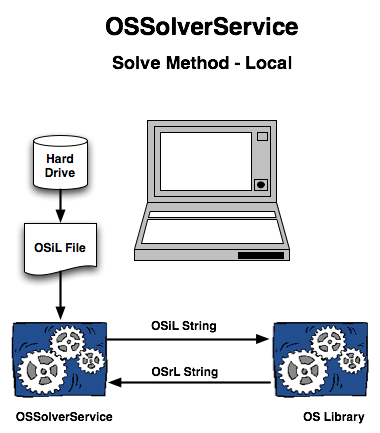
\includegraphics[scale=0.5]{\figurepath/OSSolverServiceLocal.png}
\caption{A local call to {\tt solve}.}
\label{figure:ossolverservicelocal}
\end{figure}



Here is an example of using a configure file,  {\tt testlocal.config}, to invoke {\tt Ipopt} locally using the {\tt solve} command.

\begin{verbatim}
-osil ../data/osilFiles/parincQuadratic.osil
-solver ipopt
-serviceMethod solve
-browser /Applications/Firefox.app/Contents/MacOS/firefox
-osrl /Users/kmartin/temp/test.osrl
\end{verbatim}



The first line of {\tt testlocal.config} gives the local location of the OSiL file, {\tt parincQuadratic.osil}, that contains the problem instance. The second parameter, {\tt -solver ipopt},  is the solver to be invoked, in this case COIN-OR Ipopt. The third parameter {\tt -serviceMethod solve} is not really needed, but included only for illustration. The default  solver service is {\tt solve.}  The fourth parameter is the location of the browser on the local machine. It will read the OSrL file on the local machine using the path specified by the value of the {\tt osrl} parameter, in this case {\tt /Users/kmartin/temp/test.osrl.}

Parameters may also be contained in an XML-file in OSoL format. In the configuration file {\tt testlocalosol.config} we illustrate specifying the instance location in an OSoL file.
\begin{verbatim}
-osol ../data/osolFiles/demo.osol
-solver clp
\end{verbatim}
The file {\tt demo.osol} is

\begin{verbatimtab}[4]
<?xml version="1.0" encoding="UTF-8"?>
<osol xmlns="os.optimizationservices.org">
	<general>
		<instanceLocation locationType="local">
			../data/osilFiles/parincLinear.osil
		</instanceLocation>
	</general>
</osol>
\end{verbatimtab}

\subsection{Solving Problems Remotely with Web Services}\label{section:servicemethods}

In many cases the client machine may be a ``weak client'' and  using a more powerful machine to solve a hard optimization instance is required. Indeed, one of the major purposes of Optimization Services is to facilitate optimization in a distributed environment.   We now provide examples that illustrate using the {\tt OSSolverService} executable to call a remote solver service.   By remote solver service we mean a solver service that is called using Web Services.  The OS implementation  of the solver service  uses Apache Tomcat. See \url{tomcat.apache.org}. The Web Service running on the server is a Java program based on Apache Axis. See \url{ws.apache.org/axis}. This is described in greater detail in Section \ref{section:tomcat}.  This Web Service is called {\tt OSSolverService.jws}. It is not necessary to use the Tomcat/Axis combination.



See Figure \ref{figure:ossolverservice} for an illustration of this process. The client machine uses {\tt OSSolverService} executable to call one of the six service methods, e.g. {\tt solve}. The  information such as the problem instance in OSiL format and solver options in OSoL format are packaged into a SOAP envelope and sent to the server. The server is running the Java Web Service {\tt OSSolverService.jws}. This Java program running in the Tomcat Java Servlet container implements the six service methods. If a {\tt solve} or {\tt send} request is sent to the server from the client, an optimization problem must be solved. The Java solver service solves the optimization instance by  calling the  OSSolverService on the server. So there is an OSSolverService on the client that calls the Web Service {\tt  OSSolverService.jws} that in turn calls  the executable {\tt OSSovlerService} on the server. The Java solver service passes options to the local {\tt OSSolverService} such as where the OSiL file is located and where to write the solution result.

\begin{figure}
\centering
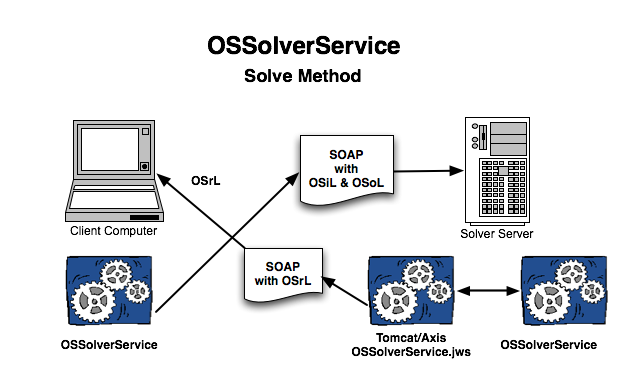
\includegraphics[scale=0.5]{\figurepath/OSSolverService.png}
\caption{A remote call to {\tt solve}.}
\label{figure:ossolverservice}
\end{figure}


In the following sections we illustrate each of the six service methods.

\subsubsection{The  {\tt solve} Service Method}\label{section:solve}

First we illustrate a simple call to  the  {\tt OSSolverService.jws}.  The call on the client machine is

\begin{verbatim}
./OSSolverService -config ../data/configFiles/testremote.config
\end{verbatim}
where the {\tt testremote.config} file is
\begin{verbatim}
-osil ../data/osilFiles/parincLinear.osil
-serviceLocation http://gsbkip.chicagogsb.edu/os/OSSolverService.jws
\end{verbatim}

No solver is specified and by default the  {\tt Cbc} solver  is used by the {\tt OSSolverService}.   If, for example, the user wished to solve the problem with the {\tt Clp} solver then this is accomplished either by using the  {\tt -solver} option on the command line
\begin{verbatim}
./OSSolverService -config ../data/configFiles/testremote.config -solver clp
\end{verbatim}
or by  adding  the line
\begin{verbatim}
 -solver clp
\end{verbatim}
to the  {\tt testremote.config} file.

Next we illustrate a call to the remote SolverService and specify an OSiL instance that is actually residing on the remote machine that is hosting the {\tt OSSolverService} and not on the client machine.
\begin{verbatim}
./OSSolverService -osol ../data/osolFiles/remoteSolve1.osol
     -serviceLocation  http://gsbkip.chicagogsb.edu/os/OSSolverService.jws
\end{verbatim}
where the {\tt remoteSolve1.osol} file is
\begin{verbatimtab}[4]
<?xml version="1.0" encoding="UTF-8"?>
<osol xmlns="os.optimizationservices.org">
    <general>
         <instanceLocation locationType="local">c:\parincLinear.osil</instanceLocation>
         <contact transportType="smtp">kipp.martin@chicagogsb.edu</contact>
    </general>
    <optimization>
    	<other name="os_solver">ipopt</other>
    </optimization>
</osol>
\end{verbatimtab}


If we were to change to the {\tt locationType} attribute in the {\tt <instanceLocation>} element to {\tt http} then we could specify the intance location to on yet another machine. This is illustrated below  for {\tt remoteSovle2.osol}.  The scenario is depicted in Figure \ref{figure:ossolverservice2}.  The OSiL string passed from the client to the solver service is empty.  However, the OSoL element {\tt <instanceLocation>}  has an attribute {\tt locationType} equal to   {\tt http}.  In this case, the text of the {\tt <instanceLoction>} element contains the URL of a third machine which has the problem intance {\tt parincLinear.osil}.  The solver service will contact the machine with URL {\tt http://www.coin-or.org/OS/parincLinear.osil} and download this test problem. So the {\tt OSSolverService} is running on the server {\tt gsbkip.chicagogsb.edu} which contacts the server {\tt www.coin-or.org} for the model instance.
\begin{verbatimtab}[4]
<?xml version="1.0" encoding="UTF-8"?>
<osol xmlns="os.optimizationservices.org">
    <general>
         <instanceLocation locationType="http">
	http://www.coin-or.org/OS/parincLinear.osil
	 </instanceLocation>
    </general>
    <optimization>
    	<other name="os_solver">ipopt</other>
    </optimization>
</osol>
\end{verbatimtab}

\begin{figure}
\centering
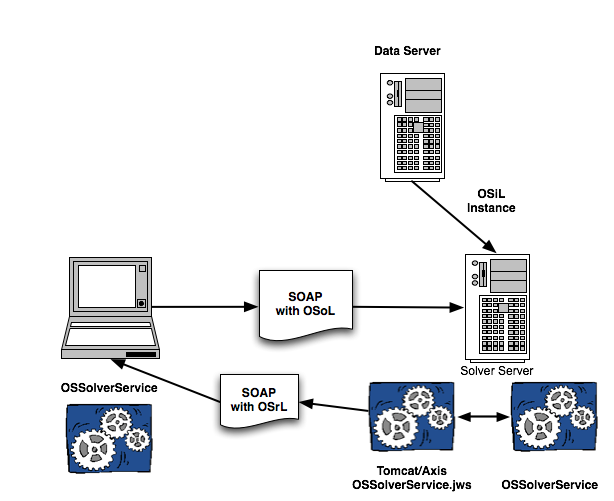
\includegraphics[scale=0.5]{\figurepath/OSSolverService2.png}
\caption{Downloading the instance from a remote source.}
\label{figure:ossolverservice2}
\end{figure}

\subsubsection{The  {\tt send} Service Method}\label{section:send}

When the {\tt solve} service method is used, the {\tt OSSolverService} does not finish execution until the solution is returned from the remote solver service. The {\tt solve} method communicates synchronously with the remote solver service. This may not be desirable for large problems when the user does not want to wait for a response. The {\tt send} service method should be used when asynchronous communication is desired. When the send method is used the instance is communicated to the remote service and the {\tt OSSolverService} terminates after submission. An example of this is
\begin{verbatim}
./OSSolverService -config ../data/configFiles/testremoteSend.config
\end{verbatim}
where the {\tt testremoteSend.config} file is
\begin{verbatim}
-nl ../data/amplFiles/hs71.nl
-serviceLocation http://gsbkip.chicagogsb.edu/os/OSSolverService.jws
-serviceMethod send
\end{verbatim}
In this example the COIN-OR {\tt Ipopt} solver is specified. The input file {\tt hs71.nl} is in AMPL format. Before sending this to the remote solver service the {\tt OSSolverService} executable converts  the nl format into the OSiL XML format and packages this into the SOAP envelope used by Web Services.

Since the {\tt send} method involves asynchronous communication the remote solver service must keep track of jobs. The send methd requires a {\tt JobID}. In the above example  no {\tt JobID} was specified. When no {\tt JobID} is specified the {\tt OSSolverService} method first invokes the {\tt getJobID} service method to get a {\tt JobID} and then puts this information into a created OSoL file and send the information to the server. More information on the {\tt getJobID} service method is provided in Section \ref{section:getjobid}.    The {\tt OSSolverService} prints the OSoL file to standard output before termination. This is illustrated below,
\begin{verbatimtab}[4]
<?xml version="1.0" encoding="UTF-8"?>
<osol xmlns="os.optimizationservices.org">
	<general>
		<jobID>
		gsbrkm4__127.0.0.1__2007-06-16T15.46.46.075-05.00149771253
		</jobID>
	</general>
    <optimization>
    	<other name="os_solver">ipopt</other>
    </optimization>
</osol>
\end{verbatimtab}
The {\tt JobID} is one that is randomly generated by the server and passed back to the {\tt OSSolverService.} The user can also provide a {\tt JobID} in their OSoL file. For example, below is a user-provided OSoL file that could be specified in a configuration file or on the command line.
\begin{verbatimtab}[4]
<?xml version="1.0" encoding="UTF-8"?>
<osol xmlns="os.optimizationservices.org">
	<general>
		<jobID>123456abcd</jobID>
	</general>
    <optimization>
    	<other name="os_solver">ipopt</other>
    </optimization>
</osol>
\end{verbatimtab}

The same {\tt JobID} cannot be used twice, so if {\tt 123456abcd} was used earlier, the result of {\tt send} will be {\tt false}.

In order to be of any use, it is necesary to get the result of the optimization. This is described in Section \ref{section:retrieve}. Before proceeding to this section, we describe two ways for knowing when the optimization is complete. One feature of the standard OS remote SolverService is the ability to send an email when the job is complete. Below is an example of the {\tt OSoL} that uses the email feature.
\begin{verbatimtab}[4]
<?xml version="1.0" encoding="UTF-8"?>
<osol xmlns="os.optimizationservices.org">
 	<general>
 		<jobID>123456abcd</jobID>
 		<contact transportType="smtp">
			kipp.martin@chicagogsb.edu
		</contact>
	</general>
    <optimization>
    	<other name="os_solver">lindo</other>
    </optimization>
</osol>
\end{verbatimtab}

The remote Solver Service will send an email to the above address when the job is complete. A second option for knowing when a job is complete is to use the knock method.

Note that in all of these examples we provided a value for the {\tt name} attribute in the {\tt <other>} element. The remote solver service will use Cbc if another solver is not specified.



\subsubsection{The  {\tt retrieve} Service Method}\label{section:retrieve}

The {\tt retrieve} has a single string argument which is an OSoL instance. Here is an example of using the {\tt retrieve} method with {\tt OSSolverService}.
\begin{verbatim}
./OSSolverService -config ../data/configFiles/testremoteRetrieve.config
\end{verbatim}
The {\tt testremoteRetrieve.config} file is
\begin{verbatim}
-serviceLocation http://gsbkip.chicagogsb.edu/os/OSSolverService.jws
-osol ../data/osolFiles/retrieve.osol
-serviceMethod retrieve
-osrl /home/kmartin/temp/test.osrl
\end{verbatim}
and the {\tt retrieve.osol} file is
\begin{verbatimtab}[4]
<?xml version="1.0" encoding="UTF-8"?>
<osol xmlns="os.optimizationservices.org">
 	<general>
 		<jobID>123456abcd</jobID>
	</general>
</osol>
\end{verbatimtab}
The OSoL file {\tt retrieve.osol} contains a tag {\tt <jobID>} that is communicated to the remote service. The remove service locates the result returns it as a string. The string that is returned is an OSrL instance.  The user must modify the line
\begin{verbatim}
-osrl /home/kmartin/temp/test.osrl
\end{verbatim}
to reflect a valid path for their own machine.  Also, the {\tt <jobID>} should reflect a {\tt <jobID>} that was previously submitted. The {\tt send()} and {\tt retrieve()}  {\tt <jobID>} must match up.

\subsubsection{The  {\tt getJobID} Service Method}\label{section:getjobid}

Before  submitting a job with the {\tt send} method a {\tt JobID} is required. The {\tt OSSolverService} can get a {\tt JobID} with
the following options.
\begin{verbatim}
-serviceLocation http://gsbkip.chicagogsb.edu/os/OSSolverService.jws
-serviceMethod getJobID
\end{verbatim}
Note that no OSoL input file is specified. In this case, the {\tt OSSolverService} sends an empty string. A string is returned with the {\tt JobID}. This {\tt JobID} is then put into a {\tt <jobID>} element in an OSoL string that would be used by the {\tt send} method.


\subsubsection{The  {\tt knock} Service Method}\label{section:knock}

The OSSolverService terminates after executing the {\tt send} method. Therefore, it is necessary to know when the job is completed on the remote server. One way is to include an email address in the  {\tt <contact>}  element with the attribute {\tt transportType}     set to {\tt smtp}.  This was illustrated in Section \ref{section:solve}.  A second way to check on the status of a job is to use the {\tt knock} service method.  For example, assume a user   wants to know if  the job with {\tt JobID 123456abcd}  is complete. A user would make the request
\begin{verbatim}
./OSSolverService -config ../data/configFiles/testRemoteKnock.config
\end{verbatim}
where the {\tt testRemoteKnock.config} file is
\begin{verbatim}
-serviceLocation http://gsbkip.chicagogsb.edu/os/OSSolverService.jws
-osplInput ../data/osolFiles/demo.ospl
-osol ../data/osolFiles/retrieve.osol
-serviceMethod knock
\end{verbatim}
the {\tt demo.ospl} file is
\begin{verbatim}
<?xml version="1.0" encoding="UTF-8"?>
<ospl xmlns="os.optimizationservices.org">
<processHeader>
<request action="getAll"/>
</processHeader>
<processData/>
</ospl>
\end{verbatim}
and the {\tt retrieve.osol} file is
\begin{verbatim}
<?xml version="1.0" encoding="UTF-8"?>
<osol xmlns="os.optimizationservices.org">
 	<general>
 		<jobID>123456abcd</jobID>
	</general>
</osol>
\end{verbatim}
The result of this request is again a string in OSpL format, with the data contained in its {\tt processData} section.  Part of the return format is illustrated below.
\begin{verbatimtab}[4]
<?xml version="1.0" encoding="UTF-8"?>
<ospl xmlns="os.optimizationservices.org">
  <processHeader>
    <serviceURI>http://localhost:8080/os/ossolver/CGSolverService.jws</serviceURI>
    <serviceName>CGSolverService</serviceName>
    <time>2006-05-10T15:49:26.7509413-05:00</time>
  <processHeader>
  <processData>
     <statistics>
        <currentState>idle</currentState>
        <availableDiskSpace>23440343040</availableDiskSpace>
        <availableMemory>70128</availableMemory>
        <currentJobCount>0</currentJobCount>
        <totalJobsSoFar>1</totalJobsSoFar>
        <timeServiceStarted>2006-05-10T10:49:24.9700000-05:00</timeServiceStarted>
        <serviceUtilization>0.1</serviceUtilization>
        <jobs>
    	  <job jobID="123456abcd">
    		<state>finished</state>
    		<serviceURI>http://gsbkip.chicagogsb.edu/ipopt/IPOPTSolverService.jws</serviceURI>
    		<submitTime>2007-06-16T14:57:36.678-05:00</submitTime>
    		<startTime>2007-06-16T14:57:36.678-05:00</startTime>
    		<endTime>2007-06-16T14:57:39.404-05:00</endTime>
    		<duration>2.726</duration>
          </job>
        </jobs>
     </statistics>
  </processData>
</ospl>
\end{verbatimtab}
Notice that the {\tt <state>} element in {\tt <job jobID="123456abcd">} indicates that the job is finished.

When making a {\tt knock} request,  the OSoL string can be empty. In this example, if the OSoL string had been empty the status of all jobs kept in the file ospl.xml is reported.  In our default solver service implementation, there is a configuration file {\tt OSParameter} that has a parameter {\tt MAX\_JOBIDS\_TO\_KEEP }.  The current default setting is 100.  In a large-scale or commercial implementation it might be wise to keep problem results and statistics in a database.  Also, there are values other than {\tt getAll} (i.e. get all process information related to the jobs) for the OSpL {\tt action} attribute in the {\tt <request>} tag.  For example, the {\tt action} can be set to a value of {\tt ping} if the user just wants to check if the remote solver service is up and running. For details, check the OSpL schema.

\subsubsection{The  {\tt kill}   Service Method}

If the user submits a job that is taking too long or is a mistake, it is possible to kill the job on the remote server using the {\tt kill} service method. For example to kill job {\tt 123456abcd}, at the command line type
\begin{verbatim}
./OSSolverService -config  ../data/configFiles/kill.config
\end{verbatim}
where the configure file {\tt kill.config} is
\begin{verbatim}
-osol ../data/osolFiles/kill.osol
-serviceLocation http://gsbkip.chicagogsb.edu/os/OSSolverService.jws
-serviceMethod kill
\end{verbatim}
and the {\tt kill.osol} file is
\begin{verbatimtab}[4]
<?xml version="1.0" encoding="UTF-8"?>
<osol xmlns="os.optimizationservices.org">
 	<general>
 		<jobID>123456abcd</jobID>
	</general>
</osol>
\end{verbatimtab}


\subsubsection{Summary}

Below is a summary of the inputs and outputs of the six service methods. See also Figure \ref{figure:osCommunicationMethods}.

\begin{itemize}
\item {\tt solve(osil, osol):}

\begin{itemize}

\item Inputs: a string with the instance in OSiL format and an optional string with the solver options in OSoL format

\item  Returns: a string with the solver solution in OSrL format

\item  Synchronous call, blocking request/response

\end{itemize}



\item {\tt send(osil, osol)}


\begin{itemize}

\item Inputs: a string with the instance in OSiL format and a string with the solver options in OSoL format (same as in {\tt solve})

\item Returns:  a boolean, true if the problem was successfully submitted, false otherwise

\item Has the same signature as {\tt solve}

\item  Asynchronous (server side), non-blocking call

\item The {\tt osol} string should have a {\tt JobID} in the {\tt <jobID>} element
\end{itemize}

\item {\tt getJobID( osol)}

\begin{itemize}

\item Inputs: a string  with the solver options in OSoL format (in this case, the string may be empty because no options are required to get the JobID)

\item  Returns: a string which is the unique job id generated by the solver service

\item  Used to maintain session and state on a distributed system
\end{itemize}



\item {\tt knock(ospl, osol)}

\begin{itemize}

\item Inputs: a string in OSpL format and an optional string with the solver options in OSoL format

\item  Returns: process and job status information from the remote server in OSpL format

\end{itemize}

\item {\tt retrieve( osol)}


\begin{itemize}

\item Inputs: a string with the solver options  in OSoL format

\item Returns: a string with the solver solution in OSrL format

\item The {\tt osol} string should have a {\tt JobID} in the {\tt <jobID>} element

\end{itemize}

\item {\tt kill( osol)}


\begin{itemize}

\item Inputs: a string with the solver options  in OSoL format

\item  Returns: process and job status information from the remote server in OSpL format

\item  Critical in long running optimization jobs

\end{itemize}

\end{itemize}



\begin{figure}[ht]
\centering
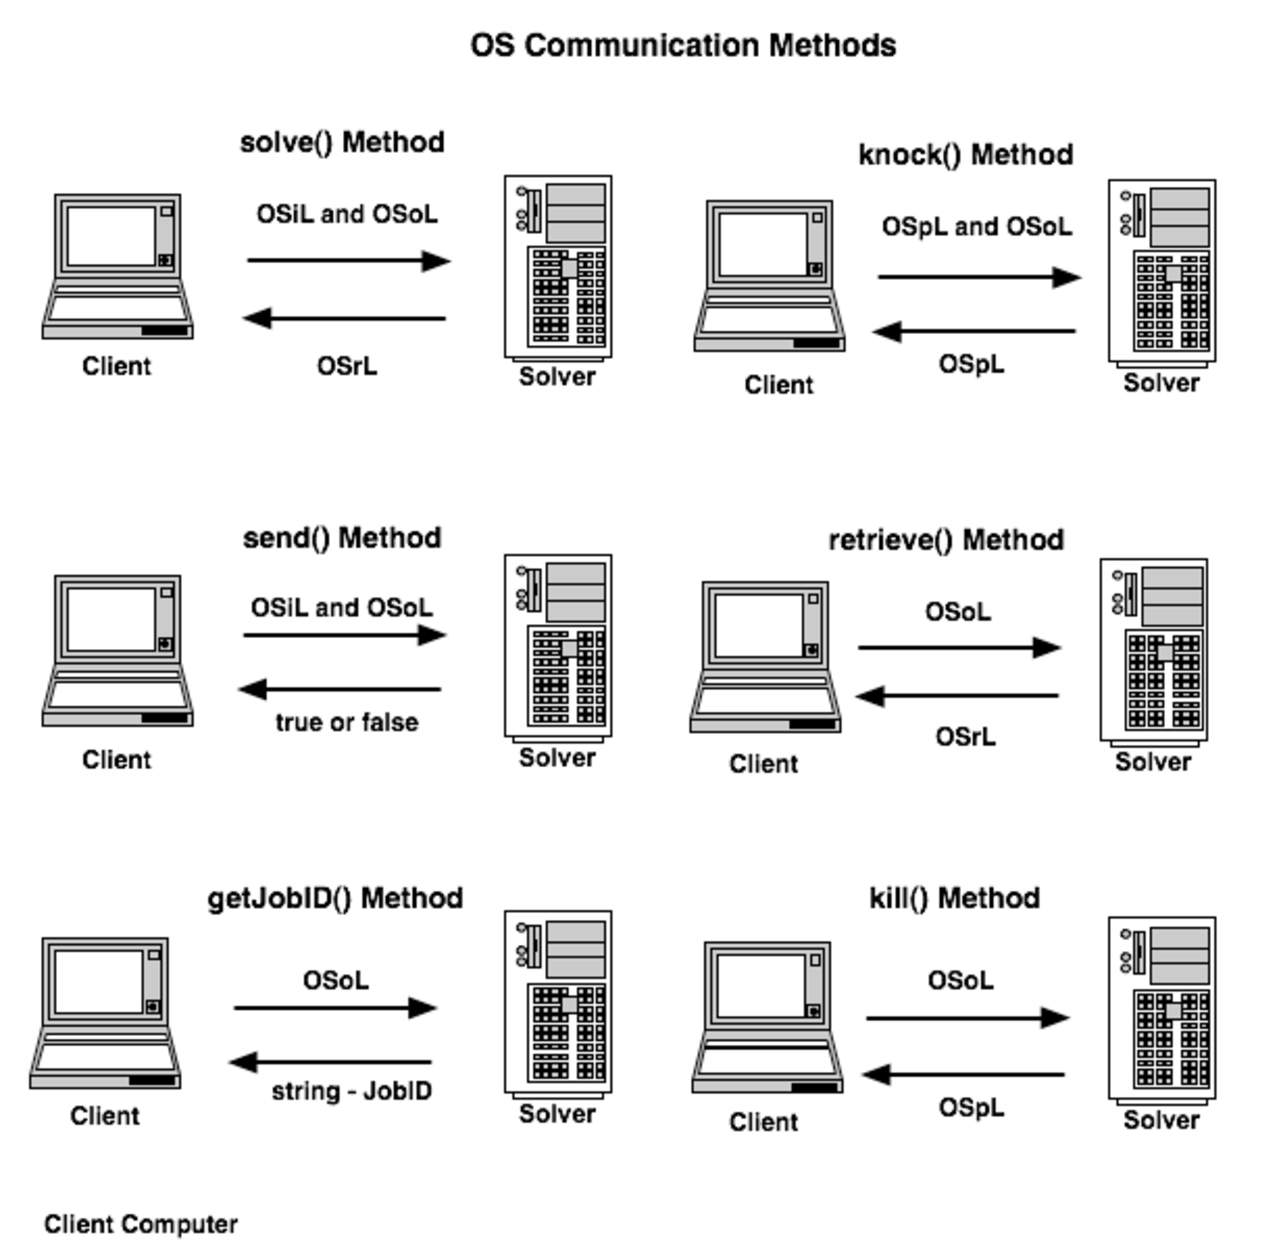
\includegraphics[scale=0.5]{\figurepath/osCommunicationMethods.pdf}
\caption{The OS Communication Methods}
\label{figure:osCommunicationMethods}
\end{figure}




\section{Setting up a Solver Service with Tomcat}\label{section:tomcat}

Download the java binary distribution at
\begin{verbatim}
os-distribution-release_number.zip
\end{verbatim}

The server side of the Java distribution is based on the Tomcat 5.5 implementation. After unpacking {\tt os-distribution-release\_number.zip} there is a directory {\tt os-server-1.0} and a single file {\tt os.war}.  For users that have not installed the Tomcat server,   {\tt os-server-1.0} contains {\tt all} of the necessary files for a OS Solver Service.  If you do not have a Tomcat server running do the following to setup a  Tomcat server  with the OS Solver Service on a {\bf Unix system}:

\begin{itemize}
\item[Step 1.]  Put the folder  {\tt os-server-1.0}   in the desired location for the OS Solver Service on the server machine.

\item[Step 2.] Connect to the Tomcat {\tt bin} directory in the {\tt os-server-1.0} root and execute {\tt ./startup.sh}.

\item[Step 3.] Test to see if the server is running the {\tt OSSolverService}.  Open a browser on the server and enter the URL
\begin{verbatim}
http://localhost:8080/os/OSSolverService.jws
\end{verbatim}
or
\begin{verbatim}
http://127.0.0.1:8080/os/OSSolverService.jws
\end{verbatim}
You should see a message {\tt Click to see the WSDL}.  Click on the link and you should see an XML description of the various methods available from the {\tt OSSolverService}.

\item[Step 4.]  On a client machine, create  the file {\tt testremote.config} with the following lines of text
\begin{verbatim}
-serviceLocation http://***.***.***.***:8080/os/OSSolverService.jws
-osil /parincLinear.osil
\end{verbatim}
where ***.***.***.*** is the IP address of the Tomcat server machine. Then, assuming the files {\tt testremote.config} and {\tt parincLinear.osil} are in the same directory on the client machine as the {\tt OSSolverService} execute:
\begin{verbatim}
./OSSolverService -config testremote.config
\end{verbatim}
You should get back an OSrL message saying the problem was optimized.

\end{itemize}

In a Windows environment you may want to start the Tomcat server as a service so you can log off (not shutdown) the machine and have the server continue to run. On a {\bf Windows machine} do the following:

\begin{itemize}

\item[Step 1.]  Put the folder  {\tt os-server-1.0}   in the desired location for the OS Solver Service on the server machine.

\item[Step 2.]  Connect to the Tomcat {\tt bin} directory in the {\tt os-server-1.0} root and execute
\begin{verbatim}
service.bat install
\end{verbatim}
This will install Tomcat as a Windows service.  To remove the service execute
\begin{verbatim}
service.bat remove
\end{verbatim}

\item[Step 3.]  Connect to the Tomcat {\tt bin} directory and and double click on the {\tt tomcat5w.exe} application.  This will open a Window for controlling the Tomcat server.

\item[Step 4.]  Select the {\tt Startup} tab and set the {\tt Working Directory} to the path to {\tt os-server-1.0}.

\item[Step 5.]  Select the {\tt General} tab and then click the {\tt Start} button.

\item[Step 6.] Same as Step 3 for Unix.

\item[Step 7:] Same as Step 4 for Unix.

\end{itemize}

\vskip 8pt

\noindent {\bf Note:}
There are many ways to start the Tomcat server and the exact way you choose may be different. See \url{http://tomcat.apache.org/} and check out Tomcat version 5.5 for more detail. But do remember to properly set the {\tt Tomcat Working Directory} to the path to {\tt os-server-1.0}. By default, if you start Tomcat on Windows, the {\tt Working Directory} is set to the Windows system folder, which will yield unpredictable results.

\vskip 8pt

If you already have a Tomcat server with Axis installed do the following:
\begin{itemize}
\item[1.] copy the file {\tt os.war} into the Tomcat {\tt WEB-INF} directory in the {\tt ROOT} folder under {\tt webapps}.

\item[2.]  Follow Steps 2-5 outlined above.
\end{itemize}

In the directory,
\begin{verbatim}
os-server-1.0/webapps/os/WEB-INF/code/OSConfig
\end{verbatim}
there is a configuration file {\tt OSParameter.xml} that can be modified to fit individual user needs. You can configure such parameters as service name, service URL/URI. Refer to the xml file for more detail. Descriptions for all the parameters are within the file itself.

\vskip 8pt

Below is a summary of the common and important directories and files you may want to know.

\begin{itemize}
\item
\begin{verbatim}
os-server-1.0/webapps/os/
\end{verbatim}
contains the OS Web application. All directories and files outside of this folder are Tomcat server related.
\item
\begin{verbatim}
os-server-1.0/webapps/os/WEB-INF
\end{verbatim}
contains private and important os configuration, library, class and executable files to run the Optimization Service. All files and directories outside of this folder but within the {\tt /os} Web application folder are publicly viewable (e.g. Web pages).
\item
\begin{verbatim}
os-server-1.0/webapps/os/WEB-INF/code/OSConfig
\end{verbatim}
contains configuration files for Optimization Services, such as the {\tt OSParameter.xml} file.
\item
\begin{verbatim}
os-server-1.0/webapps/os/WEB-INF/code/temp
\end{verbatim}
contains temporarily saved files such as submitted OSiL/OSoL input files, and OSrL output files. This folder can get bigger as the service starts to run more jobs. For maintenance purpose, you may want to keep an eye on it.
\item
\begin{verbatim}
os-server-1.0/webapps/os/WEB-INF/code/log
\end{verbatim}
contains log files from the running services in the current Web application.
\item
\begin{verbatim}
os-server-1.0/webapps/os/WEB-INF/code/solver
\end{verbatim}
contains solver binaries that actually carry out the optimization process.
\item
\begin{verbatim}
os-server-1.0/webapps/os/WEB-INF/code/backup
\end{verbatim}
contains backup files from some of the above directories. This folder can get bigger as the service starts to run more jobs. For maintenance purpose, you may want to keep an eye on it.
\item
\begin{verbatim}
os-server-1.0/webapps/os/WEB-INF/classes
\end{verbatim}
contains class files to run the Optimization Services.
\item
\begin{verbatim}
os-server-1.0/webapps/os/WEB-INF/lib
\end{verbatim}
contains library files needed by the Optimization Services.
\item
\begin{verbatim}
os-server-1.0/conf
\end{verbatim}
contains configuration files for the Tomcat server, such as http server port.
\item
\begin{verbatim}
os-server-1.0/bin
\end{verbatim}
contains executables and scripts to start and shutdown the Tomcat server.
\end{itemize}




\section{Examples}\label{section:examples}

\subsection{AMPL Client:  Hooking AMPL to Solvers}\label{section:amplclient}

The {\tt amplClient} executable (in {\tt COIN-OS/OS/examples/amplClient}) is designed to work with the AMPL program. See \url{www.ampl.com}. The {\tt amplClient} acts like an AMPL ``solver.'' The {\tt amplClient} is linked with the OS library and can be used to solve problems either locally or remotely. In both cases the {\tt amplClient} uses the {\tt OSnl2osil} class to convert the AMPL generated nl file (which represents the problem instance) into the corresponding instance representation in the OSiL format.

In the following discussion we assume that the AMPL executable {\tt ampl} obtained from {\tt www.ampl.com}, the OS {\tt amplClient}, and the test problem {\tt hs71.mod} are all in the same directory. At first, the user may wish to run everything in the directory

\begin{verbatim}
COIN-OS/OS/examples/amplClient
\end{verbatim}
which is where {\tt amplClient} is located when the OS project is built. The user must obtain {\tt ampl} and put it in this directory.  The test problem {\tt hs71.mod} can be copied from

\begin{verbatim}
COIN-OS/OS/data/amplFiles
\end{verbatim}
It is also assumed that {\tt .} (the current directory) is in the search path.

Assume that the  problem instance, {\tt hs71.mod} is in AMPL model format. To solve this problem locally by calling the {\tt amplClient} from AMPL first start AMPL and then execute the following commands. In this case we testing  {\tt Ipopt} as the local server and therefore it is necessary that {\tt Ipopt} be part of the local OS build. If it is not then another solver must be selected and a test problem used that is a linear or integer program.

\begin{verbatim}
# take in problem 71 in Hock and Schittkowski
# assume the problem is in the AMPL directory
model hs71.mod;
# tell AMPL that the solver is amplClient
option solver amplClient;
# now tell amplClient to use Ipopt
option amplClient_options "solver ipopt";
# the name of the nl file (this is optional)
write gtestfile;
# now solve the problem
solve;
\end{verbatim}

This will invoke {\tt Ipopt} locally and the result in OSrL format will be displayed on the screen. In order to call a remote solver service, after the command
\begin{verbatim}
option amplClient_options "solver ipopt";
\end{verbatim}
Next set the solver {\tt service} option to  the address of the remote solver service.
\begin{verbatim}
option ipopt_options "service http://gsbkip.chicagogsb.edu/os/OSSolverService.jws";
\end{verbatim}
In this case it is necessary that the {\tt Ipopt} solver be part of the OS build on the server.

\subsection{Algorithmic Differentiation:  Using the OS Algorithmic Differentiation Methods}\label{section:cppad}

In the {\tt OS/examples/algorithmicDiff} folder is test code {\tt algorithmicDiffTest.cpp}. This code illustrates the key methods in the {\tt OSInstance} API that are used for algorithmic differentiation.   These methods were described in Section \ref{section:ad}.



\subsection{File Upload:  Using a File Upload Package}\label{section:fileupload}



When the {\tt OSAgent}  class methods {\tt solve} and {\tt send} are used, the problem instance in OSiL format is packaged into a SOAP envelope and communication with the server is done using Web Services (for example Tomcat Axis). However, packing an XML file into a SOAP envelope may add considerably to the size of the file (each {\tt $<$} is replaced with {\tt \&lt;}  and each {\tt $>$} is replaced with {\tt \&gt;}). Also, communicating with a Web Services servlet can also slow down the communication process. This could be a problem for large instances. An alternative approach is to use the {\tt fileUpload} executable on the client end  and the Java servlet {\tt OSFileUpload} on the server end.  The {\tt fileUpload} client executable is contained in the {\tt fileUpload}  directory inside the {\tt examples directory}.

This servlet is based upon the Apache Commons FileUpload. See \url{http://jakarta.apache.org/commons/fileupload/}. The {\tt OSFileUpload} Java class , {\tt OSFileUpload.class} is in the directory
\begin{verbatim}
webapps\os\WEB-INF\classes\org\optimizationservices\oscommon\util
\end{verbatim}
relative to the Web server root.  The source code {\tt OSFileUpload.class} is in the directory
\begin{verbatim}
 COIN-OS/OS/examples/fileUpload
 \end{verbatim}



The {\tt fileUpload} client executable ((see {\tt OS/examples/fileUpload})) takes one argument on the command line which is the location of the file on the local directory to upload to the server. For example,
\begin{verbatim}
fileUpload ../../data/osilFiles/parincQuadratic.osil
\end{verbatim}
The {\tt fileUpload} executable first creates an {\tt OSAgent} object.
\begin{verbatim}
OSSolverAgent* osagent = NULL;
osagent = new OSSolverAgent("http://gsbkip.chicagogsb.edu/fileupload/servlet/OSFileUpload");
\end{verbatim}
The {\tt OSAgent}  has a method {\tt fileUpload} with the signature
\begin{verbatim}
std::string fileUpload(std::string osilFileName, std::string osil);
\end{verbatim}
where {\tt osilFileName} is  the name of the OSiL problem instance to be written on the server and {\tt osil} is the string with the actual instance. Then
\begin{verbatim}
osagent->fileUpload(osilFileName, osil);
\end{verbatim}
will place a call to the server, upload the problem instance in the {\tt osil} string, and cause the server to write a file on its hard drive named {\tt osilFileName}. In our implementation, the uploaded file ({\tt parincQuadratic.osil}) is saved to the {\tt/home/kmartin/temp/parincQuadratic.osil} on the server hard drive. This location is used in the {\tt osol} file as shown below.

Once the file is on the server, invoke the local {\tt OSSolverService} by
\begin{verbatim}
./OSSolverService -config ../data/configFiles/testremote.config
\end{verbatim}
where the {\tt config} file is as follows. Notice there is no {\tt -osil}  option as the osil file has already been uploaded and its instance location ("local" to the server) is specified in the {\tt osol} file.
\begin{verbatim}
-osol ../data/osolFiles/remoteSolve2.osol
-serviceLocation http://gsbkip.chicagogsb.edu/os/OSSolverService.jws
-serviceMethod solve
\end{verbatim}
and the {\tt osol} file is
\begin{verbatimtab}[5]
<osol>
    <general>
         <instanceLocation locationType="local">
         	/home/kmartin/temp/parincQuadratic.osil
         </instanceLocation>
    </general>
    <optimization>
    	<other name="os_solver">ipopt</other>
    </optimization>
</osol>
\end{verbatimtab}

As an alternative to using the command line executable {\tt fileUpload}, there is also an html form {\tt fileupload.html} that can be used to upload files. For example, the URL
\begin{verbatim}
http://gsbkip.chicagogsb.edu/os/fileupload.html
\end{verbatim}
will bring up the necessary form that allows the user to browse a directory and select the file to upload. This URL is based on the assumption that the {\tt OSJava} classes were deployed as described in Section \ref{section:tomcat}. The file {\tt fileupload.html} is in the directory {\tt WebApps/os}. In our html form implementation, after you upload the OSiL file, it shows you the path of the uploaded file that is saved on the server, so that you can put it in the corresponding {\tt osol} file.




\subsection{Instance Generator: Using the OSInstance API to Generate Instances}\label{subsection:exampleOSInstanceGeneration}

This example is found in the {\tt instanceGenerator} folder in the {\tt examples} folder.  This example illustrates how to build a complete in-memory model instance using the {\tt OSInstance} API.   See the code {\tt instanceGenerator.cpp} for the complete example. Here we provide a few highlights to illustrate the power of the API.

The first step is to create an {\tt OSInstance} object.
\begin{verbatim}tt
OSInstance *osinstance;
osinstance = new OSInstance();
\end{verbatim}

Assume that the instance has two variables, $x_{0}$ and $x_{1}.$ Variable $x_{0}$ is a continuous variable with lower bound of -100 and upper bound of 100. Variable $x_{1}$ is a binary variable. First declare the instance to have two variables.
\begin{verbatim}
osinstance->setVariableNumber( 2);
\end{verbatim}
Next, add each variable. There is an {\tt addVariable} method with the signature
\begin{verbatim}
addVariable(int index, string name, double lowerBound, double upperBound,
char type, double init, string initString);
\end{verbatim}
Then the calls for these two variables are
\begin{verbatim}
osinstance->addVariable(0, "x0", -100, 100, 'C', OSNAN, "");
osinstance->addVariable(1, "x1", 0, 1, 'B', OSNAN, "");
\end{verbatim}
There is also a method {\tt setVariables} for adding more than one variable simultaneously.  The objective function(s) and constraints are added through similar calls.

Nonlinear terms are also easily added.  The following code illustrates how to add a nonlinear term $x_{0}*x_{1}$ in the {\tt <nonlinearExpressions>} section of  OSiL.
\begin{verbatim}
osinstance->instanceData->nonlinearExpressions->nl[ 1] = new Nl();
osinstance->instanceData->nonlinearExpressions->nl[ 1]->idx = 1;
osinstance->instanceData->nonlinearExpressions->nl[ 1]->osExpressionTree =
new OSExpressionTree();
// create a variable nl node for x0
nlNodeVariablePoint = new OSnLNodeVariable();
nlNodeVariablePoint->idx=0;
nlNodeVec.push_back( nlNodeVariablePoint);
// create the nl node for x1
nlNodeVariablePoint = new OSnLNodeVariable();
nlNodeVariablePoint->idx=1;
nlNodeVec.push_back( nlNodeVariablePoint);
// create the nl node for *
nlNodePoint = new OSnLNodeTimes();
nlNodeVec.push_back( nlNodePoint);
// the vectors are in postfix format
// now the expression tree
osinstance->instanceData->nonlinearExpressions->nl[ 1]->osExpressionTree->m_treeRoot =
nlNodeVec[ 0]->createExpressionTreeFromPostfix( nlNodeVec);
\end{verbatim}

\subsection{osTestCode}\label{subsection:exampleOSInstanceGeneration}

The {\tt osTestCode} example directory holds the file {\tt osTestCode.cpp}. This is not designed to do anything specific and is simply a holder for testing out code and features of the OS library.

\section{Appendix}\label{section:appendix}


\subsection{Building a Model in MATLAB}

We illustrate how to build a simple Markowitz portfolio optimization problem (a quadratic programming problem) from {\bf template.m}. First copy {\bf template.m} to {\bf markowitz.m}.

Assume that there are three stocks (variables) and two constraints (do not count the upper limit investment of .75 on the variables.).


\begin{verbatim}
% the number of constraints
numCon = 2;
% the number of variables
numVar = 3;
\end{verbatim}



All the variables are continuous


\begin{verbatim}
VarType='CCC';
\end{verbatim}


Next define the constraint upper and lower bounds. There are two constraints. A unity constraint (an $=$) and a lower bound on portfolio return of .15 (a $\ge$). These two constraints are expressed as



\begin{verbatim}
BU = [1  inf];
BL = [1   .15];
\end{verbatim}



The variables are nonnegative and have upper limits of .75 (no stock can comprise more than 75\% of the portfolio).  This is written as




\begin{verbatim}
VL = [];
VU = [.75 .75 .75];
\end{verbatim}



There are no nonzero linear coefficients in the objective function, but the objective function vector must always be defined and the number of components of this vector is the number of variables.



\begin{verbatim}
OBJ = [0 0 0 ]
\end{verbatim}


 Now the linear constraints.   In the model the two linear constraints are
 \begin{eqnarray*}
 0.3221 x_{1} +   0.0963x_{2} +    0.1187x_{3}  &\ge& .15 \\
x_{1} + x_{2} + x_{3} &=& 1
 \end{eqnarray*}



 These are expressed as



 \begin{verbatim}
 A = [ 1 1 1  ;
  0.3221   0.0963   0.1187 ];
 \end{verbatim}


Now for the quadratic terms. The only quadratic terms are in the objective function. The objective function is


\begin{eqnarray*}
\min  0.4253 x_{1}^{2} +  0.4458 x_{2}^{2} + 0.2314 x_{3}^{2} + 2 \times 0.1852 x_{1} x_{2} \\ + 2 \times 0.1393 x_{1} x_{3} + 2 \times
 0.1388 x_{2} x_{3}
\end{eqnarray*}


 The quadratic matrix $Q$ has 4 rows and a column for each quadratic term. In this example there are six quadratic terms.  The first row of $Q$ is the row index where the terms appear. By convention, the objective function has index -1 and we count constraints starting at 0.  The first row of $Q$ is


 \begin{verbatim}
 -1 -1 -1 -1 -1 -1
 \end{verbatim}

The second row of $Q$ is the index of the first variable in the quadratic term. We use zero based counting.  Variable $x_{1}$ has index, variable  $x_{2}$ has index 1, and variable $x_{3}$ has index 2.  Therefore, the second row of $Q$ is



\begin{verbatim}
0 1 2 0 0 1
\end{verbatim}



The third row of $Q$ is the index of the second variable in the quadratic term.   Therefore, the third row of $Q$ is



\begin{verbatim}
0 1 2  1 2 2
\end{verbatim}



The last (fourth) row is the coefficient. Therefore, the fourth row is





\begin{verbatim}
 .425349654  .445784443   0.231430983
 .370437388  .27862509 .27763384
\end{verbatim}


The quadratic matrix is



\begin{verbatim}
Q = [ -1 -1 -1 -1 -1 -1;
0 1 2 0 0 1 ;
0 1 2 1 2 2;
.425349654  .445784443   0.231430983   ...
.370437388  .27862509 .27763384];
\end{verbatim}


Finally, name the problem, specify the solver (in this case {\tt ipopt}), the service address (and password if required by the service), and call the solver.



\begin{verbatim}
prob_name = 'Markowitz Example from Anderson, Sweeney, Williams, and Martin'
password = 'chicagoesmuyFRIO';
%
%the solver
solverName = 'ipopt';
%the remote service service address
%if left empty we solve locally
serviceAddress='http://gsbkip.chicagogsb.edu/os/OSSolverService.jws';
% now solve
callMatlabSolver( numVar, numCon, A, BL, BU, OBJ, VL, VU, ObjType, VarType, ...
     Q, prob_name, password, solverName, serviceAddress)
\end{verbatim}




\subsection{OSiL representation for problem given in
(\ref{eq:roobj})--(\ref{eq:ro3})}\label{section:rosenbrockXML}


{\normalsize \baselineskip 16pt \vspace{2pt}
\begin{verbatimtab}[5]
<?xml version="1.0" encoding="UTF-8"?>
<osil xmlns="os.optimizationservices.org">
	<instanceHeader>
		<name>Modified Rosenbrock</name>
		<source>Computing Journal 3:175-184, 1960</source>
		<description>Rosenbrock problem with constraints</description>
	</instanceHeader>
	<instanceData>
		<variables numberOfVariables="2">
			<var lb="0" name="x0" type="C"/>
			<var lb="0" name="x1" type="C"/>
		</variables>
		<objectives numberOfObjectives="1">
			<obj maxOrMin="min" name="minCost" numberOfObjCoef="1">
				<coef idx="1">9.0</coef>
			</obj>
		</objectives>
		<constraints numberOfConstraints="2">
			<con ub="25.0"/>
			<con lb="10.0"/>
		</constraints>
		<linearConstraintCoefficients numberOfValues="3">
			<start>
				<el>0</el><el>2</el><el>3</el>
			</start>
			<rowIdx>
				<el>0</el><el>1</el><el>1</el>
			</rowIdx>
			<value>
				<el>1.</el><el>7.5</el><el>5.25</el>
			</value>
		</linearConstraintCoefficients>
		<quadraticCoefficients numberOfQuadraticTerms="3">
			<qTerm idx="0" idxOne="0" idxTwo="0" coef="10.5"/>
			<qTerm idx="0" idxOne="1" idxTwo="1" coef="11.7"/>
			<qTerm idx="0" idxOne="0" idxTwo="1" coef="3."/>
		</quadraticCoefficients>
\end{verbatimtab}
   \newpage
\begin{verbatimtab}[5]
		<nonlinearExpressions numberOfNonlinearExpressions="2">
			<nl idx="-1">
				<plus>
					<power>
						<minus>
							<number type="real" value="1.0"/>
							<variable coef="1.0" idx="0"/>
						</minus>
						<number type="real" value="2.0"/>
					</power>
					<times>
						<power>
							<minus>
								<variable coef="1.0" idx="0"/>
								<power>
									<variable coef="1.0" idx="1"/>
									<number type="real" value="2.0"/>
								</power>
							</minus>
							<number type="real" value="2.0"/>
						</power>
						<number type="real" value="100"/>
					</times>
				</plus>
			</nl>
			<nl idx="1">
				<ln>
					<times>
						<variable coef="1.0" idx="0"/>
						<variable coef="1.0" idx="1"/>
					</times>
				</ln>
			</nl>
		</nonlinearExpressions>
	</instanceData>
</osil>
\end{verbatimtab}

}% end


\subsection{OSiL representation for problem given in (\ref{eq:adobj})--(\ref{eq:adeq2})}\label{section:adexample}

\begin{verbatimtab}
<?xml version="1.0" encoding="UTF-8"?>
<osil xmlns="os.optimizationservices.org"
xmlns:xsi="http://www.w3.org/2001/XMLSchema-instance"
xsi:schemaLocation="os.optimizationservices.org
http://www.optimizationservices.org/schemas/OSiL.xsd">
	<instanceHeader>
		<description>A test problem for Algorithmic Differentiation</description>
	</instanceHeader>
	<instanceData>
		<variables numberOfVariables="4">
			<var lb="0" name="x0" type="C"/>
			<var lb="0" name="x1" type="C"/>
			<var lb="0" name="x2" type="C"/>
			<var lb="0" name="x3" type="C"/>
		</variables>
		<objectives numberOfObjectives=" 1">
			<obj maxOrMin="min" name="minCost" numberOfObjCoef="1">
				<coef idx="1">9.0</coef>
			</obj>
		</objectives>
		<constraints numberOfConstraints="2">
			<con ub="10.0" constant="33"/>
			<con lb="10.0"/>
		</constraints>
		<linearConstraintCoefficients numberOfValues="2">
			<start>
				<el>0</el>
				<el>0</el>
				<el>1</el>
				<el>1</el>
				<el>2</el>
			</start>
			<rowIdx>
				<el>0</el>
				<el>1</el>
			</rowIdx>
			<value>
				<el>5</el>
				<el>7</el>
			</value>
		</linearConstraintCoefficients>
		<nonlinearExpressions numberOfNonlinearExpressions="3">
			<nl idx="1">
				<ln>
					<times>
						<variable coef="1.0" idx="0"/>
						<variable coef="1.0" idx="2"/>
					</times>	
				</ln>
			</nl>
			<nl idx="0">
				<sum>
					<number type="real" value="-105"/>
					<variable coef="1.37" idx="1"/>
					<variable coef="2" idx="2"/>
				</sum>	
			</nl>
			<nl idx="-1">
				<power>
					<variable coef="1.0" idx="0"/>
					<number type="real" value="2.0"/>
				</power>
			</nl>
		</nonlinearExpressions>
	</instanceData>
</osil>
\end{verbatimtab}


\bibliography{\bibpath/kippbib}

\end{document}

Here is where you get winsock.h


ftp://sunsite.unc.edu/pub/micro/pc-stuff/ms-windows/winsock/winsock-1.1/winsock.h

see also

ftp://sunsite.unc.edu/pub/micro/pc-stuff/ms-windows/winsock/winsock-1.1/


For the SDK (windows.h)

http://www.microsoft.com/downloads/details.aspx?FamilyId=A55B6B43-E24F-4EA3-A93E-40C0EC4F68E5&displaylang=en#Instructions


Important comments from Lou:

	Using Coin-All as of late afternoon (up-to-date, according to svn
update), and after installing the SDK as per Andreas' email, I have a `minimal
Msys' build using cl, with ASL, and OS, but it's definitely not clean. Here are
the issues, and the workarounds I used.

	Cbc.exe doesn't link with ampl in the mix, and I put the blame on
amplsolv.lib. MS link reports a conflict, apparently libcmt.lib and libcmtd.lib
(normal and debugging malloc, respectively) are both pulled in. There's a fix:
The link message says `use NODEFAULTLIB', and sure enough, if I edit the
Makefile to read

 $(CXXLINK) $(cbc_LDFLAGS) $(cbc_OBJECTS) $(cbc_LDADD) $(LIBS) \
   "-link -NODEFAULTLIB:libcmt.lib"

then cbc.exe will link. The quotes are necessary because the cl mechanism for
passing things to the linker is `everything on the line after -link', and
without the quotes libtool rearranges things. I don't know enough about MSVS
defaults to say whether libcmtd is the default on a debug build, or libcmt. JP
might have some insight. I have no immediate ideas on how to work this hack
through autotools from a Makefile.am. Might be easier to fix amplsolv.lib.

	The same hack is necessary to link OSSolverService.exe, the OS
unitTest.exe, and the OS amplClient.exe.

	When building OSAgent, the -I/include and -I/mingw/include have to go.
The cl include order is `current directory, -I options, INCLUDE environment
variable.' When either of /include or /mingw/include are specified with -I,
MinGW include files are selected first, and they're not compatible with MS
include files.

	I didn't run into the problem Ted describes, but that's probably
because I'm doing static links and the function (CbcOrClpReadCommand) is never
used anywhere except in cbc.exe. Link is bright enough to know it doesn't need
it.

	The Alps unit test crashes. Which is odd because the Bcps and Blis unit
tests run just fine.

	The OS unit test runs until it gets to the Ampl testing section,
and dies because it can't find parinc.nl. I'm not an Ampl user --- is a .nl
file Ampl output? If so, the result makes sense, because I don't have Ampl on
this machine.

	While we're here, the -rpath <path> going into libtool seems to
translate into an attempt to pass -L<path> to cl, which it ignores with a
warning about an invalid option.  Whatever libtool is hoping to achieve, it's
failing. And not necessary, apparently, at least for a static build.
	
%%%%

Important comments from Andreas:



This is a well-known problem with the free cl compiler.  I had the same problem and search the web.

This is what I believe I did:

Download and install the (free) SDK, which has the missing header files:

http://www.microsoft.com/downloads/details.aspx?FamilyId=0BAF2B35-C656-4969-ACE8-E4C0C0716ADB&displaylang=en

or so.

After that, there was still something wrong with the PATH setup for cl.  I edited my

/media/win/c/Program Files/Microsoft Visual Studio 8/Common7/Tools/vsvars32.bat

file so that the INCLUDE variable includes the correct path to the SDK include files, something like:

@set PATH=C:\Program Files\Microsoft Visual Studio 8\Common7\IDE;C:\Program Files\Microsoft Visual Studio 8\VC\BIN;C:\Program Files\Microsoft Visual Studio 8\Common7\Tools;C:\Program Files\Microsoft Visual Studio 8\SDK\v2.0\bin;C:\WINDOWS\Microsoft.NET\Framework\v2.0.50727;C:\Program Files\Microsoft Visual Studio 8\VC\VCPackages;C:\Program Files\Microsoft Platform SDK\Bin;%PATH%
@set INCLUDE=C:\Program Files\Microsoft Visual Studio 8\VC\INCLUDE;C:\Program Files\Microsoft Platform SDK\Include;%INCLUDE%
@set LIB=C:\Program Files\Microsoft Visual Studio 8\VC\LIB;C:\Program Files\Microsoft Visual Studio 8\SDK\v2.0\lib;C:\Program Files\Microsoft Platform SDK\Lib%LIB%
@set LIBPATH=C:\WINDOWS\Microsoft.NET\Framework\v2.0.50727

There are a number of discussions about this on the web, e.g.

http://www.gamedev.net/community/forums/topic.asp?topic_id=440340

I hope this helps,

%%%%%%

Andreas bug report:

<!DOCTYPE html
    PUBLIC "-//W3C//DTD XHTML 1.0 Strict//EN"
    "http://www.w3.org/TR/xhtml1/DTD/xhtml1-strict.dtd">
<html xmlns="http://www.w3.org/1999/xhtml" lang="en" xml:lang="en">
<head>
 <title>#3 (Problem compiling on AIX (CppAD trouble?)) - Optimization Services - Trac</title><link rel="start" href="/OS/wiki" /><link rel="search" href="/OS/search" /><link rel="help" href="/OS/wiki/TracGuide" /><link rel="stylesheet" href="/OS/chrome/common/css/trac.css" type="text/css" /><link rel="stylesheet" href="/OS/chrome/common/css/ticket.css" type="text/css" /><link rel="icon" href="/OS/chrome/common/trac.ico" type="image/x-icon" /><link rel="shortcut icon" href="/OS/chrome/common/trac.ico" type="image/x-icon" /><link rel="alternate" href="/OS/ticket/3?format=rss" title="RSS Feed" type="trac.ticket.Ticket" /><link rel="alternate" href="/OS/ticket/3?format=tab" title="Tab-delimited Text" type="trac.ticket.Ticket" /><link rel="alternate" href="/OS/ticket/3?format=csv" title="Comma-delimited Text" type="trac.ticket.Ticket" /><style type="text/css">
</style>
 <script type="text/javascript" src="/OS/chrome/common/js/trac.js"></script>
</head>
<body>


<div id="banner">

<div id="header"><a id="logo" href="http://www.coin-or.org/"><img src="/OS/chrome/common/coin_banner.jpg" width="80" height="80" alt="" /></a><hr /></div>

<form id="search" action="/OS/search" method="get">
 <div>
  <label for="proj-search">Search:</label>
  <input type="text" id="proj-search" name="q" size="10" accesskey="f" value="" />
  <input type="submit" value="Search" />
  <input type="hidden" name="wiki" value="on" />
  <input type="hidden" name="changeset" value="on" />
  <input type="hidden" name="ticket" value="on" />

 </div>
</form>



<div id="metanav" class="nav"><ul><li class="first"><a href="/OS/login">Login</a></li><li><a href="/OS/settings">Settings</a></li><li><a accesskey="6" href="/OS/wiki/TracGuide">Help/Guide</a></li><li><a href="/OS/about">About Trac</a></li><li class="last"><a href="/OS/register">Register</a></li></ul></div>
</div>

<div id="mainnav" class="nav"><ul><li class="first"><a accesskey="1" href="/OS/wiki">Wiki</a></li><li><a accesskey="2" href="/OS/timeline">Timeline</a></li><li><a accesskey="3" href="/OS/roadmap">Roadmap</a></li><li><a href="/OS/browser">Browse Source</a></li><li class="active"><a href="/OS/report">View Tickets</a></li><li class="last"><a accesskey="4" href="/OS/search">Search</a></li></ul></div>

<div id="main">




<div id="ctxtnav" class="nav">
 <h2>Ticket Navigation</h2>
</div>

<div id="content" class="ticket">

 <h1>Ticket #3 <span class="status">(new defect)</span></h1>

<div id="searchable">
<div id="ticket">
 <div class="date">
  <p title="08/10/07 12:53:44">Opened 1 week ago</p>
 </div>
 <h2 class="summary">Problem compiling on AIX (CppAD trouble?)</h2>
 <table class="properties">
  <tr>

   <th id="h_reporter">Reported by:</th>
   <td headers="h_reporter">andreasw</td>
   <th id="h_owner">Assigned to:</th>
   <td headers="h_owner">somebody</td>
  </tr><tr>
    <th id="h_priority">Priority:</th>

    <td headers="h_priority">major</td>
    <th id="h_milestone">Milestone:</th>
    <td headers="h_milestone"></td></tr><tr>
    <th id="h_component">Component:</th>
    <td headers="h_component">component1</td>
    <th id="h_version">Version:</th>

    <td headers="h_version"></td></tr><tr>
    <th id="h_keywords">Keywords:</th>
    <td headers="h_keywords"></td>
    <th id="h_cc">Cc:</th>
    <td headers="h_cc"></td></tr><tr></tr>
 </table>
  <form method="get" action="/OS/ticket/3#comment" class="printableform">
   <div class="description">

    <h3 id="comment:description">
     Description
    </h3>
    <p>
I'm trying to compile on AIX (IBM's xlC compiler).
</p>
<p>
The first set of problems comes in because CppAD is using the identifiers "isfinite" and "isnan", which on AIX is the name of preprocessor macros, defined in /usr/include/math.h.  I got around this problem buy renaming "isfinite" and "isnan" in CppAD's near_equal.hpp and nan.hpp.  But maybe the issue is related that you use &lt;math.h&gt; in C++ code, whereas the C++ standard says you should use &lt;cmath&gt;.  In Ipopt, I check for each C header if the C++ version is there, and if not, if the C version is there, and include the files accordingly.  There is macro for testing in coin.m4.  In Ipopt's configure.ac I use:
</p>

<pre class="wiki">AC_COIN_CHECK_CXX_CHEADER(math)
</pre><p>
and then the source code has:
</p>
<pre class="wiki">#ifdef HAVE_CMATH
# include &lt;cmath&gt;
#else
# ifdef HAVE_MATH_H
#  include &lt;math.h&gt;
# else
#  error "don't have header file for math"
# endif
#endif
</pre><p>
Once I'm able to get through that point, I get tons of error messages like the following:
</p>
<pre class="wiki">"/u/andreasw/home4/COIN-svn/CoinAll/branches/all-trunk/cppad/../cppad/local/std_math_unary.hpp", line 322.9: 1540-0215 (S) The wrong number of arguments have been specified for "CppAD::AD&lt;double&gt;::cos() const".
"/u/andreasw/home4/COIN-svn/CoinAll/branches/all-trunk/cppad/../cppad/local/std_math_unary.hpp", line 322.9: 1540-0700 (I) The previous message was produced while processing "CppAD::AD&lt;double&gt;::cos() const".
"/u/andreasw/home4/COIN-svn/CoinAll/branches/all-trunk/cppad/../cppad/local/std_math_unary.hpp", line 322.9: 1540-0700 (I) The previous message was produced while processing "CppAD::cos&lt;double&gt;(const AD&lt;double&gt; &amp;)".
"../../../../../../../CoinAll/branches/all-trunk/OS/src/OSCommonInterfaces/OSnLNode.cpp", line 1157.23: 1540-0700 (I) The previous message was produced while processing "OSnLNodeCos::constructCppADTape(std::map&lt;int,int,std::less&lt;int&gt;,std::allocator&lt;std::pair&lt;const int,int&gt; &gt; &gt; *, CppAD::vector&lt;CppAD::AD&lt;double&gt; &gt; *)".

</pre>
   </div>
  </form>
</div>









 </div>

 <script type="text/javascript">
  addHeadingLinks(document.getElementById("searchable"), "Permalink to $id");
 </script>
</div>
<script type="text/javascript">searchHighlight()</script>
<div id="altlinks"><h3>Download in other formats:</h3><ul><li class="first"><a href="/OS/ticket/3?format=rss">RSS Feed</a></li><li><a href="/OS/ticket/3?format=tab">Tab-delimited Text</a></li><li class="last"><a href="/OS/ticket/3?format=csv">Comma-delimited Text</a></li></ul></div>

</div>

<div id="footer">
 <hr />

 <a id="tracpowered" href="http://trac.edgewall.org/"><img src="/OS/chrome/common/trac_logo_mini.png" height="30" width="107"
   alt="Trac Powered"/></a>
 <p class="left">
  Powered by <a href="/OS/about"><strong>Trac 0.10.4</strong></a><br />
  By <a href="http://www.edgewall.org/">Edgewall Software</a>.
 </p>
 <p class="right">
  Visit the Trac open source project at<br /><a href="http://trac.edgewall.org/">http://trac.edgewall.org/</a>

 </p>
</div>



 </body>
</html>

for wget see Christoprher G.  Lewis Windows wget

%%%%%%%%%%%%%%%%%%%

What we need for Ipopt

Hi JP,

Actually, I just saw now that you sent me also the output of configure.
And that one fails because you don't have a Fortran compiler, which at the
moment I assume is present for Ipopt, since it is required for almost all
possible configurations.

I could take the dependency out for a Fortran compiler, but that doesn't
solve the problem, since essentially any of the sparse linear solvers need
at least the Fortran runtime libraries.  For Ipopt's configure script to
work you definitely need:

1.  BLAS (either you have it installed already on your system (e.g.,
libblas on Linux) or you have the source code)
2. one of: MA27, MA57, Pardiso, WSMP, MUMPS (only for MUMPS there is a
get.Mumps script)

What are you guys trying to accomplish?  Some automated procedure to see if
trunk builds?  If so, why wouldn't you want to provide all dependencies
(also ASL and LAPACK) to make sure that more configurations of the code
work?

Thanks

%%%%%%%%%%%%%%



lindo




I have the Mac Intel Lindo API working. A bit of a kludge, but I created a directory on my machine

/opt/intel/cc/9.1.037/lib

Then I copied libimf.dylib and libirc.dylib into this directory.  I built the OS project using the GNU build tools with


